%\documentclass[a4,semhelv,landscape]{seminar}
\documentclass[landscape]{slides}
%\documentclass[pdf, default, slideBW, nocolorBG]{prosper}
\usepackage[left=0.2cm,top=0.2cm,right=0.2cm,bottom=0.2cm,nohead,nofoot]{geometry}
%\def\everyslide{\sffamily}
%\usepackage{fullpage}
\usepackage{graphicx}
\usepackage[usenames]{color}
%\usepackage{color}
\usepackage{verbatim}
\usepackage{nopageno}
\usepackage{setspace}
%\usepackage{times}
% define some nice colors
\definecolor{myred}{rgb}{0.6,0,0}
\definecolor{myblue}{rgb}{0,0.2,0.4}
\definecolor{mygreen}{rgb}{0,0.5,0.0}
\definecolor{mypurple}{cmyk}{0.5,1.0,0.0,0.0}
%\color{myblue}

\begin{document}
%%%%%%%%%%%%%%%%%%%%%%%%%%%%%%%%%%%%%%%%%%%%%%%%%%%%%%%%%%%%%%%%%%%%
%Slide 0 - title
\begin{slide}
\begin{center}
\large{\textbf{Discovery of Archaeal Group I Introns using Infernal}}

\normalsize

Eric Nawrocki

\medskip

\medskip

\small

\begin{tabular}{c}
National Center for Biotechnology Information\\
National Institutes of Health\\
\\
%Howard Hughes Medical Institute \\ 
%Janelia Research Campus \\
\end{tabular}

\vspace{0.1in}


\includegraphics[width=2.5in]{figs/ncbi-logo}

%\hspace{1in}
%\includegraphics[width=2.5in]{figs/jrc-color}
\end{center}
\end{slide}
%%%%%%%%%%%%%%%%%%%%%%%%%%%%%%%%%%%%%%%%%%%%%%%%%%%%%%%%%%%%%%%%%%%%%%
\begin{comment}
%%%%%%%%%%%%%%%%%%%%%%%%%%%%%%%%%%%%%%%%%%%%%%%%%%%%%%%%%%%%%%%%%%%%%%
\begin{slide}
\begin{center}
{\bf Many functional RNAs adopt a conserved 3-dimensional 
  structure}

\medskip

Three representations of a transfer RNA:

%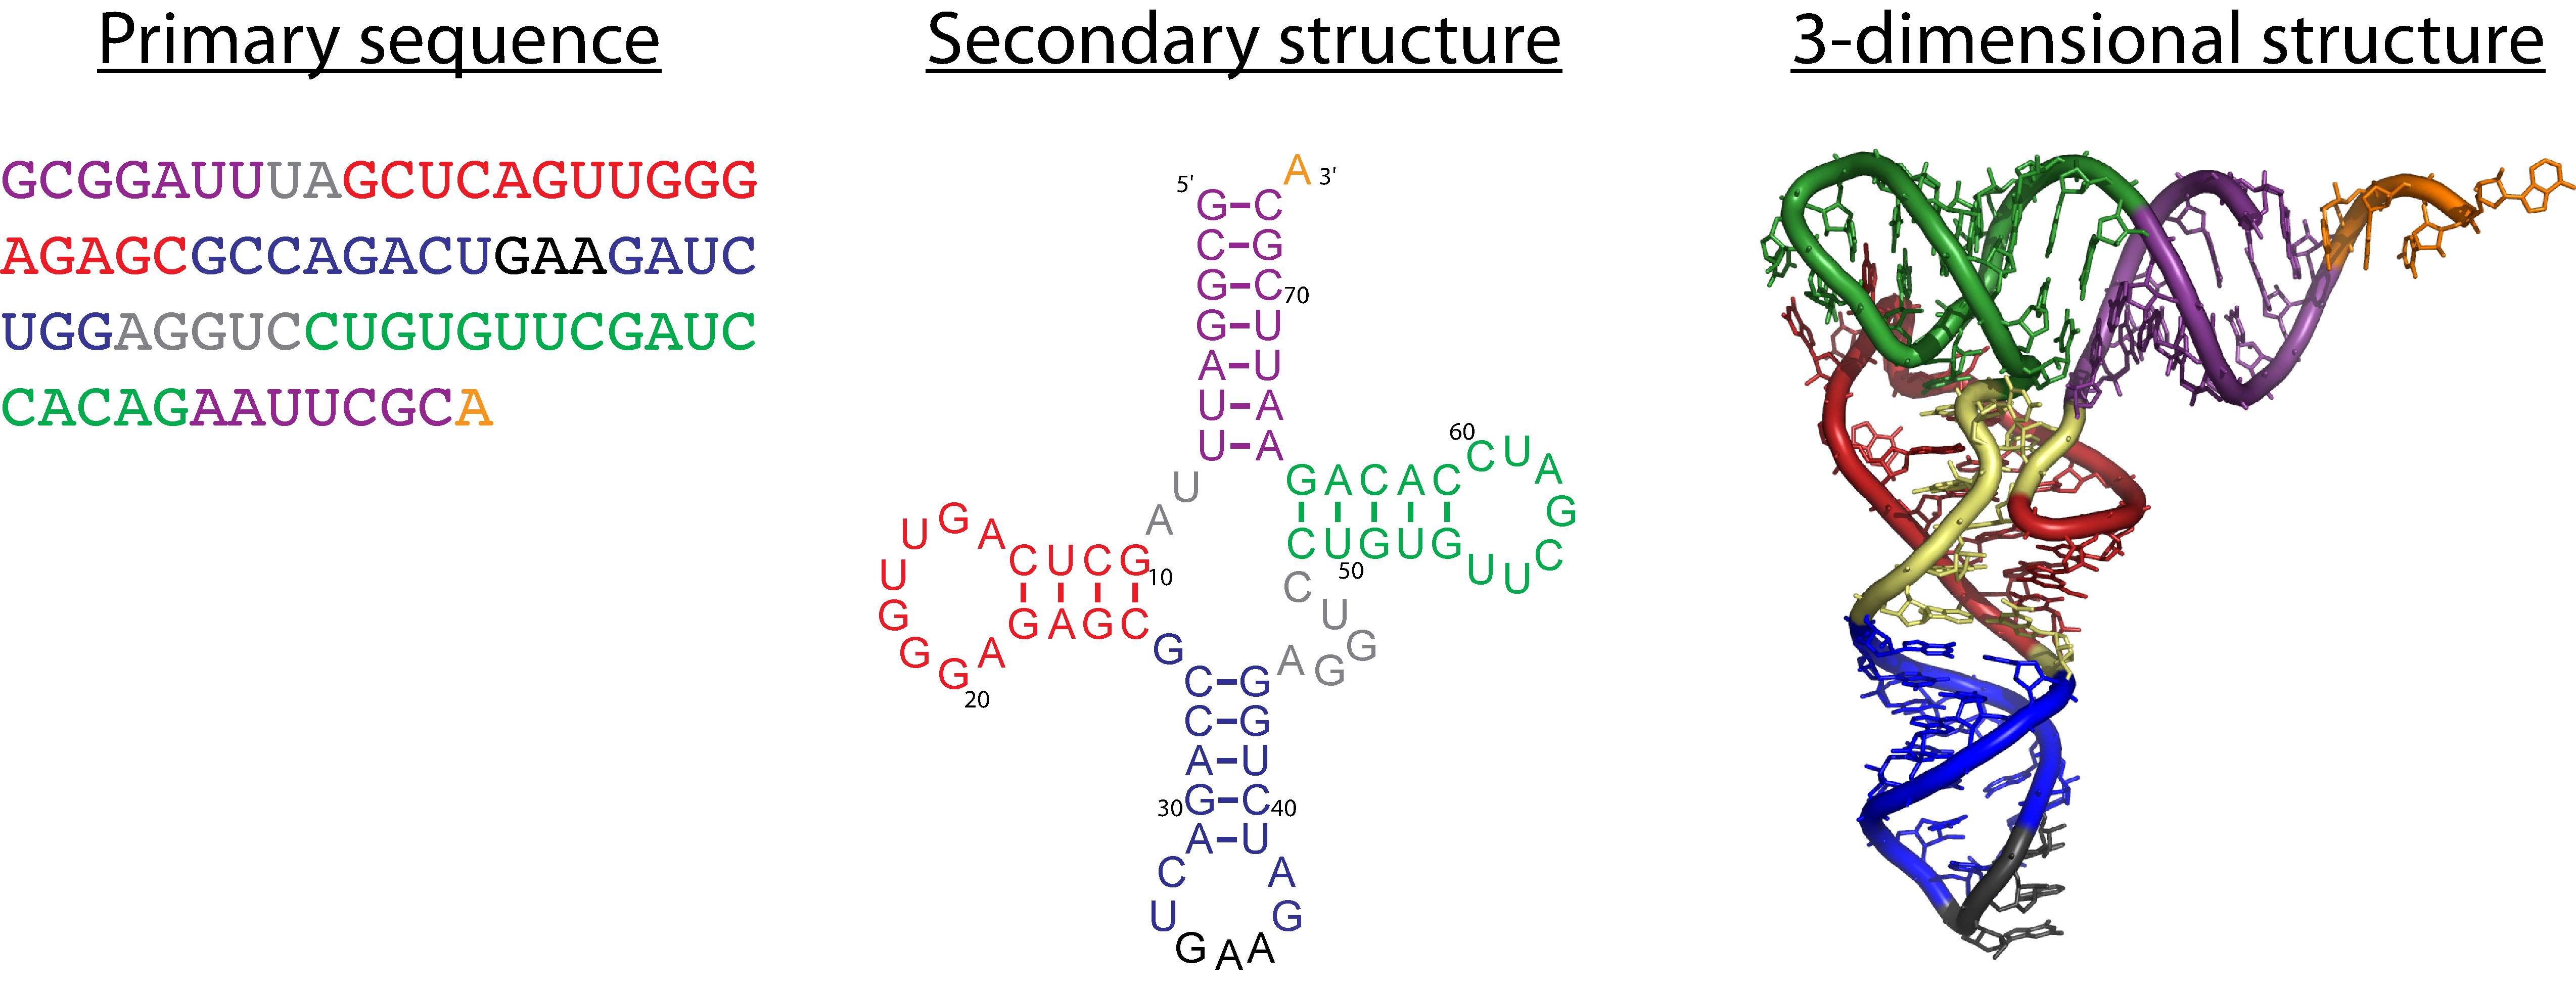
\includegraphics[width=10.5in]{figs/trna-123}
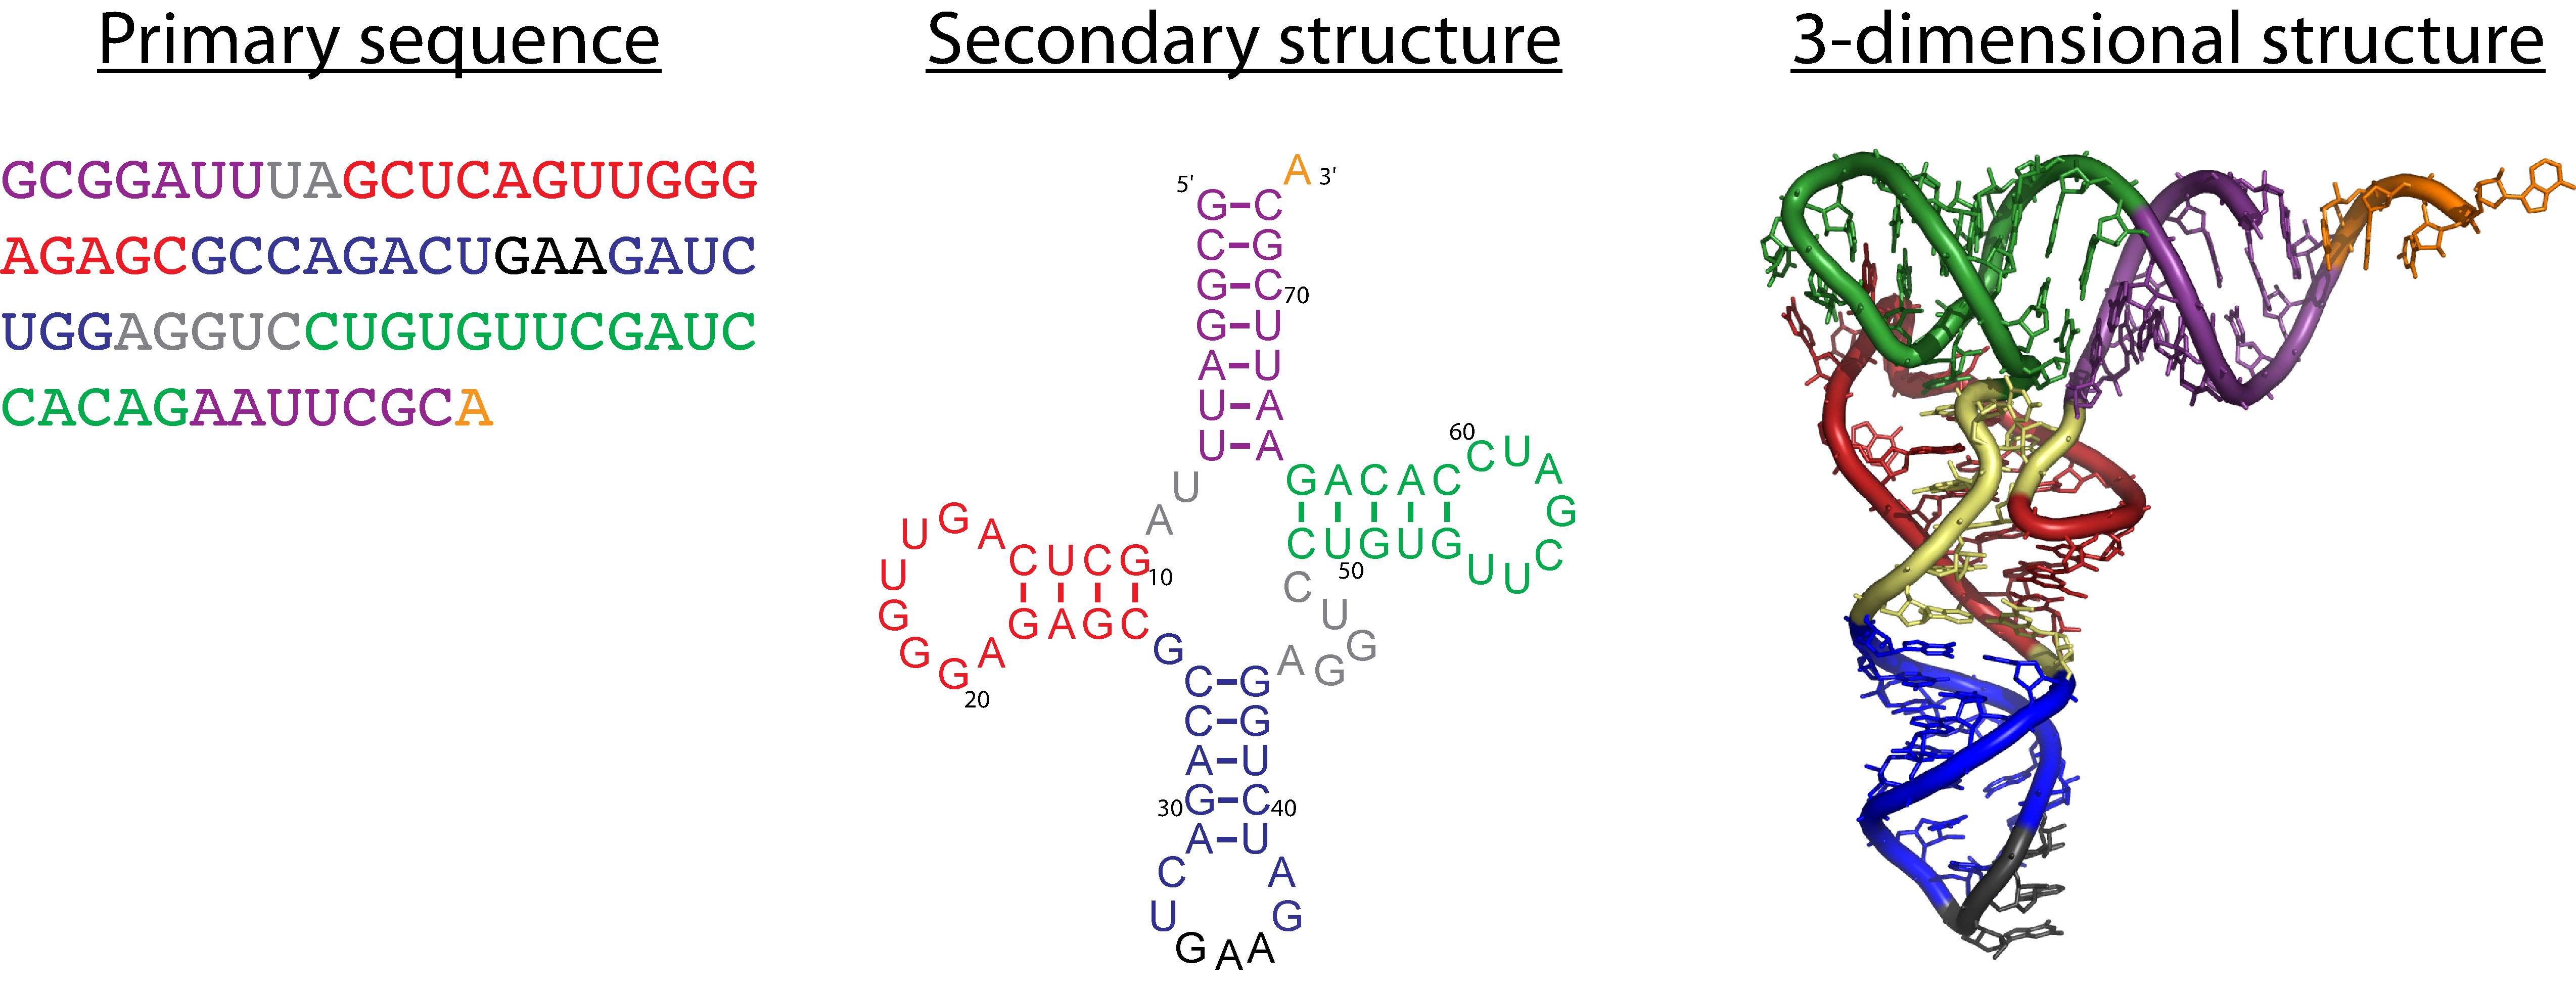
\includegraphics[width=9in]{figs/trna-123}

\end{center}

\vfill

\end{slide}
%%%%%%%%%%%%%%%%%%%%%%%%%%%%%%%%%%%%%%%%%%%%%%%%%%%%%%%%%%%%%%
\begin{slide}
\begin{center}
{\bf Many functional RNAs adopt a conserved 3-dimensional 
  structure}
\medskip

Three representations of a transfer RNA:

%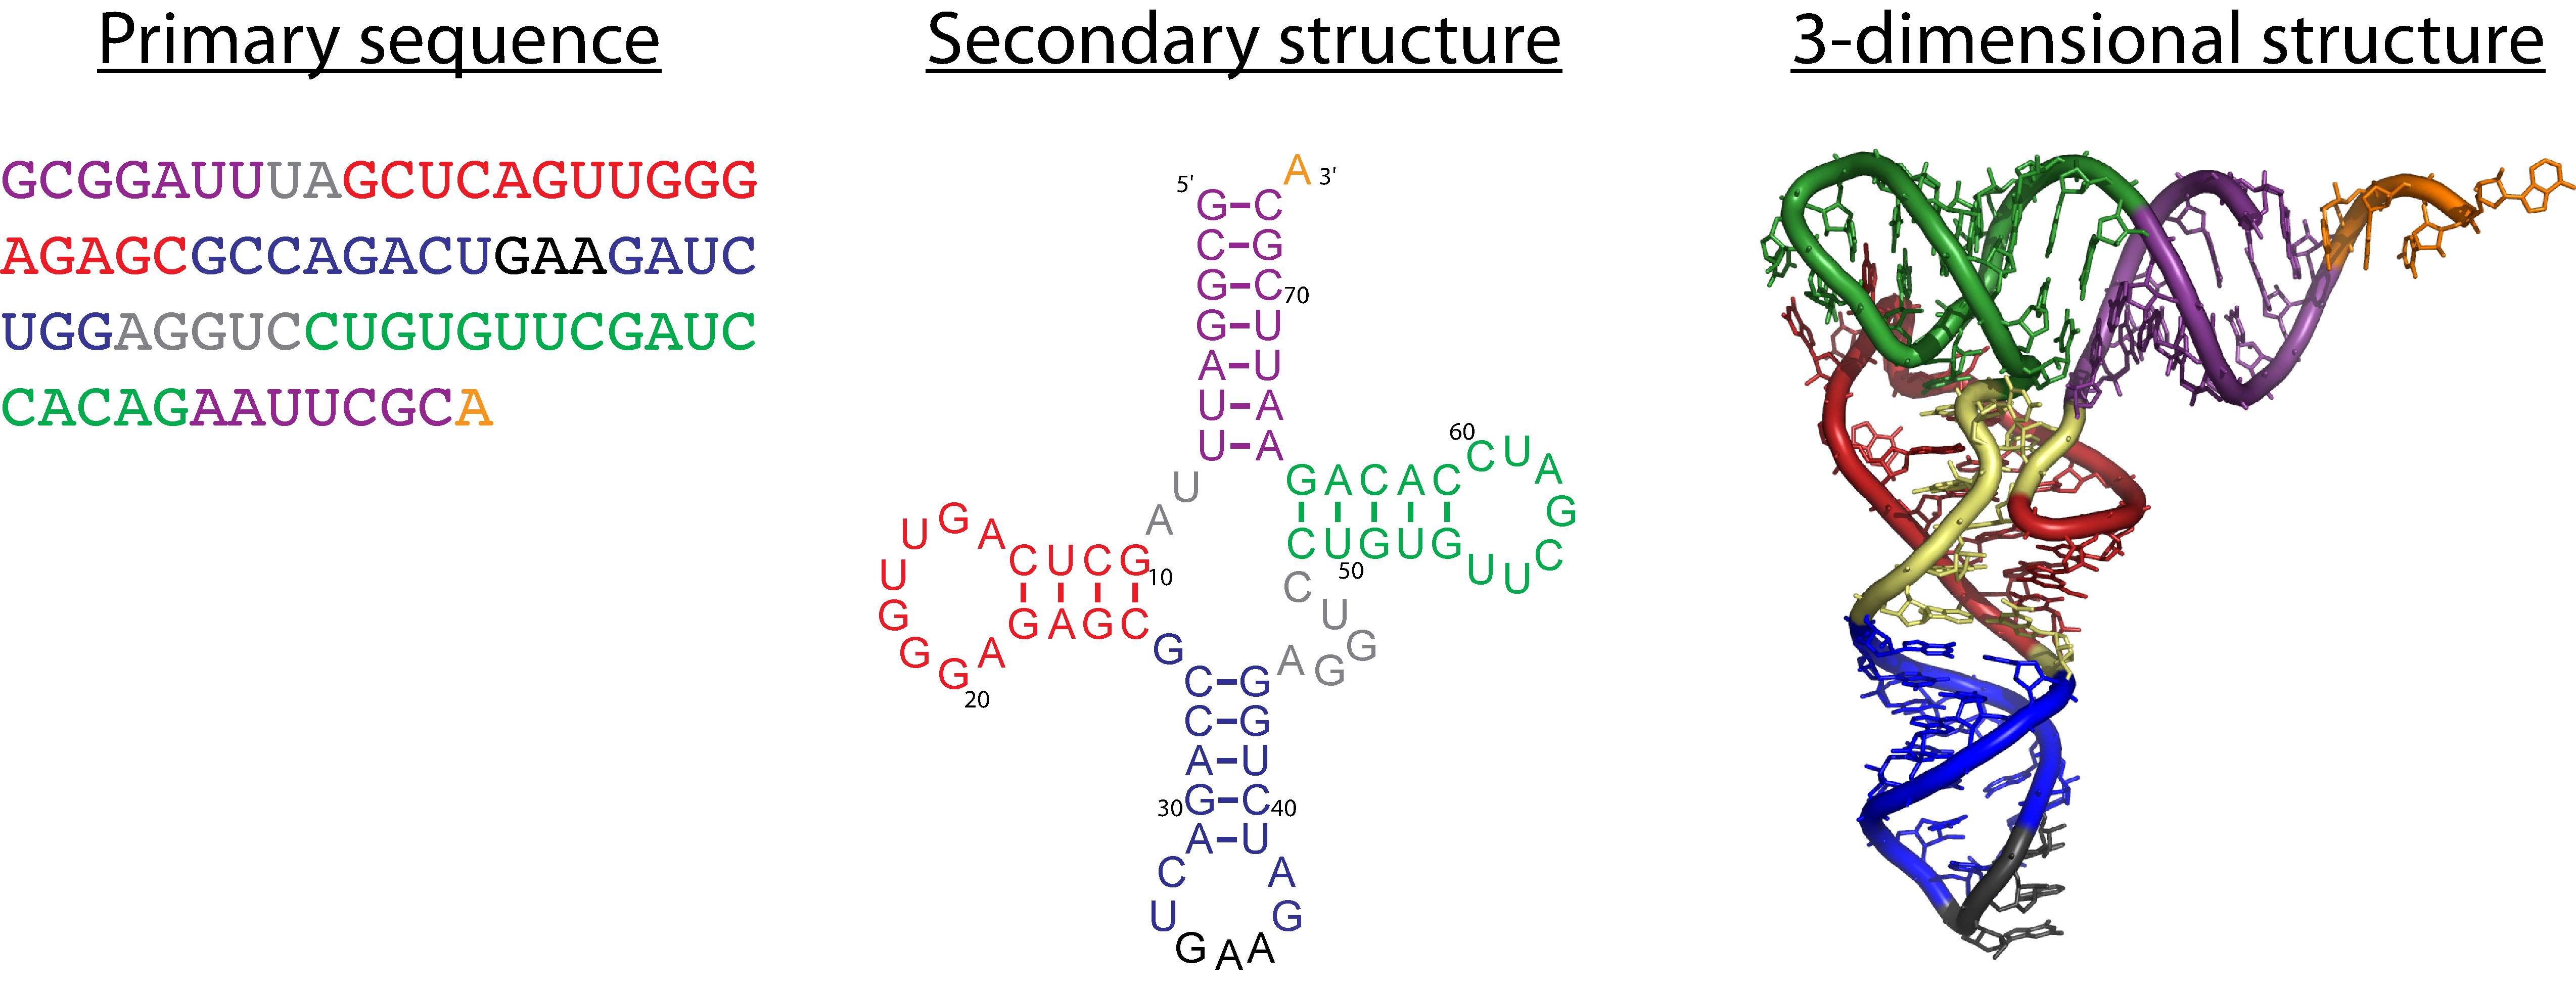
\includegraphics[width=10.5in]{figs/trna-123}
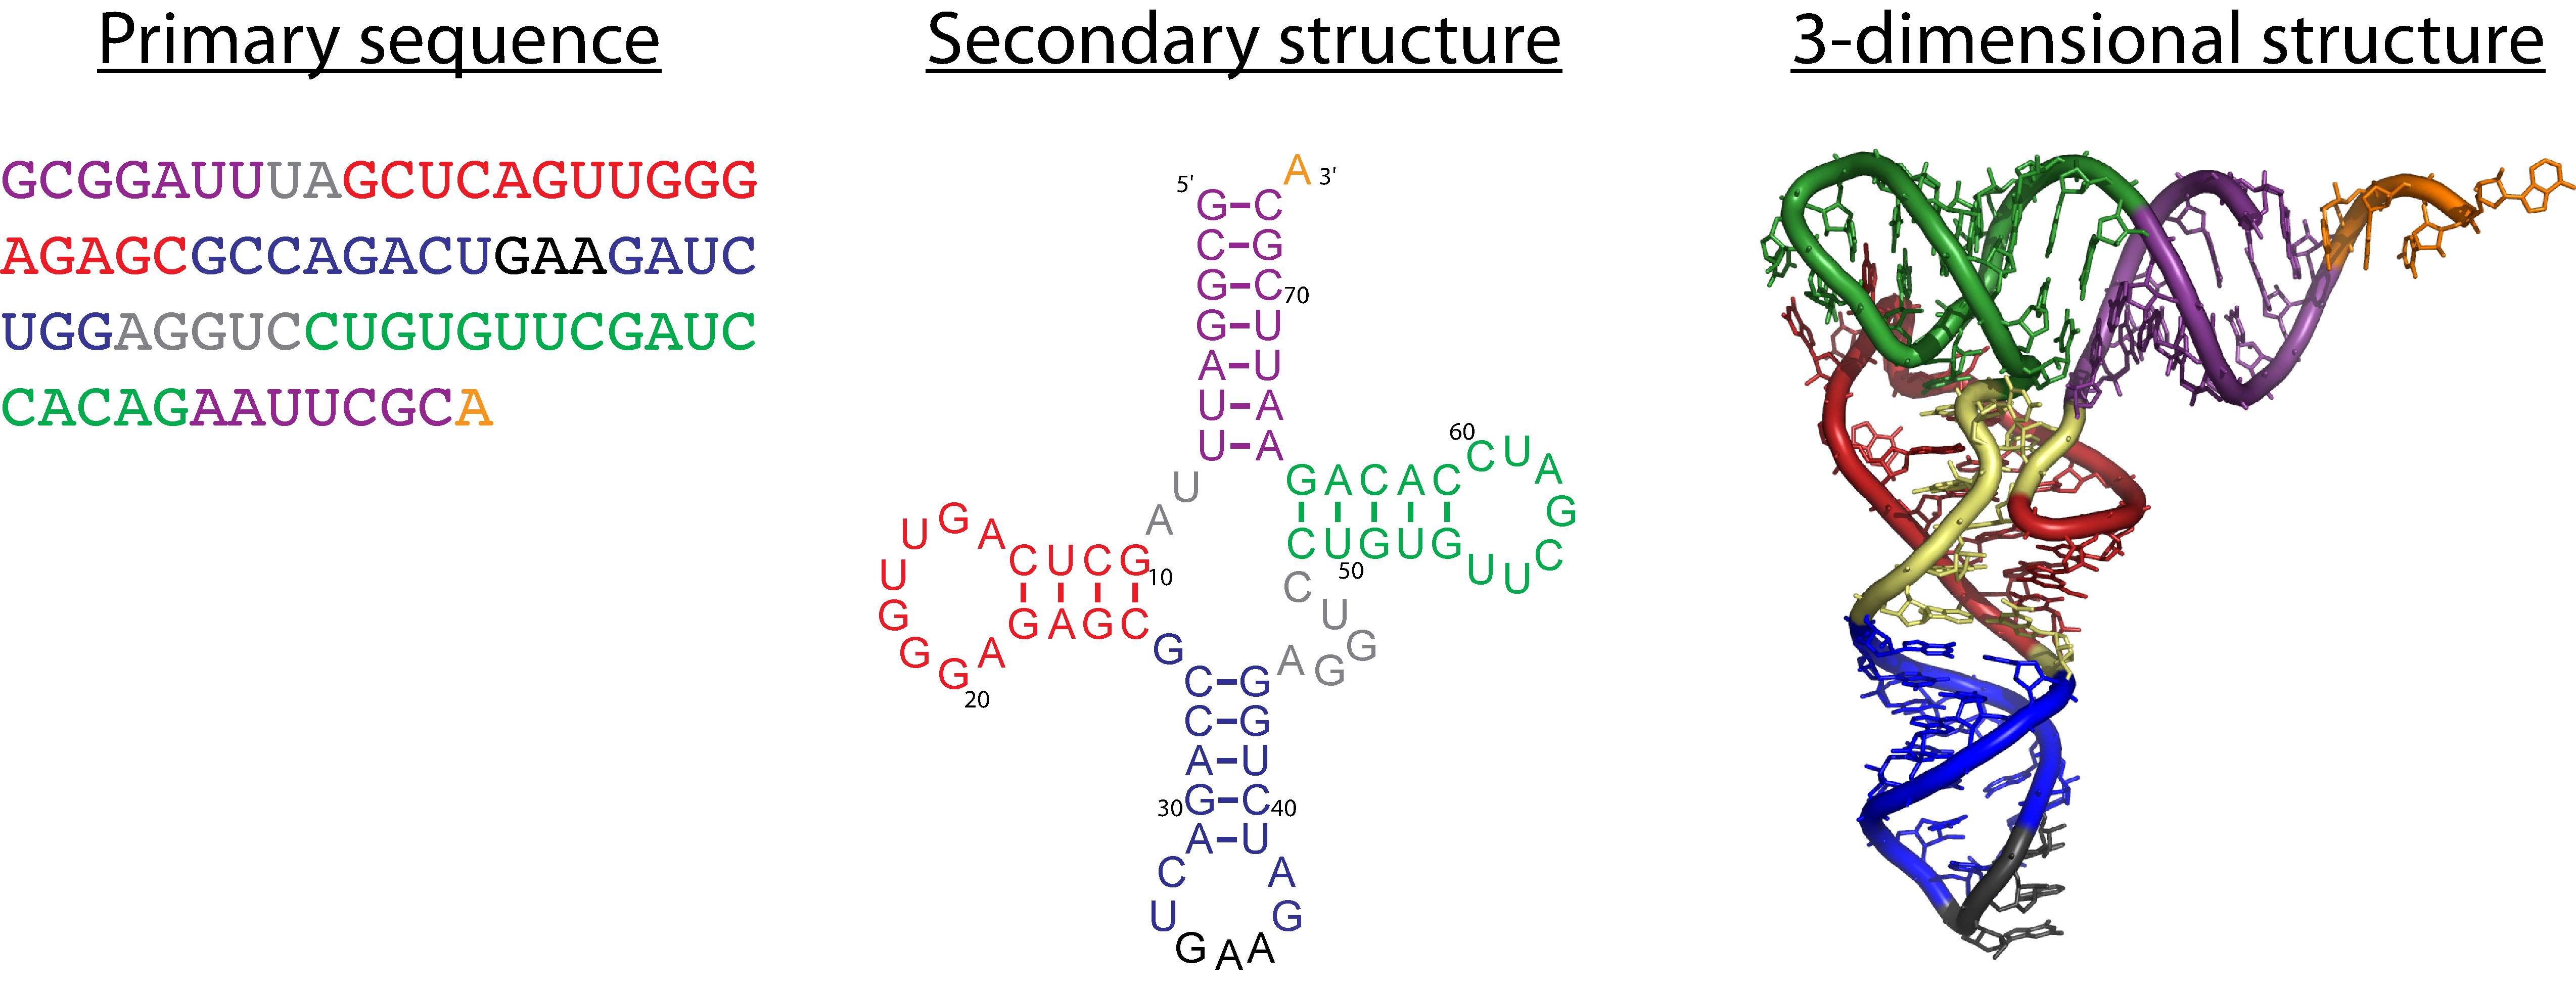
\includegraphics[width=9in]{figs/trna-123}
\end{center}

\begin{itemize}
\item
  BLAST: given a single sequence, search genomes for similar sequences.
\item
  BLAST cannot take advantage of:
\begin{itemize}
  \item sequence conservation, which varies across the gene
  \item secondary structure
\end{itemize}
\end{itemize}

\vfill

\end{slide}
%%%%%%%%%%%%%%%%%%%%%%%%%%%%%%%%%%%%%%%%%%%%%%%%%%%%%%%%%%%%%
\begin{slide}
\begin{center}
%\textbf{Comparative analysis of sequence families}: \\
\textbf{Sequence conservation provides \\ information for homology searches}

\medskip
Conservation levels vary across alignment columns.

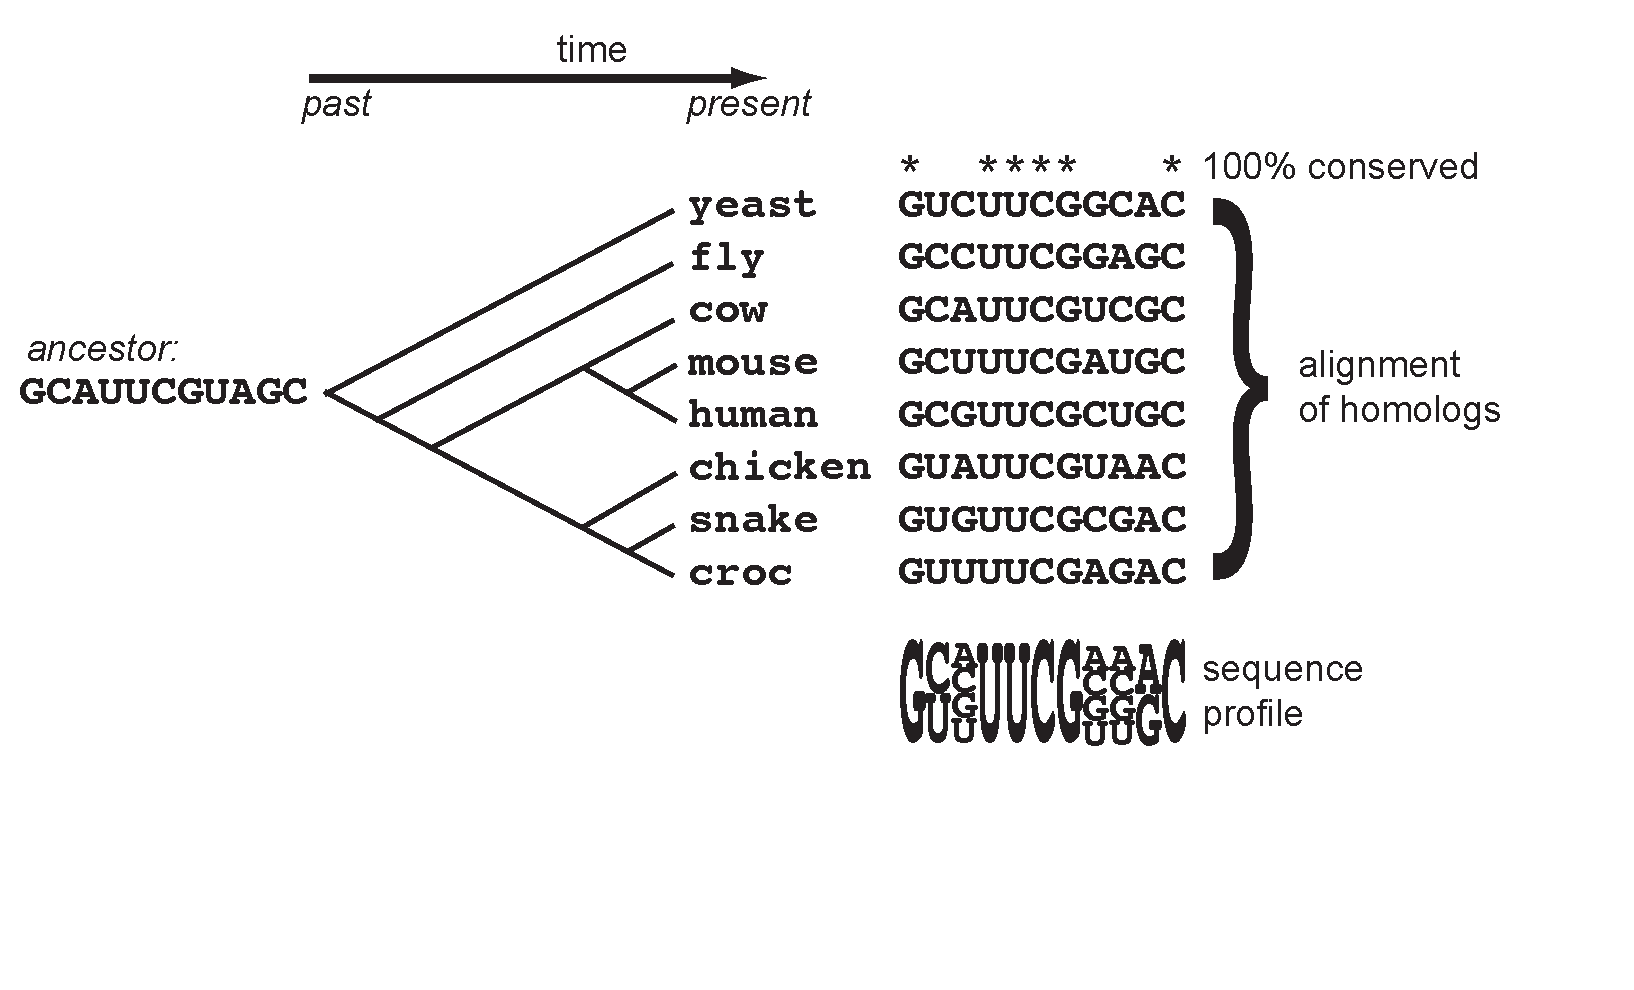
\includegraphics[width=10in]{figs/seqstructprofiles-seq1}
\end{center}

\vfill
\end{slide}
%%%%%%%%%%%%%%%%%%%%%%%%%%%%%%%%%%%%%%%%%%%%%%%%%%%%%%%%%%%%%%%%%%%%%%
\begin{slide}
\begin{center}
\textbf{Structure conservation provides additional information}
\medskip

Base-paired positions covary \\ to maintain Watson-Crick complementarity.

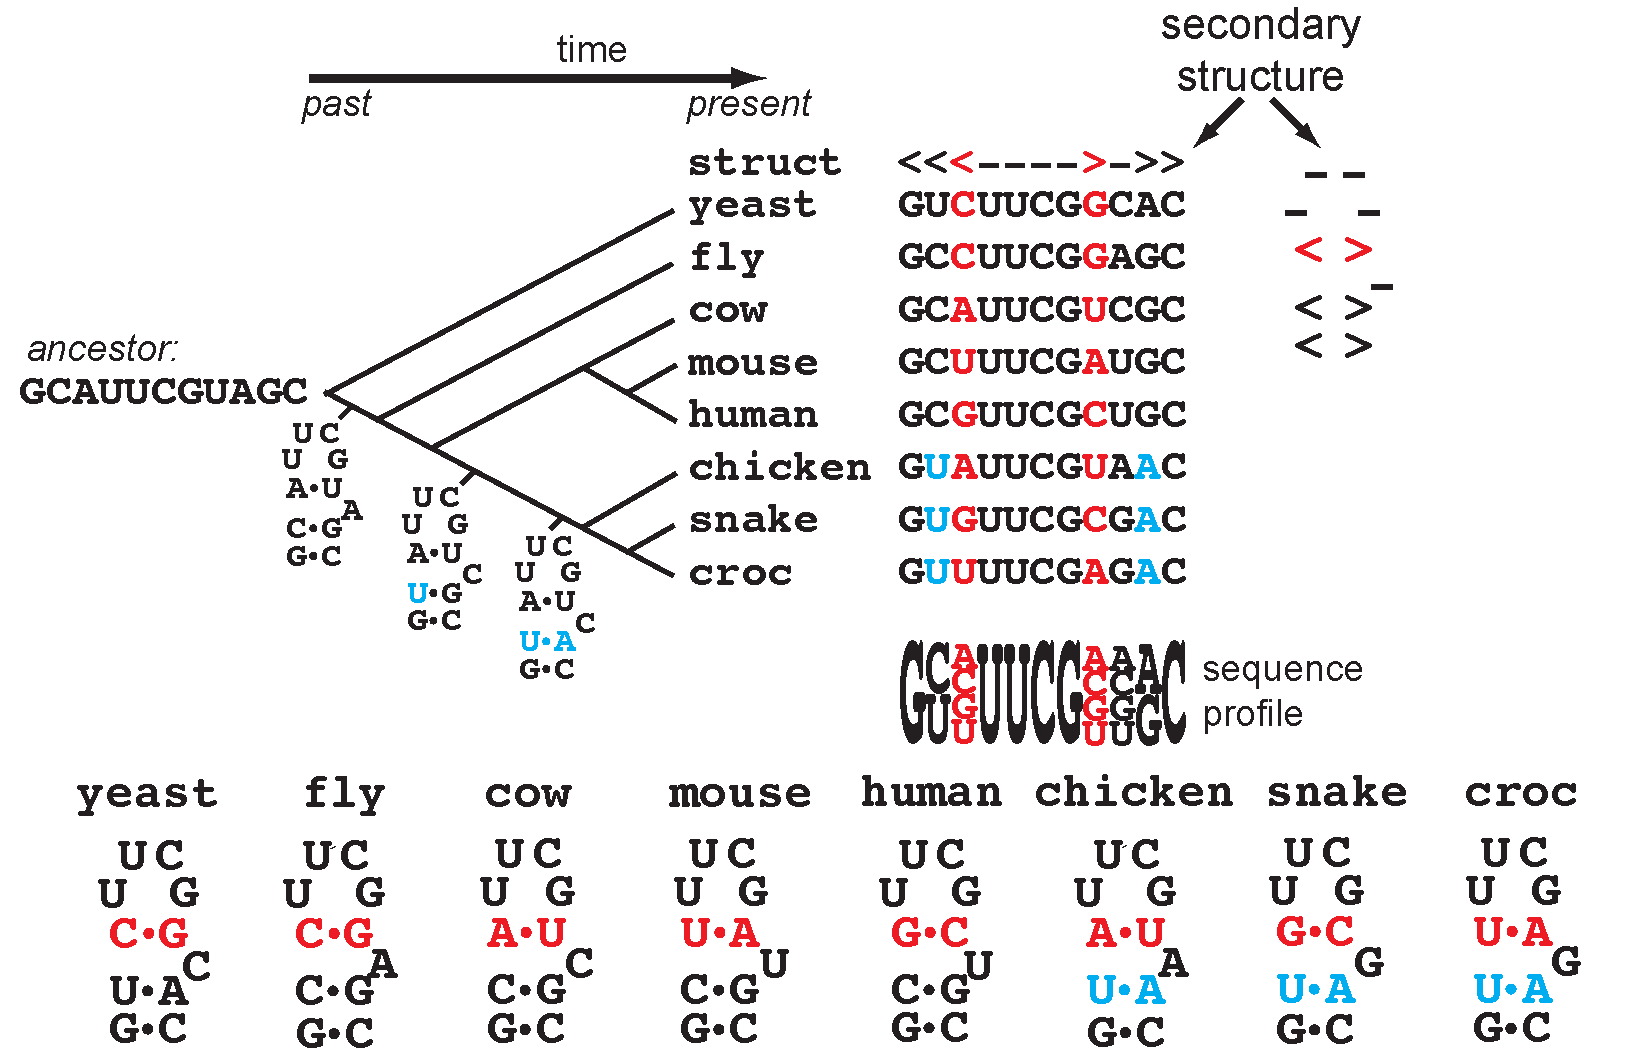
\includegraphics[width=10in]{figs/seqstructprofiles-struct2}
\end{center}

\vfill
\end{slide}
%%%%%%%%%%%%%%%%%%%%%%%%%%%%%%%%%%%%%%%%%%%%%%%%%%%%%%%%%%%%%%%%%%%%%%%%%%
\end{comment}
%%%%%%%%%%%%%%%%%%%%%%%%%%%%%%%%%%%%%%%%%%%%%%%%%%%%%%%%%%%%%%%%%%%%%%
\begin{slide}
\begin{center}
\textbf{Sequence conservation provides \\ information for homology searches}
\medskip

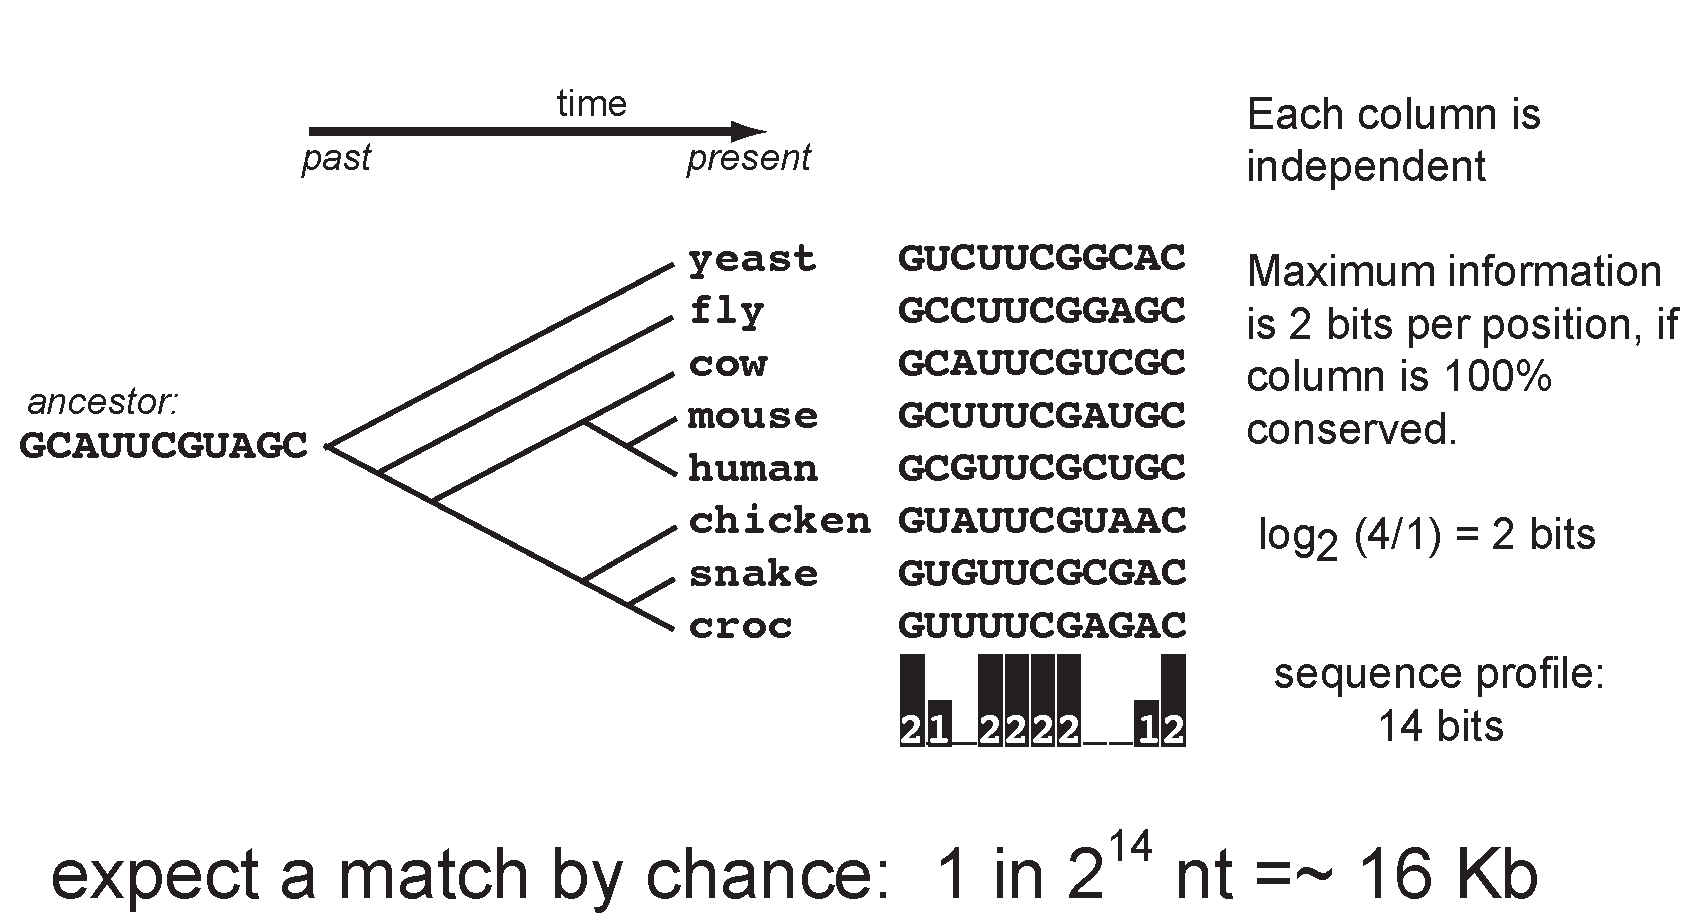
\includegraphics[width=9in]{figs/seqstructprofiles-2014-seqinfo}
\end{center}

\vfill
\end{slide}
%%%%%%%%%%%%%%%%%%%%%%%%%%%%%%%%%%%%%%%%%%%%%%%%%%%%%%%%%%%%%%%%%%%%%%%%%%
\begin{slide}
\begin{center}
\textbf{Structure contributes additional information from covariation}
\medskip

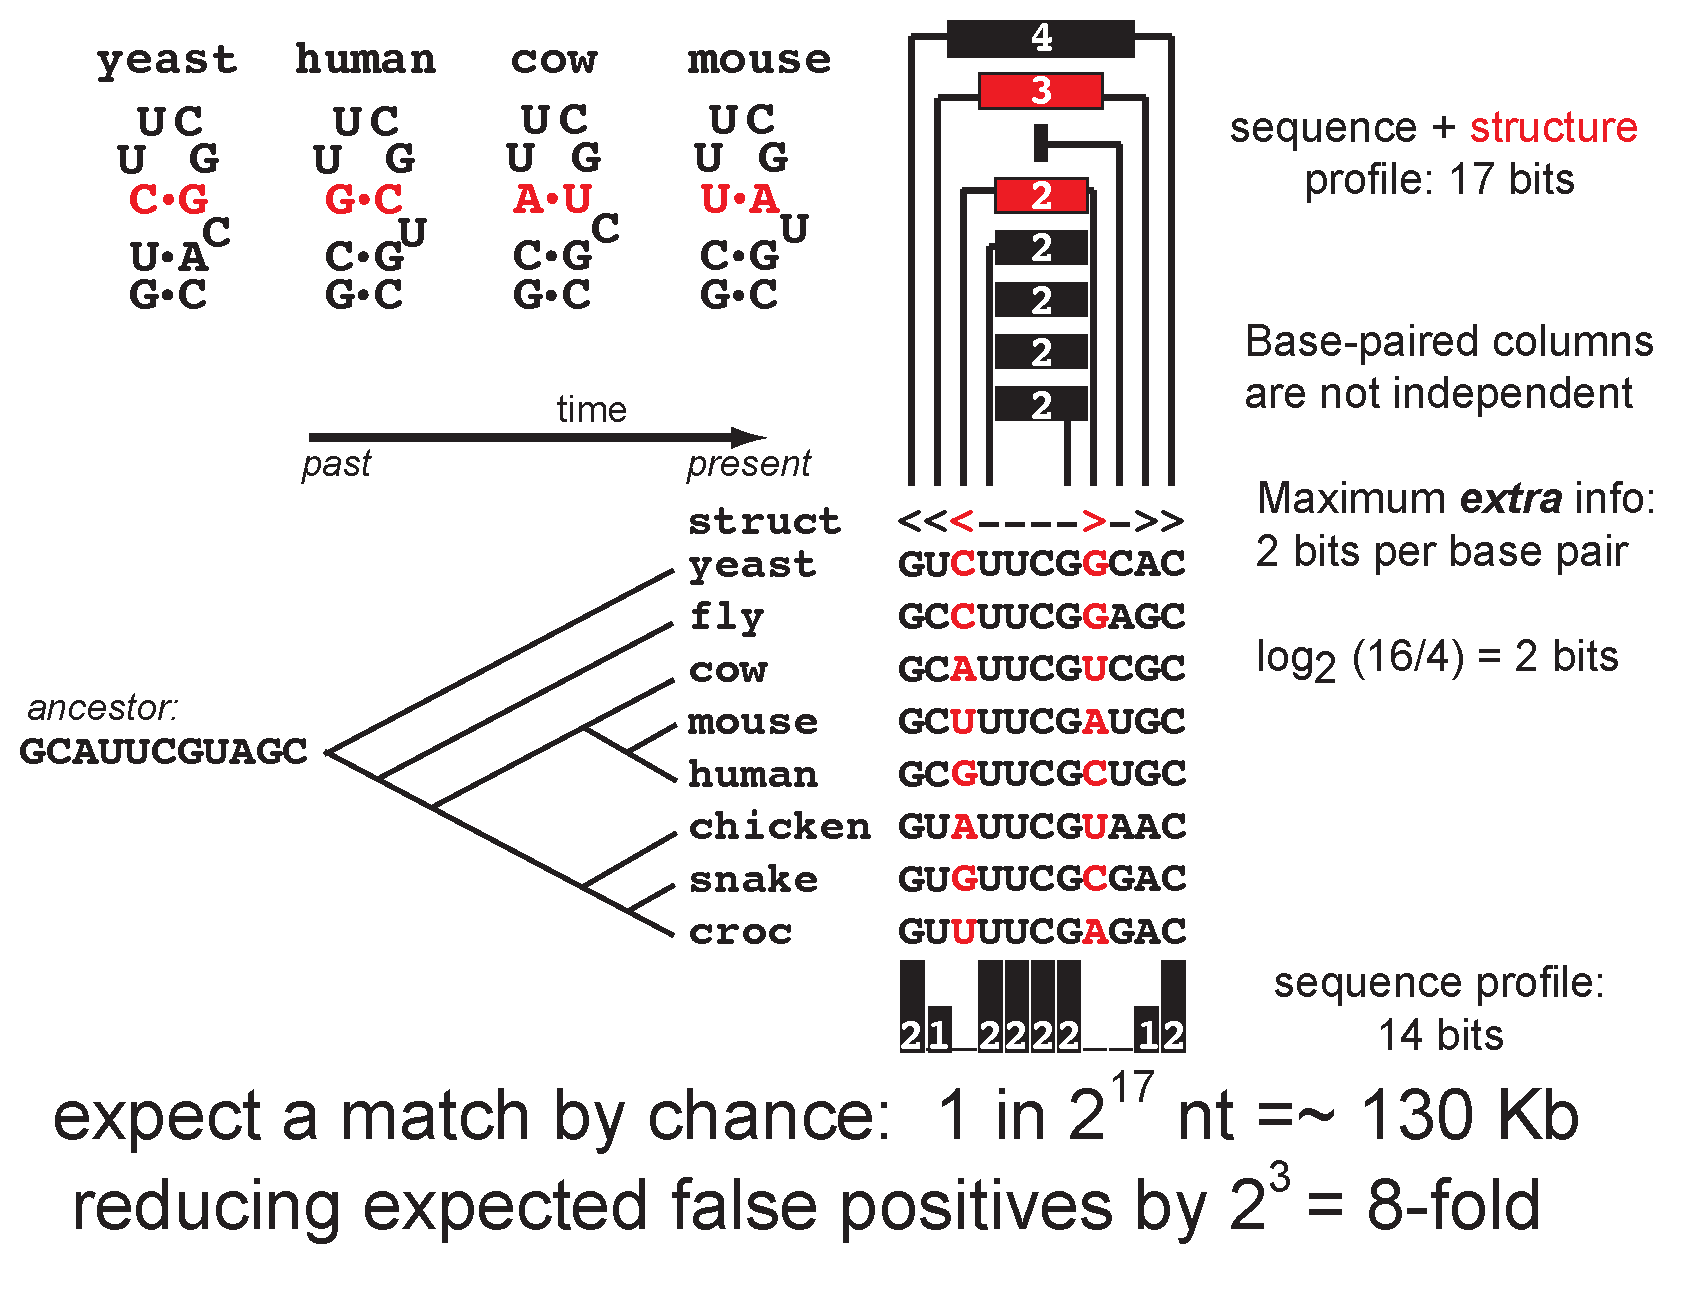
\includegraphics[width=9in]{figs/seqstructprofiles-2014-structinfo}
\end{center}

\vfill
\end{slide}
%%%%%%%%%%%%%%%%%%%%%%%%%%%%%%%%%%%%%%%%%%%%%%%%%%%%%%%%%%%%%%%%%%%%%%%%%%
\begin{slide}
\begin{center}
\textbf{Levels of sequence and structure conservation in RNA families}
\end{center}
\medskip

\begin{center}
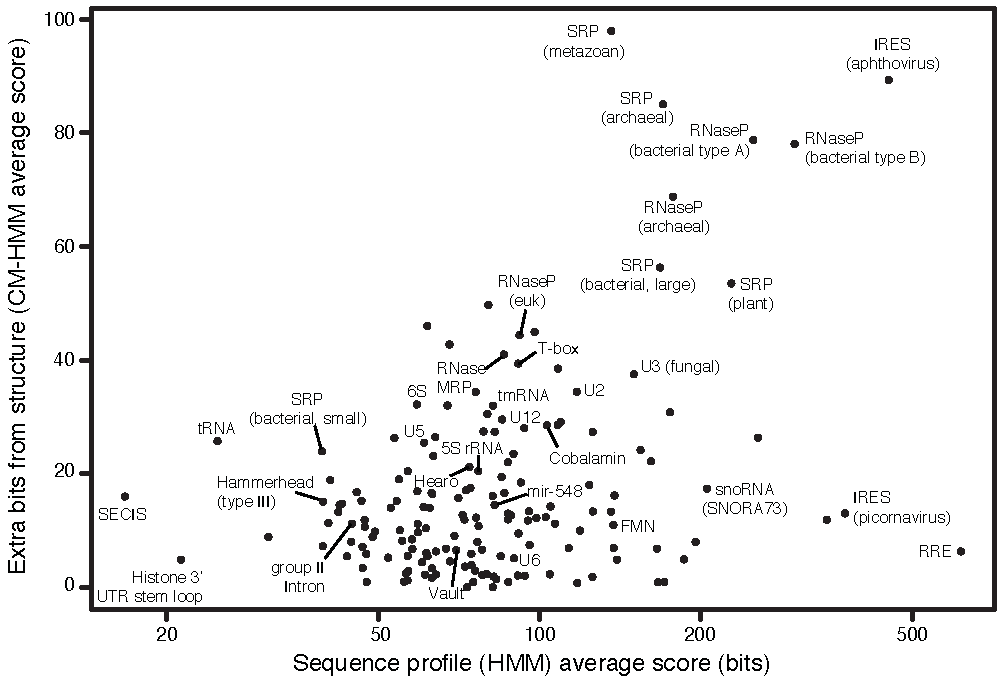
\includegraphics[height=6.5in]{figs/avgscores-rfam11}
\end{center}

\vfill

\end{slide}
%%%%%%%%%%%%%%%%%%%%%%%%%%%%%%%%%%%%%%%%%%%%%%%%%%%%%%%%%%%%%%%%%%%
\begin{slide}
\begin{center}
%\textbf{profile HMMs and covariance models}
\textbf{Eddy lab software for profile probabilistic models } (since 1994)
\end{center}
\medskip

\begin{center}
\small
\begin{tabular}{r|cc} 
%             &         & sequence \\
%             & sequence& and structure \\
%             & profiles& profiles \\ \hline
             & sequence & sequence and \\
             & profiles & structure profiles \\ \hline
  \\
  models     & profile HMMs     & {\color{red} covariance models (CMs)} \\ 
  \\
  software   & {\sc HMMER}      & {\sc Infernal} \\ 
  \\
  main use   & proteins,         & structural RNAs \\ 
             & repetitive DNA elements &  \\
  \\
  databases  & {\sc Pfam} and \sc{Dfam}       & {\sc Rfam} \\
             & (16712 and 4150 entries) & (2791 families) \\
  \\
%  primary sequence & yes & yes \\
%  \\
%  secondary structure & no & yes \\
%  \\
%  algorithms & Viterbi, Forward & CYK, Inside \\
%%             & Forward & Inside \\
%             &         & \\
%  complexity & $O(LN)$ & $O(LN^{2} log N)$ \\
%  \\
  performance& faster but    & slower but    \\
  for RNAs   & less accurate & more accurate \\
\end{tabular}

%\hspace{1.2in}
\includegraphics[height=2in]{figs/hmmer_logo}\hspace{1.05in}\includegraphics[height=2.6in]{figs/infernal_logo}
\hspace{1.8in}
\includegraphics[height=2.7in]{figs/hmmer-infernal-refs-2018}

\end{center}

\vfill

\end{slide}
%%%%%%%%%%%%%%%%%%%%%%%%%%%%%%%%%%%%%%%%%%%%%%%%%%%%%%%%%%%%%%%
%%%%%%%%%%%%%%%%%%%%%%%%%%%%%%%%%%%%%%%%%%%%%%%%%%%%%%%%%%%%%%%
%%%%%%%%%%%%%%%%%%%%%%%%%%%%%%%%%%%%%%%%%%%%%%%%%%%%%%%%%%%%%%%
%%%%%%%%%%%%%%%%%%%%%%%%%%%%%%%%%%%%%%%%%%%%%%%%%%%%%%%%%%%%%%%
%%%%%%%%%%%%%%%%%%%%%%%%%%%%%%%%%%%%%%%%%%%%%%%%%%%%%%%%%%%%%%%
%%%%%%%%%%%%%%%%%%%%%%%%%%%%%%%%%%%%%%%%%%%%%%%%%%%%%%%%%%%%%%%
%%%%%%%%%%%%%%%%%%%%%%%%%%%%%%%%%%%%%%%%%%%%%%%%%%%%%%%%%%%%%%%%%%%%%
\begin{slide}
\begin{center}
%\textbf{profile HMMs and covariance models}
\textbf{Profile HMMs: sequence family models built from alignments}
\end{center}

\center{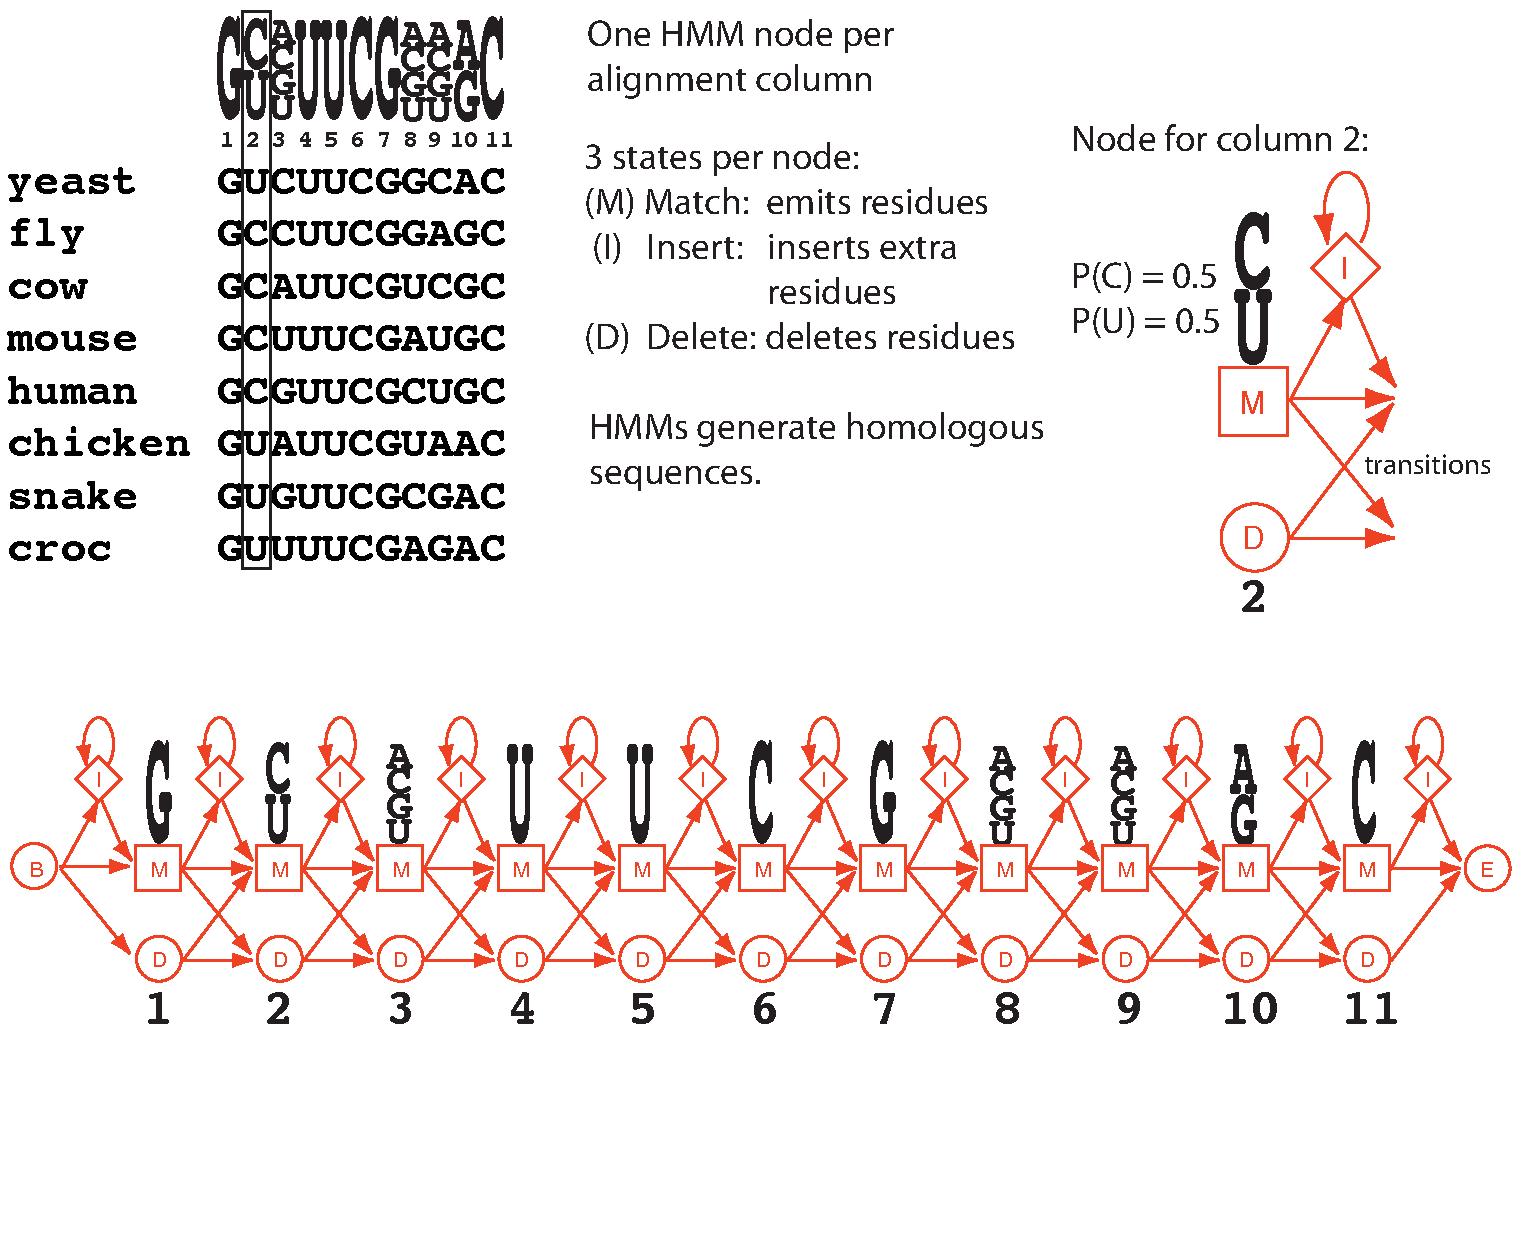
\includegraphics[height=6.625in]{figs/hmm}}

%An HMM generates ``homologous'' sequences.

\end{slide}
%%%%%%%%%%%%%%%%%%%%%%%%%%%%%%%%%%%%%%%%%%%%%%%%%%%%%%%%%%%%%%%
\begin{slide}
\begin{center}
%\textbf{profile HMMs and covariance models}
\textbf{Profile HMMs: sequence family models built from alignments}
\end{center}

\center{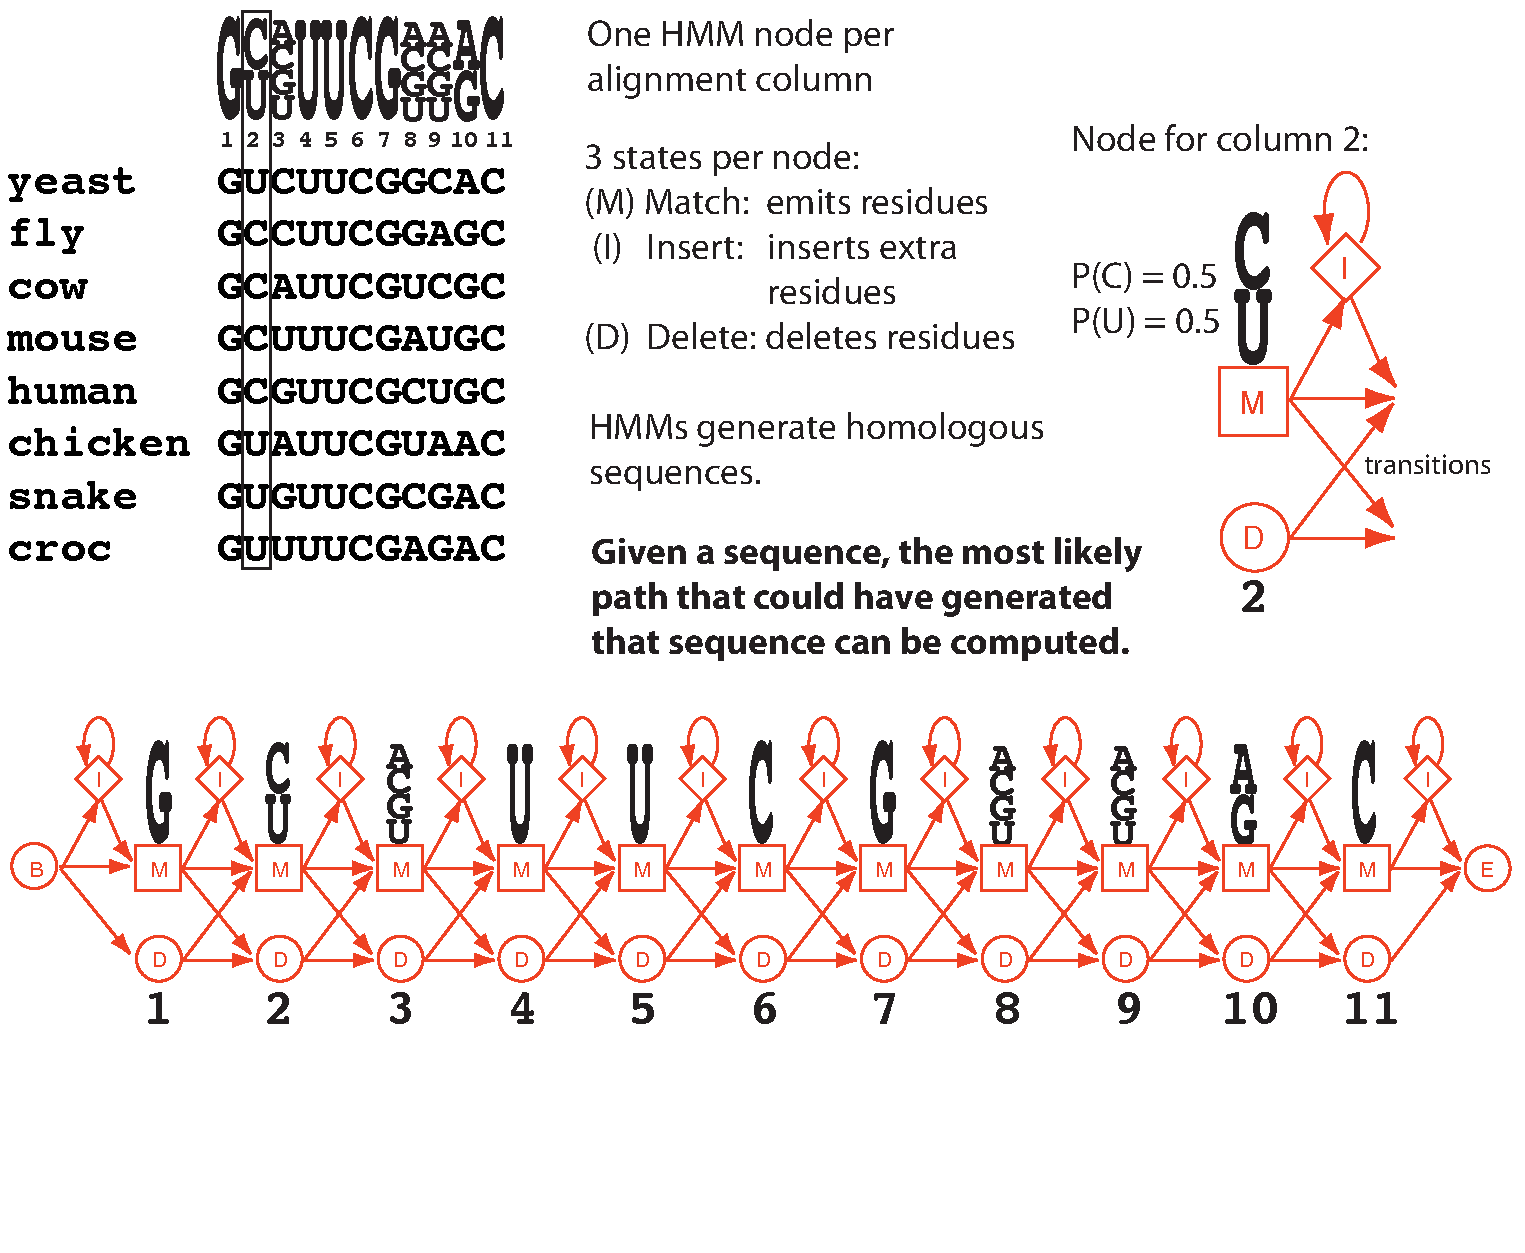
\includegraphics[height=6.625in]{figs/hmm-given}}
\end{slide}
%%%%%%%%%%%%%%%%%%%%%%%%%%%%%%%%%%%%%%%%%%%%%%%%%%%%%%%%%%%%%%%
\begin{slide}
\begin{center}
%\textbf{profile HMMs and covariance models}
\textbf{Profile HMMs: sequence family models built from alignments}
\end{center}

\center{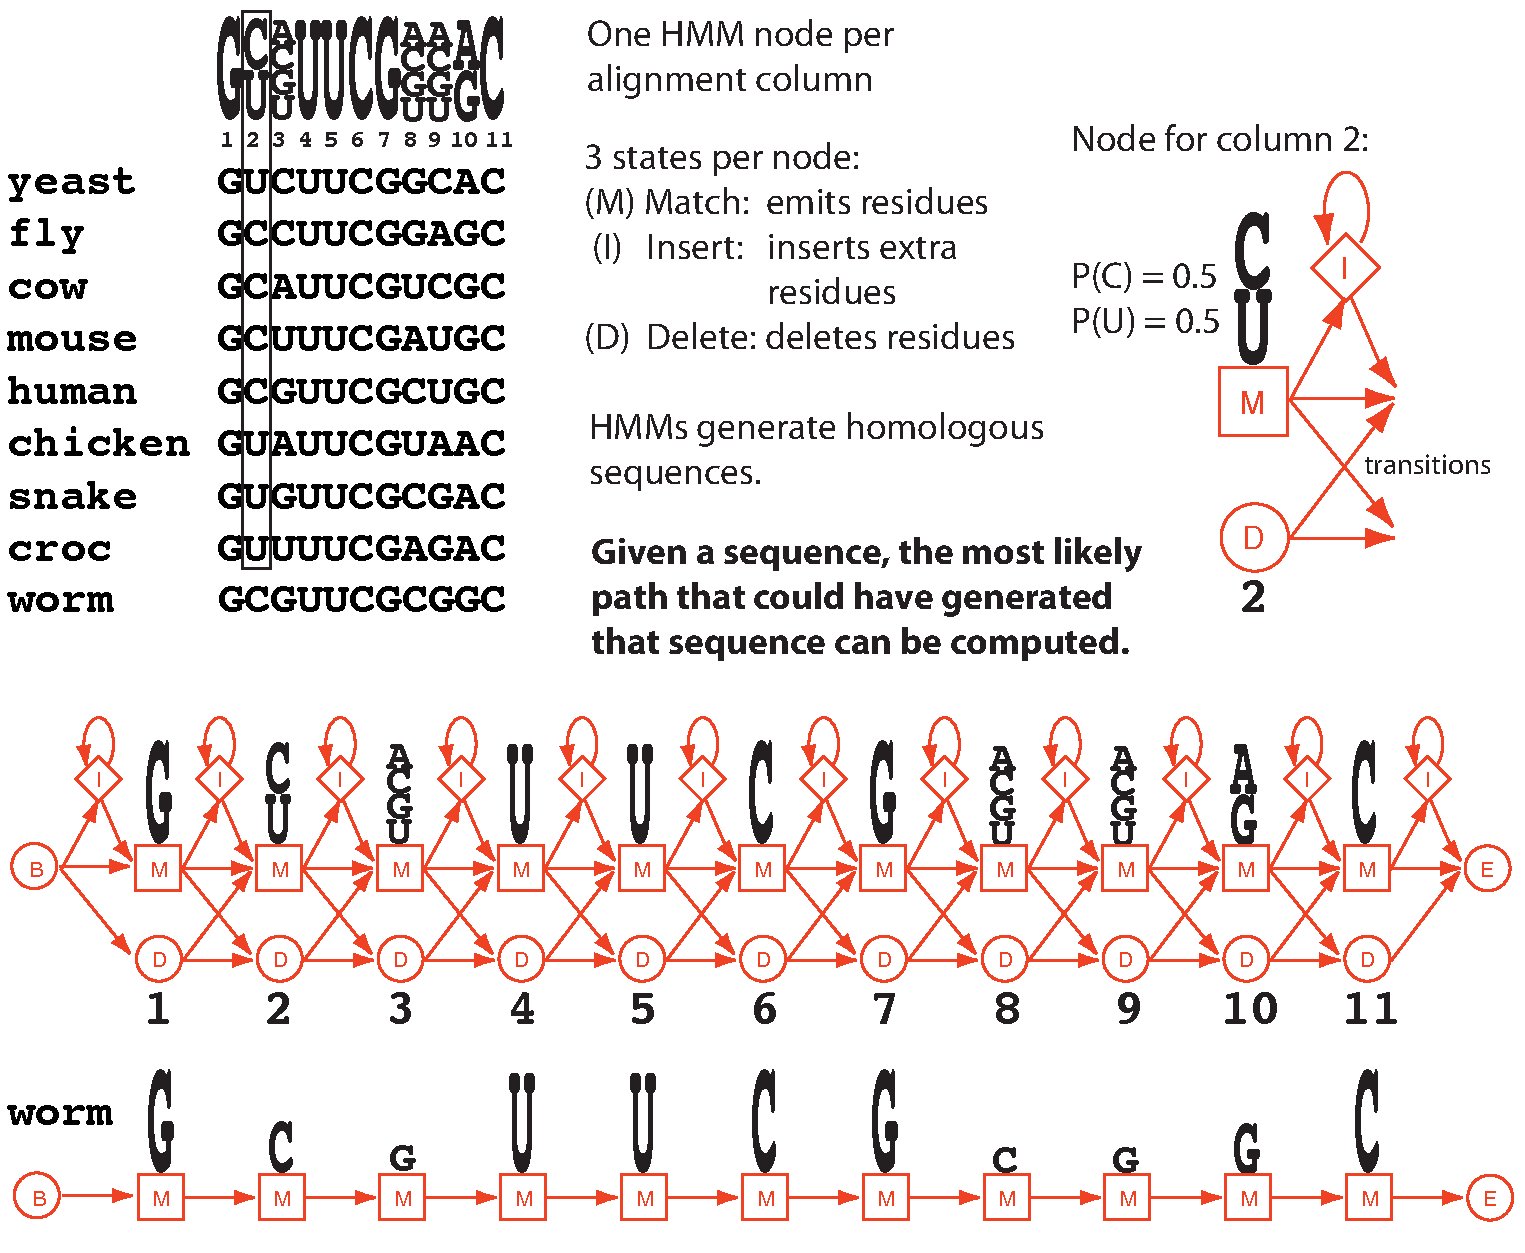
\includegraphics[height=6.625in]{figs/hmm-worm}}
\end{slide}
%%%%%%%%%%%%%%%%%%%%%%%%%%%%%%%%%%%%%%%%%%%%%%%%%%%%%%%%%%%
\begin{slide}
\begin{center}
%\textbf{profile HMMs and covariance models}
\textbf{Profile HMMs: sequence family models built from alignments}
\end{center}

\center{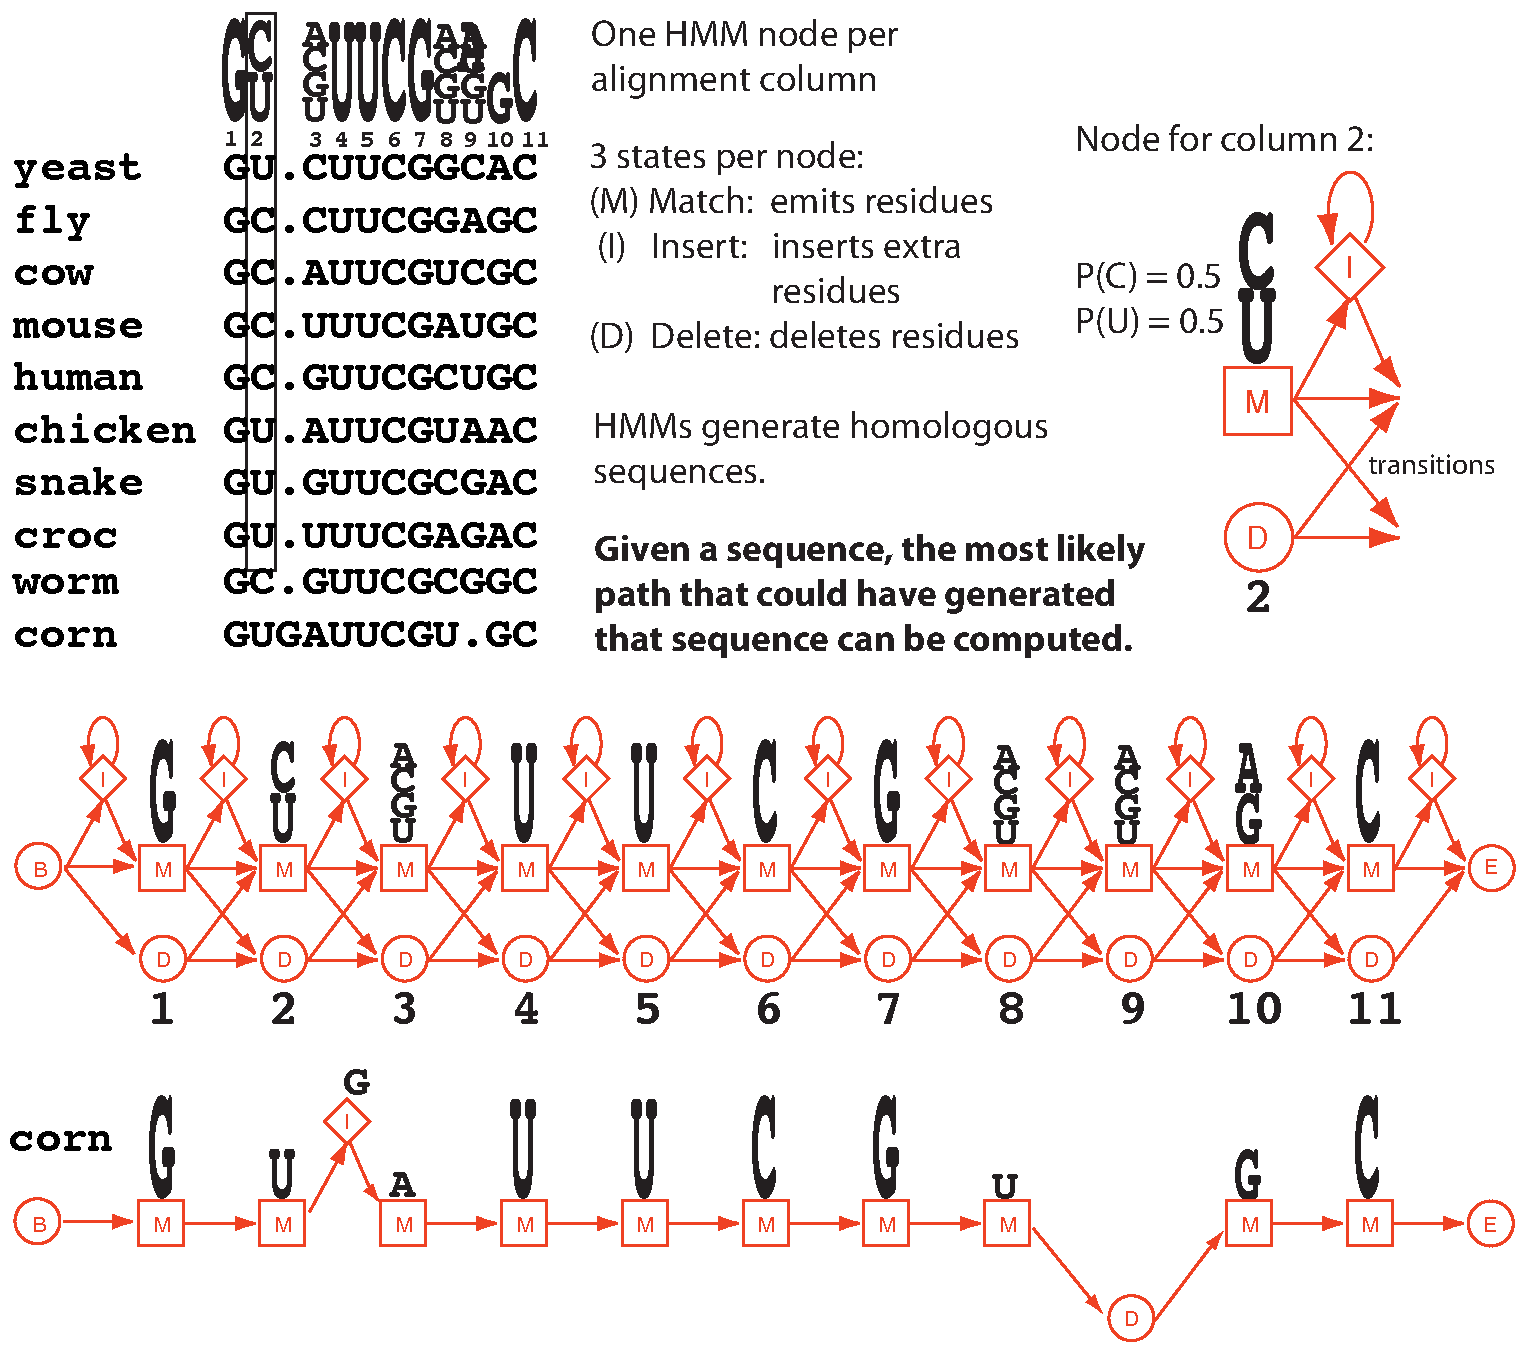
\includegraphics[height=6.625in]{figs/hmm-corn}}
\end{slide}
%%%%%%%%%%%%%%%%%%%%%%%%%%%%%%%%%%%%%%%%%%%%%%%%%%%%%%%%%%%%%%%
\begin{slide}
\begin{center}
%\textbf{profile HMMs and covariance models}
\textbf{Covariance models (CMs) are built \\ from structure-annotated alignments}
\end{center}

\center{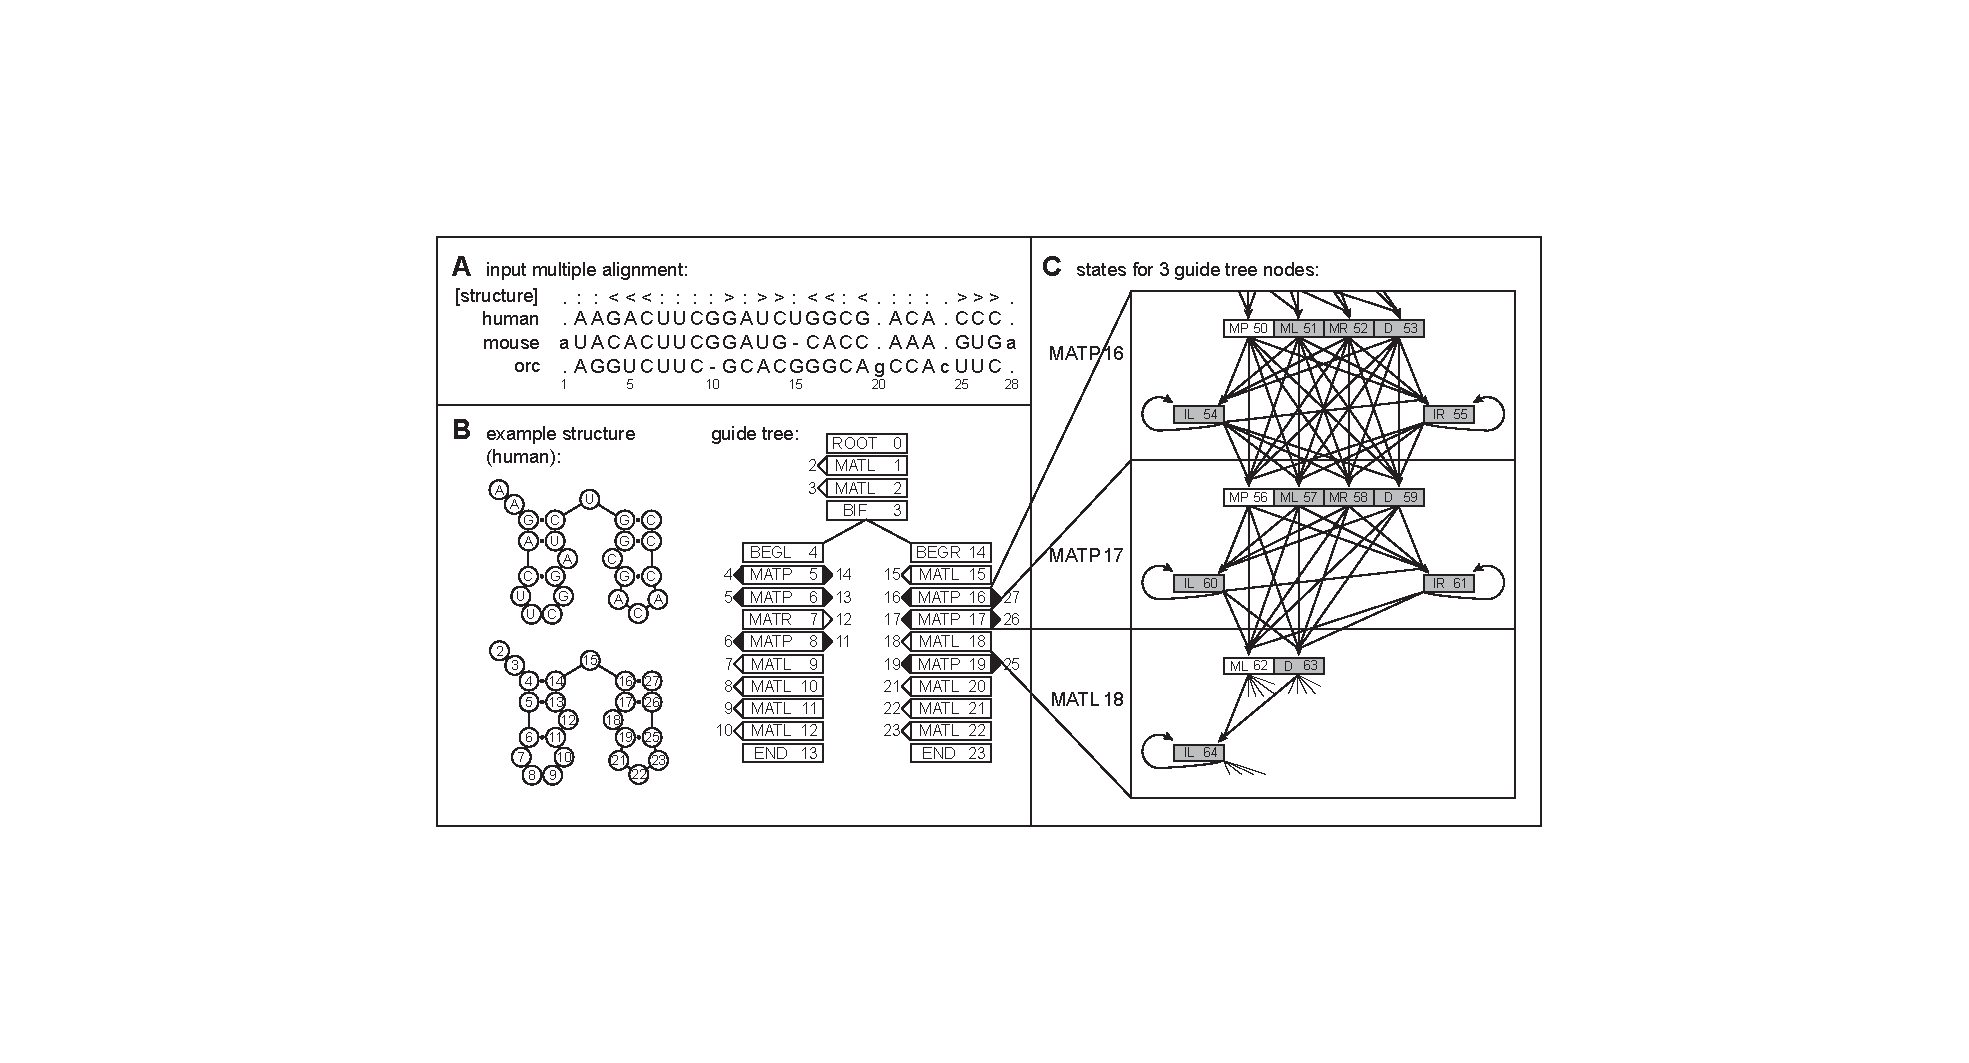
\includegraphics[width=7in]{figs/cmintro_bandcyk}}

\center{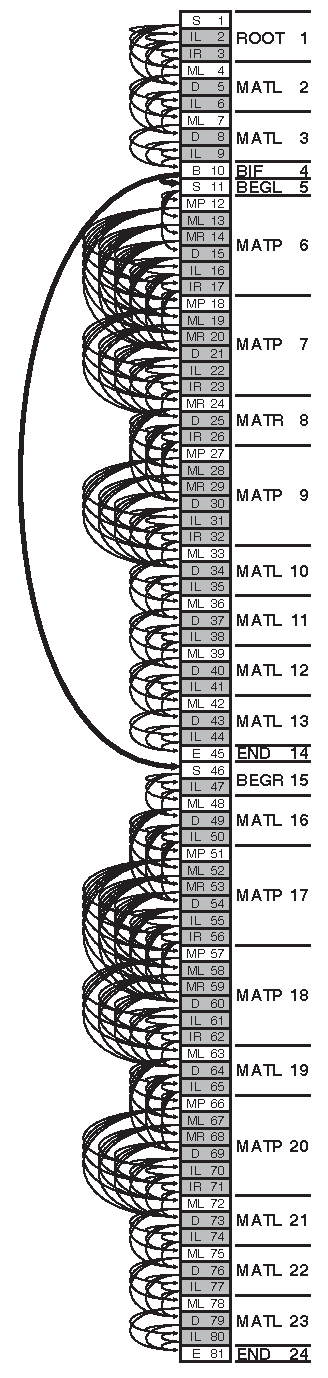
\includegraphics[width=2in,angle=270]{figs/cm-graph-small}}

\vfill

\end{slide}
%%%%%%%%%%%%%%%%%%%%%%%%%%%%%%%%%%%%%%%%%%%%%%%%%%%%%%%%%%%%%%%%%%

%%%%%%%%%%%%%%%%%%%%%%%%%%%%%%%%%%%%%%%%%%%%%%%%%%%%%%%%%%%%%%%
%%%%%%%%%%%%%%%%%%%%%%%%%%%%%%%%%%%%%%%%%%%%%%%%%%%%%%%%%%%%%%%
%%%%%%%%%%%%%%%%%%%%%%%%%%%%%%%%%%%%%%%%%%%%%%%%%%%%%%%%%%%%%%%
%%%%%%%%%%%%%%%%%%%%%%%%%%%%%%%%%%%%%%%%%%%%%%%%%%%%%%%%%%%%%%%
%%%%%%%%%%%%%%%%%%%%%%%%%%%%%%%%%%%%%%%%%%%%%%%%%%%%%%%%%%%%%%%
%%%%%%%%%%%%%%%%%%%%%%%%%%%%%%%%%%%%%%%%%%%%%%%%%%%%%%%%%%%%%%%
\begin{slide}
\begin{center}

\textbf{Infernal outperforms primary-sequence based methods on our
  benchmark (and others\footnote{Freyhult EK, Bollback JP, Gardner
    PP. Genome Res. 2007 17: 117-125.}, not shown)}

\end{center}
\medskip

\center{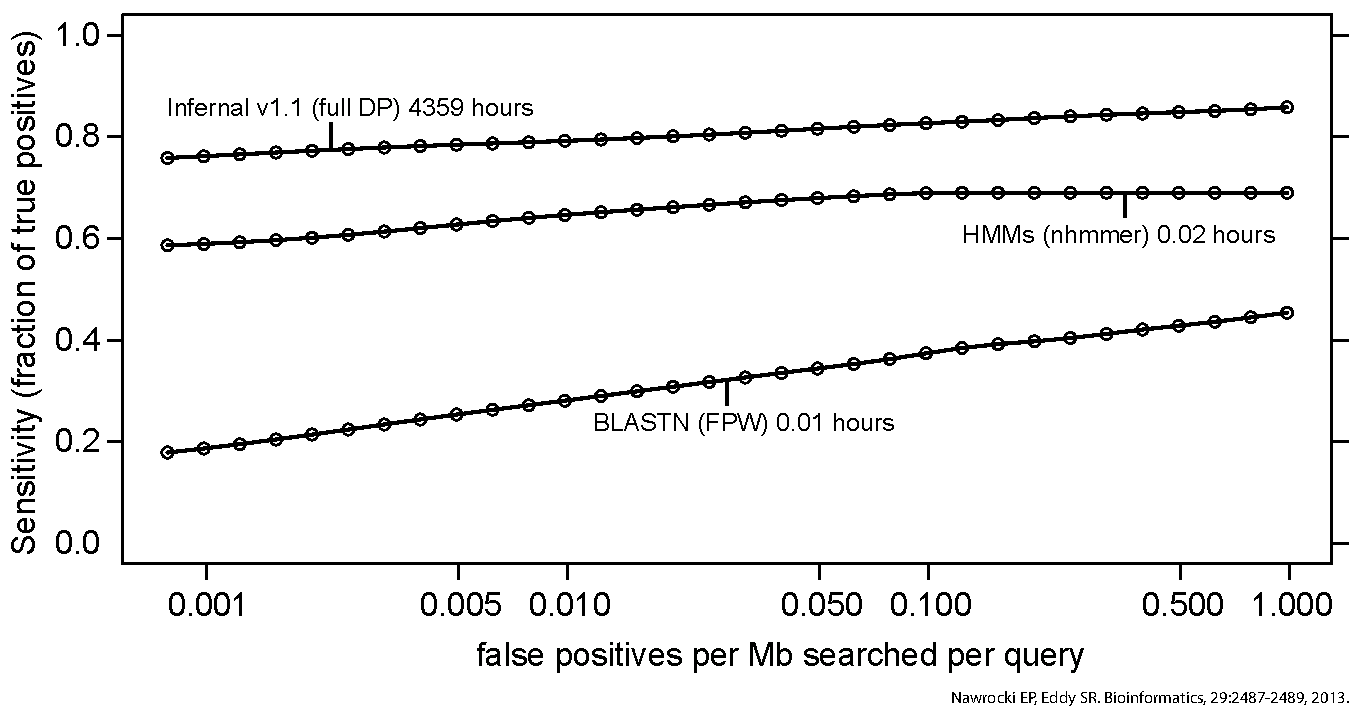
\includegraphics[width=10in]{figs/roc-talk-rcb-2014-1}}

\vfill 
\end{slide}
%%%%%%%%%%%%%%%%%%%%%%%%%%%%%%%%%%%%%%%%%%%%%%%%%%%%%%%%%%%%%%%%%%%%%%
%%%%%%%%%%%%%%%%%%%%%%%%%%%%%%%%%%%%%%%%%%%%%%%%%%%%%%%%%%%%%%%%%%%%%%
\begin{slide}
\begin{center}
\large
\textbf{Filter target database using profile HMMs\footnote{Weinberg,
    Ruzzo, RECOMB, 243-251, 2004; Weinberg, Ruzzo, Bioinformatics,
    22(1) 35-39 2006.}}
\end{center}

\center{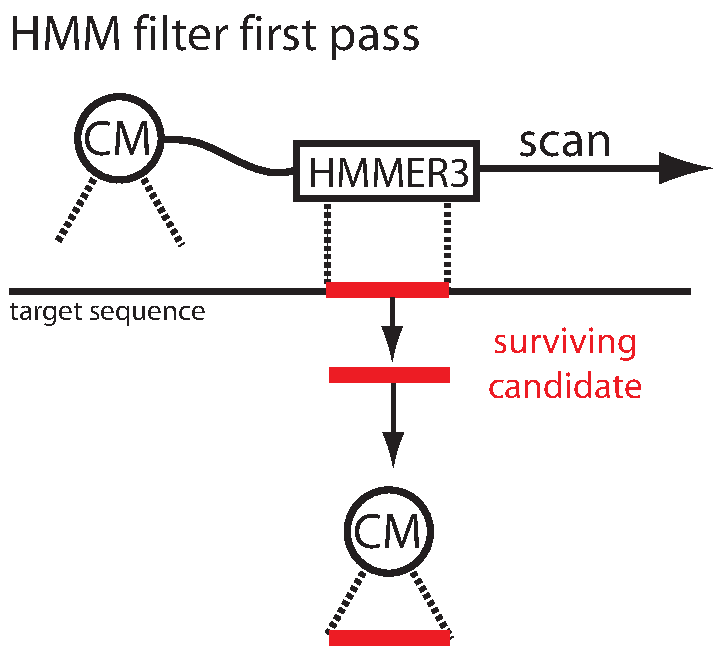
\includegraphics[height=4in]{figs/filter-2014-1}}

\vfill
\end{slide}
%%%%%%%%%%%%%%%%%%%%%%%%%%%%%%%%%%%%%%%%%%%%%%%%%%%%%%%%%%%%%%%%%%%%%%%%%%
\begin{slide}
\begin{center}
\large
\textbf{Filter target database using profile HMMs\footnote{Weinberg,
    Ruzzo, RECOMB, 243-251, 2004; Weinberg, Ruzzo, Bioinformatics,
    22(1) 35-39 2006.}}
\end{center}

\center{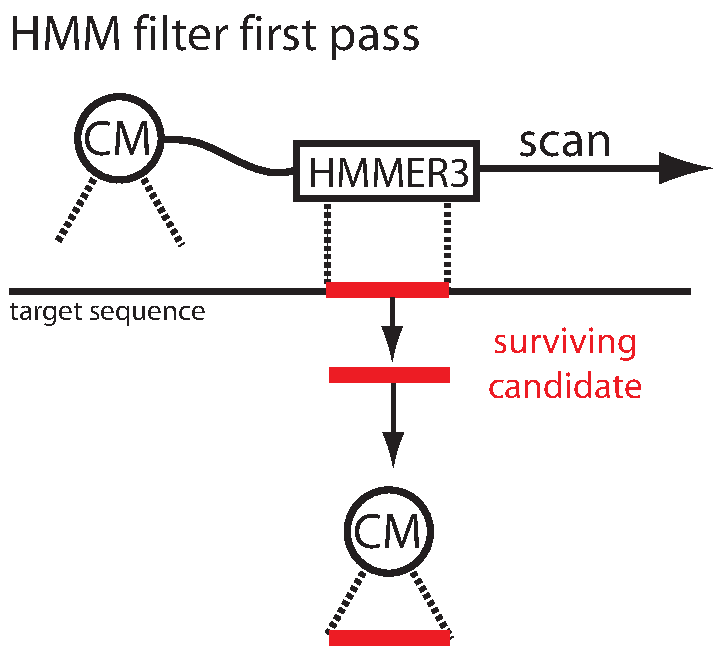
\includegraphics[height=4in]{figs/filter-2014-1}}

\begin{itemize}
\item Even if we filter out 99\% of the database (for up to 100X
  acceleration), searches will still be too slow.
\item CM step needs to be accelerated. 
\end{itemize}

\vfill
\end{slide}
%%%%%%%%%%%%%%%%%%%%%%%%%%%%%%%%%%%%%%%%%%%%%%%%%%%%%%%%%%%%%%%%%%%%%%%%%%
%%%%%%%%%%%%%%%%%%%%%%%%%%%%%%%%%%%%%%%%%%%%%%%%%%%%%%%%%%%%%%%%%%%%%%%%%%
%\begin{slide}
%\begin{center}
%
%\textbf{Accelerating CM alignment step 1: \\ align sequence with HMM}
%
%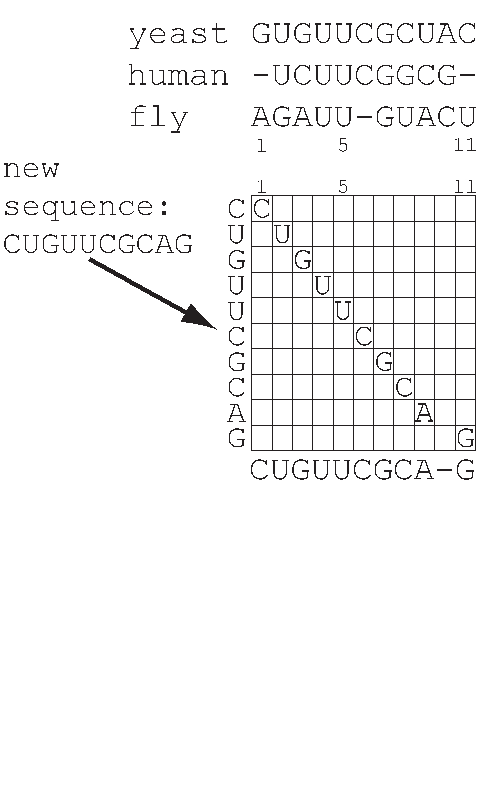
\includegraphics[height=6in]{figs/hmm_alignment2_layer2}
%\end{center}
%
%\vfill
%\end{slide}
%%%%%%%%%%%%%%%%%%%%%%%%%%%%%%%%%%%%%
%%%%%%%%%%%%%%%%%%%%%%%%%%%%%%%%%%%%%%%%%%%%%%%%%%%%%%%%%%%%%%%%%%%%%%%%%%
\begin{slide}
\begin{center}

%\textbf{Accelerating CM alignment step 2: \\ HMM posterior decoding to
%  get confidence estimates}
\textbf{Accelerating CM alignment step 1: \\ HMM posterior decoding to
  get confidence estimates}

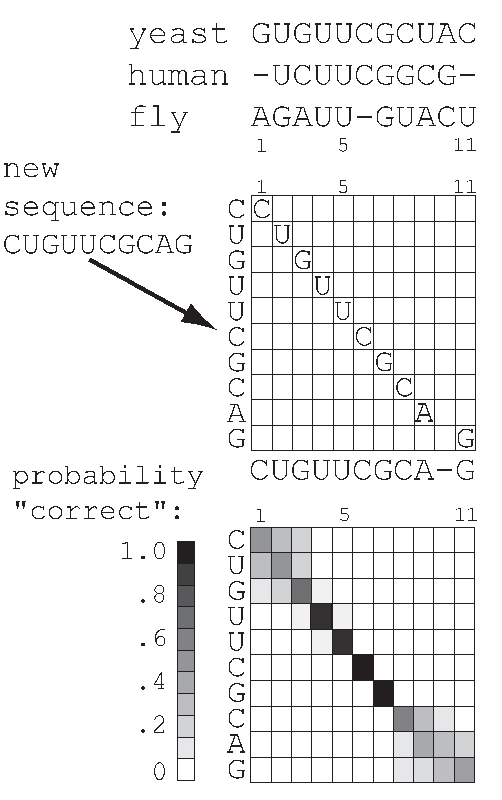
\includegraphics[height=6in]{figs/hmm_alignment2_layer3}
\end{center}

\vfill
\end{slide}
%%%%%%%%%%%%%%%%%%%%%%%%%%%%%%%%%%%%%
\begin{slide}
\begin{center}

\textbf{Accelerating CM alignment step 2: \\ use HMM alignment
  confidence to constrain CM alignment\footnote{M. P. Brown. Proc. Int. Conf. ISMB, 8:57–66, 2000.}}
\end{center}
\medskip
\small
%\begin{itemize}
%\item
%\textbf{main idea:} eliminate potential alignments the HMM tells us are very improbable
%\end{itemize}
\begin{center}
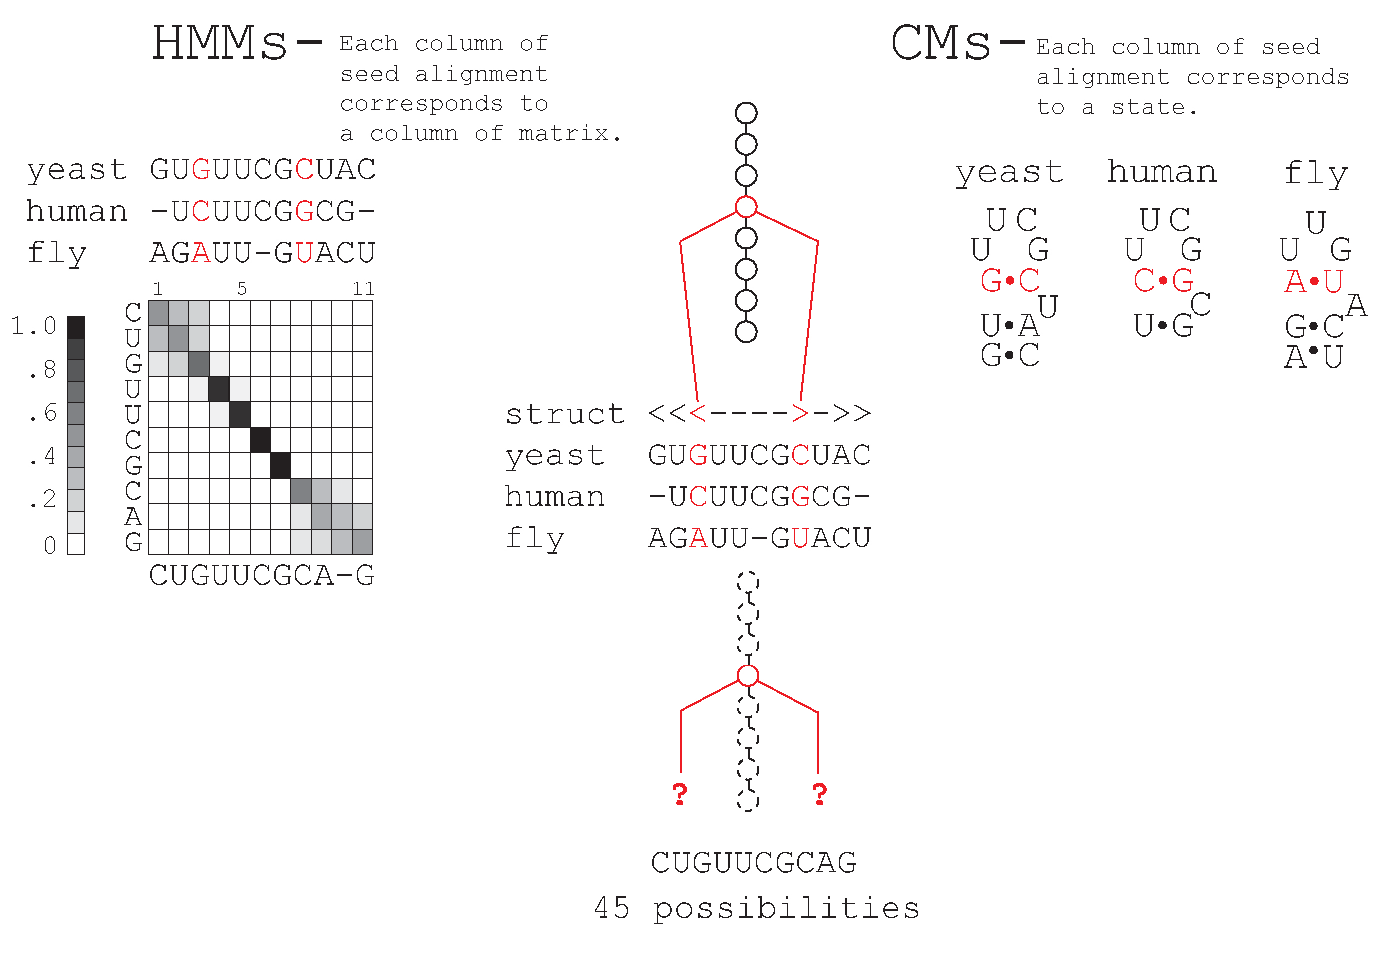
\includegraphics[width=8in]{figs/post_hmm_to_cm_map2_layer14}
\end{center}
\vfill
\end{slide}
%%%%%%%%%%%%%%%%%%%%%%%%%%%%%%%%%%%%%%%%%%%%%%%%%%%%%%%%%%%%%%%%%%%%%%
\begin{slide}
\begin{center}

\textbf{Accelerating CM alignment step 2: \\ use HMM alignment
  confidence to constrain CM alignment\footnote{M. P. Brown. Proc. Int. Conf. ISMB, 8:57–66, 2000.}}
\end{center}
\medskip
\small
%\begin{itemize}
%\item
%\textbf{main idea:} eliminate potential alignments the HMM tells us are very improbable
%\end{itemize}
\begin{center}
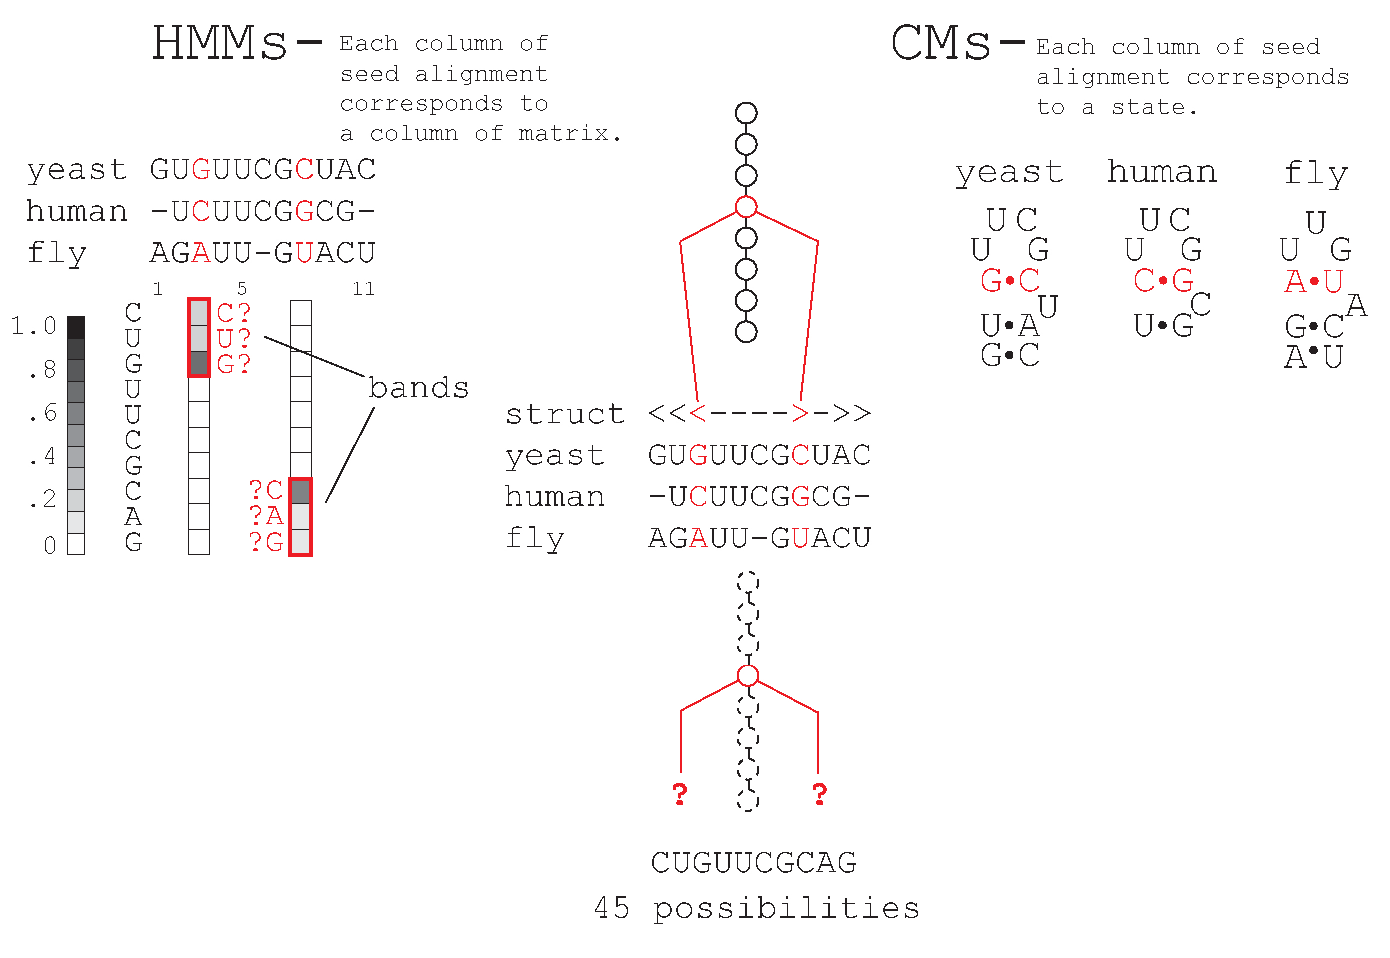
\includegraphics[width=8in]{figs/post_hmm_to_cm_map2_layer15}
\end{center}
\vfill
\end{slide}
%%%%%%%%%%%%%%%%%%%%%%%%%%%%%%%%%%%%%%%%%%%%%%%%%%%%%%%%%%%%%%%%%%%%%%%%%%
\begin{slide}
\begin{center}

\textbf{Accelerating CM alignment step 3: \\ use HMM alignment
  confidence to constrain CM alignment\footnote{M. P. Brown. Proc. Int. Conf. ISMB, 8:57–66, 2000.}}
\end{center}
\medskip
\small
%\begin{itemize}
%\item
%\textbf{main idea:} eliminate potential alignments the HMM tells us are very improbable
%\end{itemize}
\begin{center}
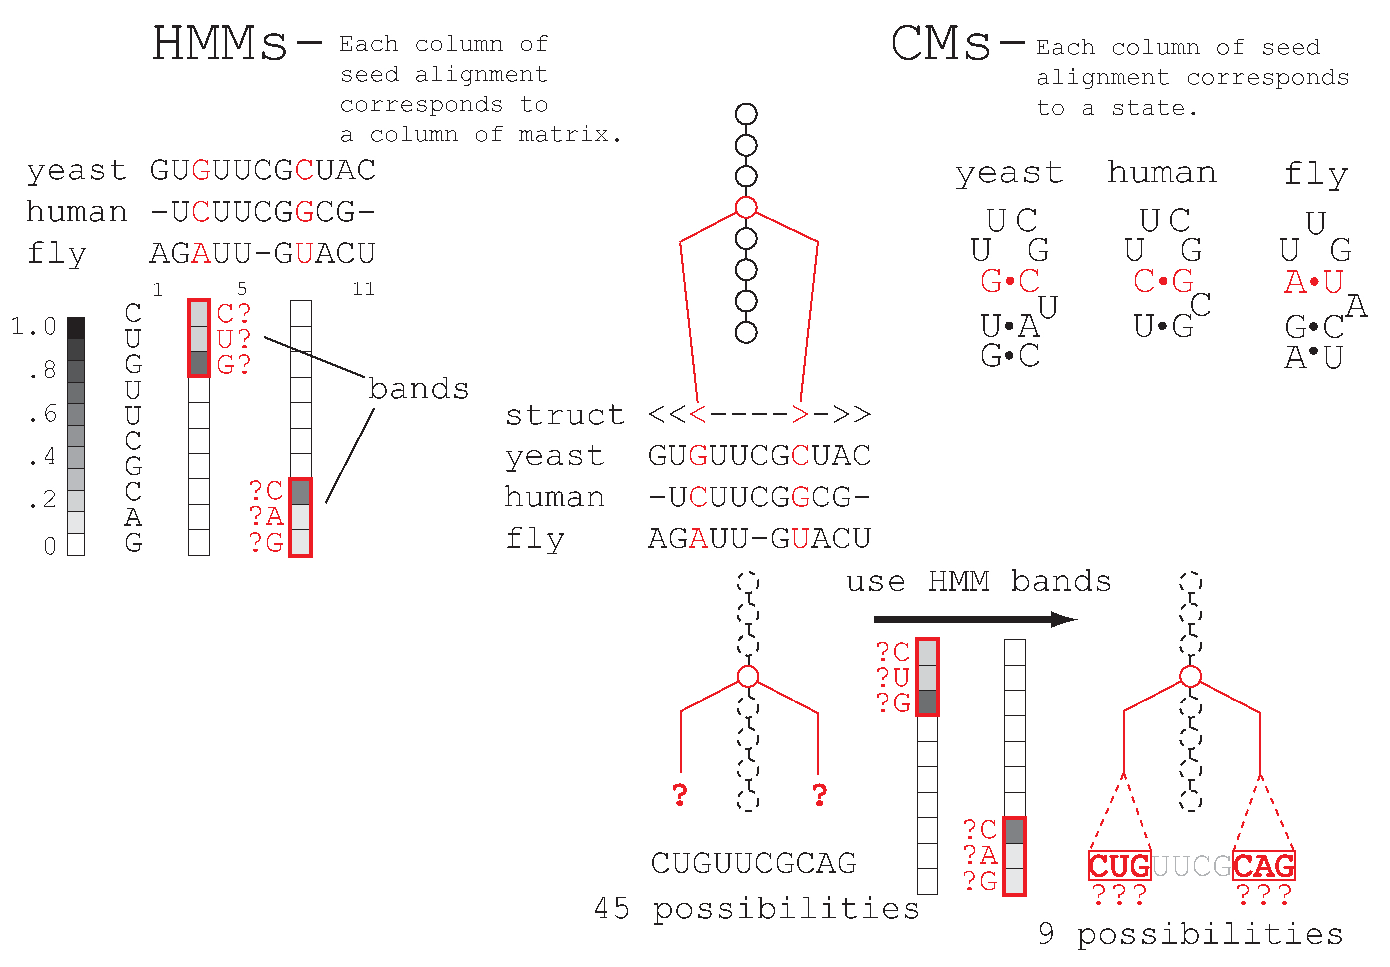
\includegraphics[width=8in]{figs/post_hmm_to_cm_map2_layer16}
\end{center}
\vfill
\end{slide}
%%%%%%%%%%%%%%%%%%%%%%%%%%%%%%%%%%%%%%%%%%%%%%%%%%%%%%%%%%%%%%%%%%%%%%
\begin{slide}
\center{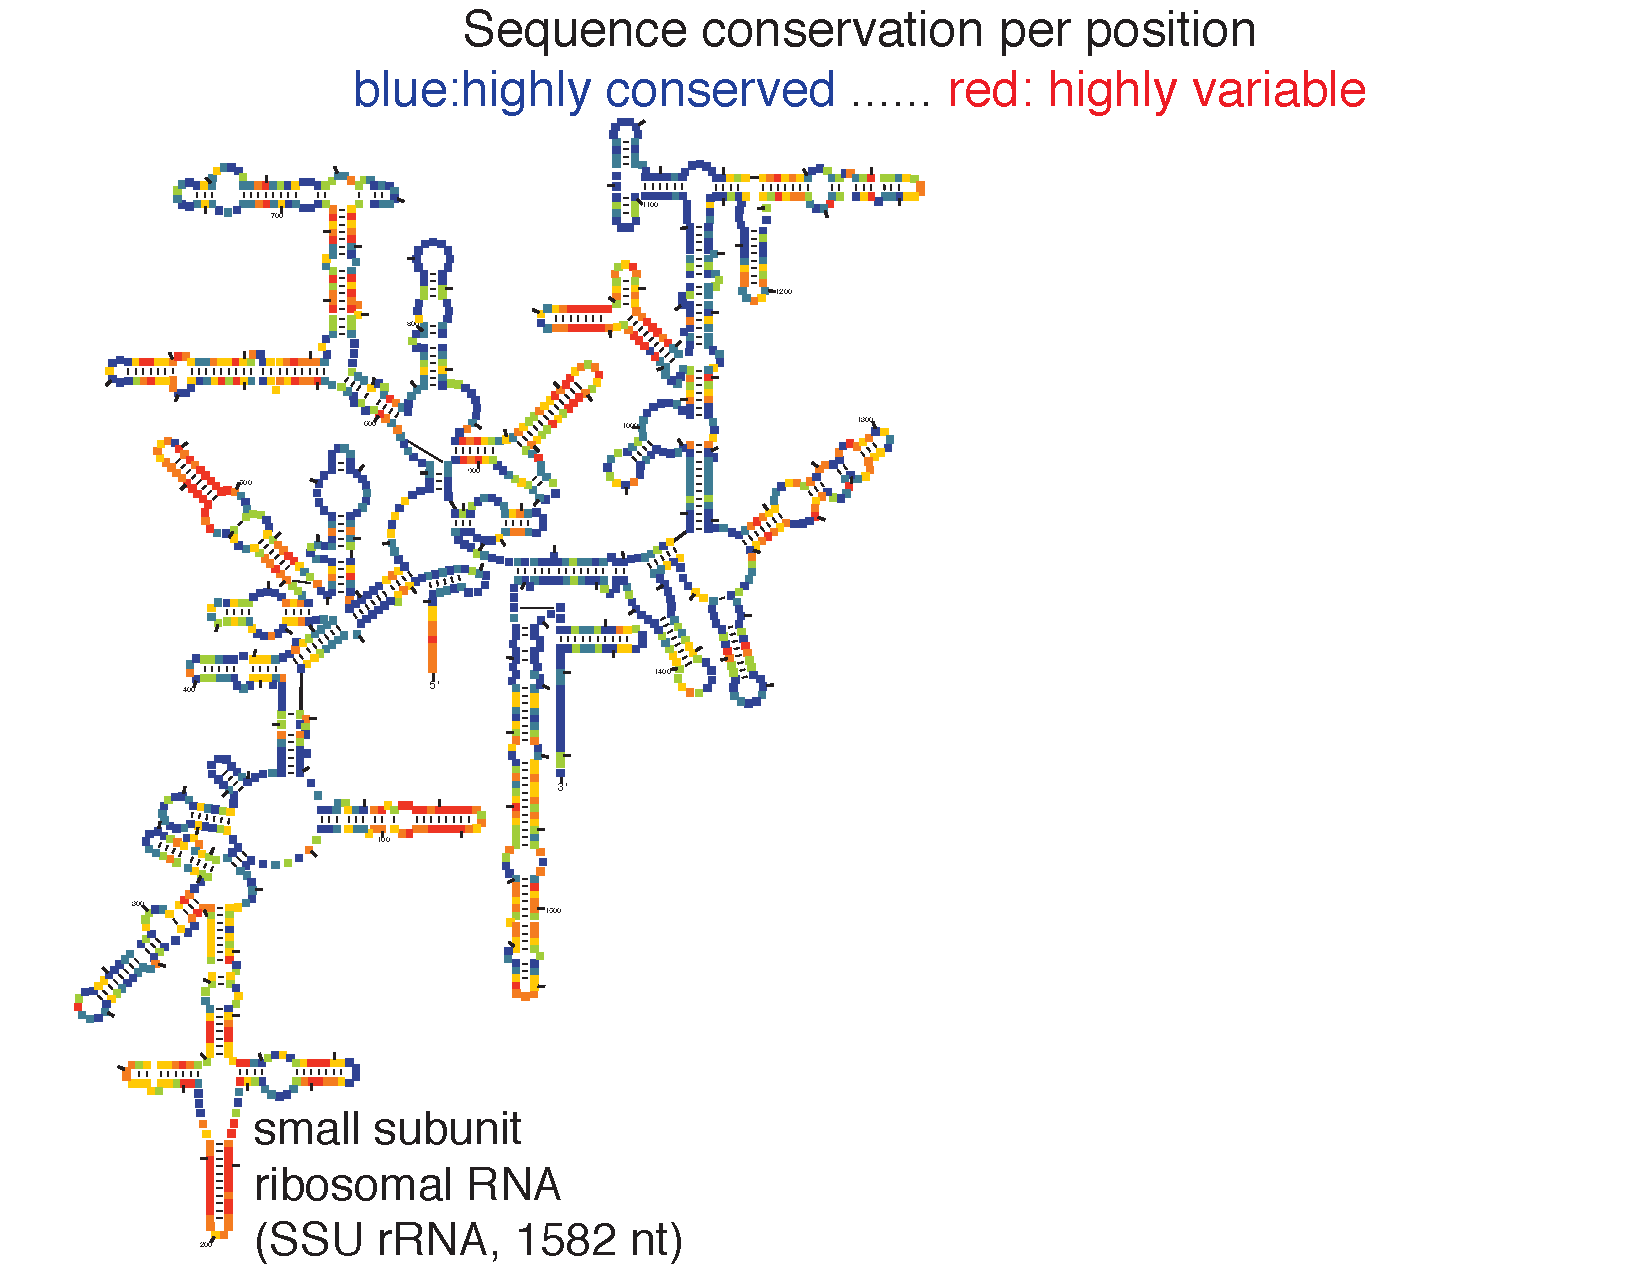
\includegraphics[width=10.5in]{figs/16s-5s-trna-info-16sonly}}
\end{slide}
%%%%%%%%%%%%%%%%%%%%%%%%%%%%%%%%%%%%%%%%%%%%%%%%%%%%%%%%%%%%%%%%%%%%%%
\begin{slide}
\center{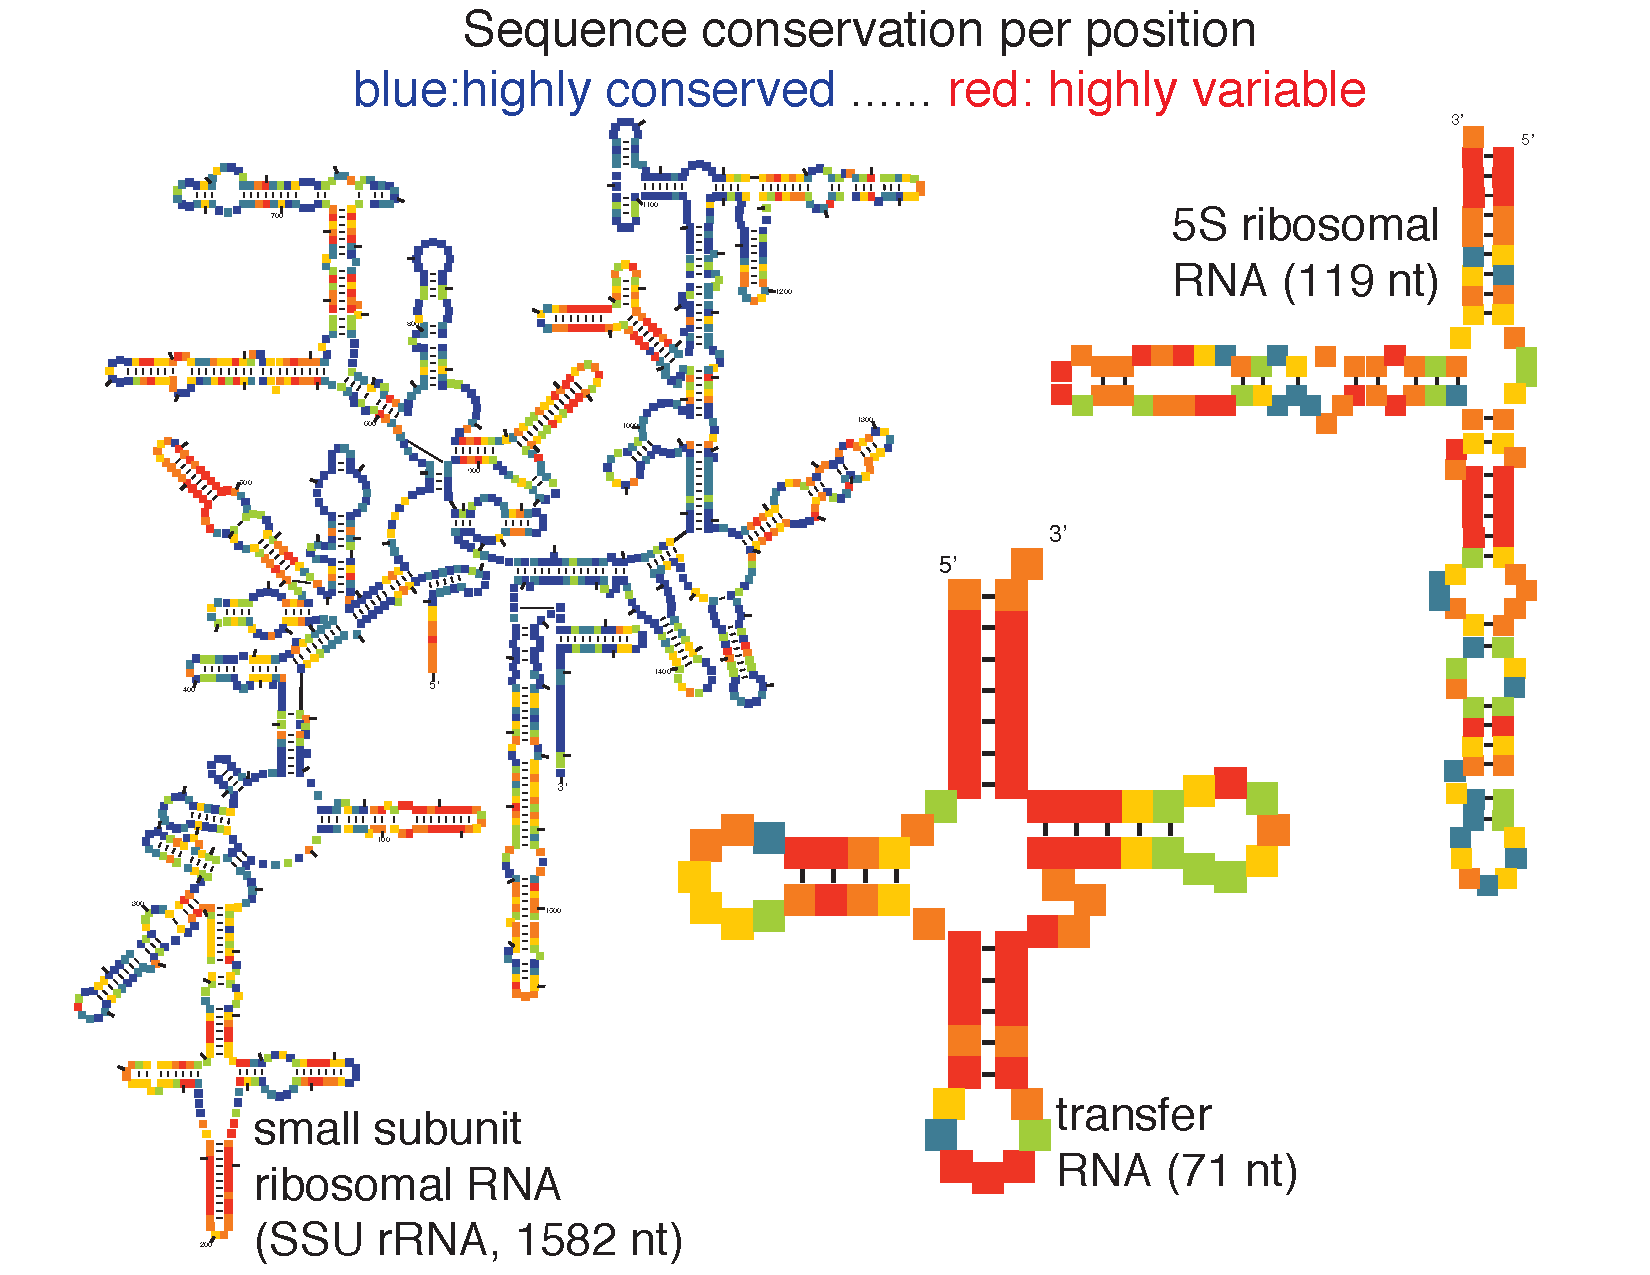
\includegraphics[width=10.5in]{figs/16s-5s-trna-info}}
\end{slide}
%%%%%%%%%%%%%%%%%%%%%%%%%%%%%%%%%%%%%%%%%%%%%%%%%%%%%%%%%%%%%%%%%%%%
\begin{slide}
\begin{center}
\large
\textbf{Use HMMs as filters and to constrain CM alignment}
\end{center}

\center{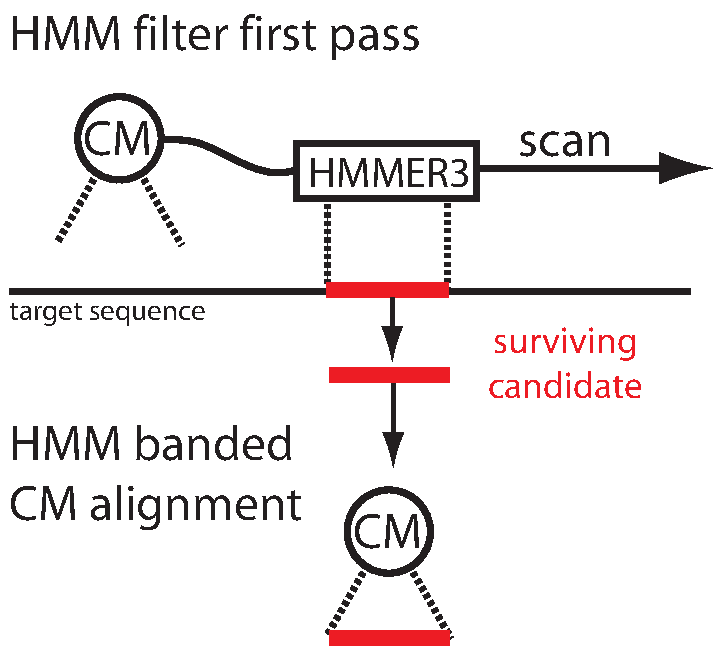
\includegraphics[height=5in]{figs/filter-2014-2}}

\vfill
\end{slide}
%%%%%%%%%%%%%%%%%%%%%%%%%%%%%%%%%%%%%%%%%%%%%%%%%%%%%%%%%%%%%%%%%%%%%%%%%%
\begin{slide}
\begin{center}

\textbf{HMM-based acceleration makes Infernal 10,000 times faster}

\end{center}
\medskip

\center{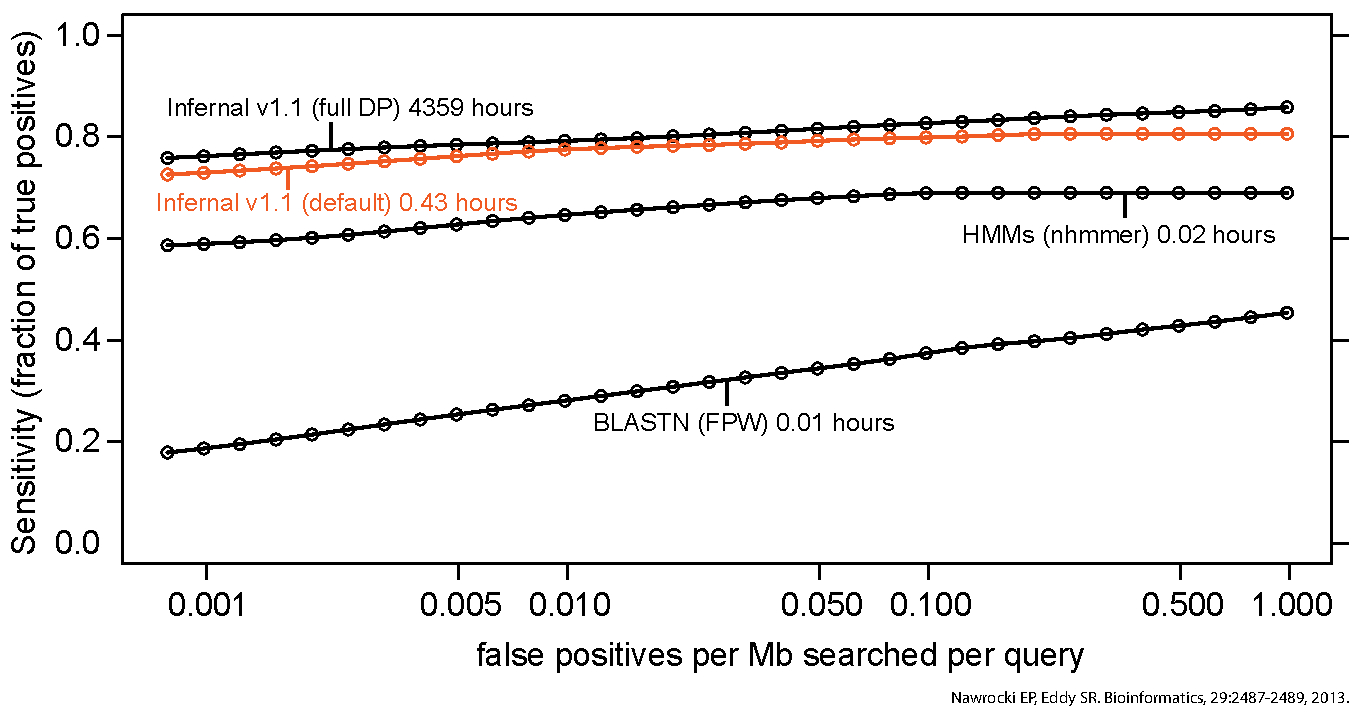
\includegraphics[width=10in]{figs/roc-talk-rcb-2014-2}}

\vfill 
\end{slide}
%%%%%%%%%%%%%%%%%%%%%%%%%%%%%%%%%%%%%%%%%%%%%%%%%%%%%%%%%%%%%%%%%%%%%%
\begin{slide}
\begin{center}
\textbf{Applications of CMs}
\end{center}

\small
\begin{itemize}
\item homology search/alignment: Infernal,
  COVE, Rfam\footnote{Kalvari et al., NAR, 2018, 46(D1), D335-D342.},
  Alternal\footnote{S. Janssen and R. Giegerich. BMC Bioinformatics
    2015, 16:178}, RNATOPS\footnote{Z. Huang et al, 
    Bioinformatics, 24(20), 2281-2287, 2008.}
    
\item RNA discovery: CMfinder\footnote{Z. Yao, Z. Weinberg, W. L. Ruzzo,
  Bioinformatics 2006, 22(4), 445-452.}, 
  Zasha's pipeline(s)\footnote{
    Z. Weinberg et al., NAR, 2017. 45(18), 10811–10823,
    Z. Weinberg et al. Genome Biol, 2010. 11(3), R31.,
    Z. Weinberg et al., NAR, 2007. 35(14), 4809-4819}
\item structure comparison: CMCompare\footnote{F. Eggenhofer et al.,
  NAR, 2013, 41(W1),  W499–W503.,
  C. H. zu Siederdissen, and
  I. L. Hofacker Bioinformatics, 2010. 26(18), i453-i459.}
\item family-specific programs/databases: 
\begin{itemize}
\item tRNAscan-SE\footnote{T. M. Lowe, S. R. Eddy. NAR,
    25:955-964, 1997.}, 
\item 16S/18S rRNA alignment: Ribosomal Database Project
  (RDP) and SSU-ALIGN\footnote{J. R. Cole et al., NAR, 2014, 42D, D633-D642; E. P. Nawrocki. PhD
  Thesis: 2009, Wash U School of Med}
\item bacterial terminator identification: RNIE\footnote{P.P. Gardner
  et al. NAR, 2011, 39(14), 5845-5852.}
\end{itemize}
\end{itemize}

\vfill 
\end{slide}
%%%%%%%%%%%%%%%%%%%%%%%%%%%%%%%%%%%%%%%%%%%%%%%%%%%%%%%%%%%%%%%%%%%%%%
\begin{slide}
\begin{center}
\textbf{Infernal 1.1 finds 11,000 new group I intron candidates}
\end{center}

%\center{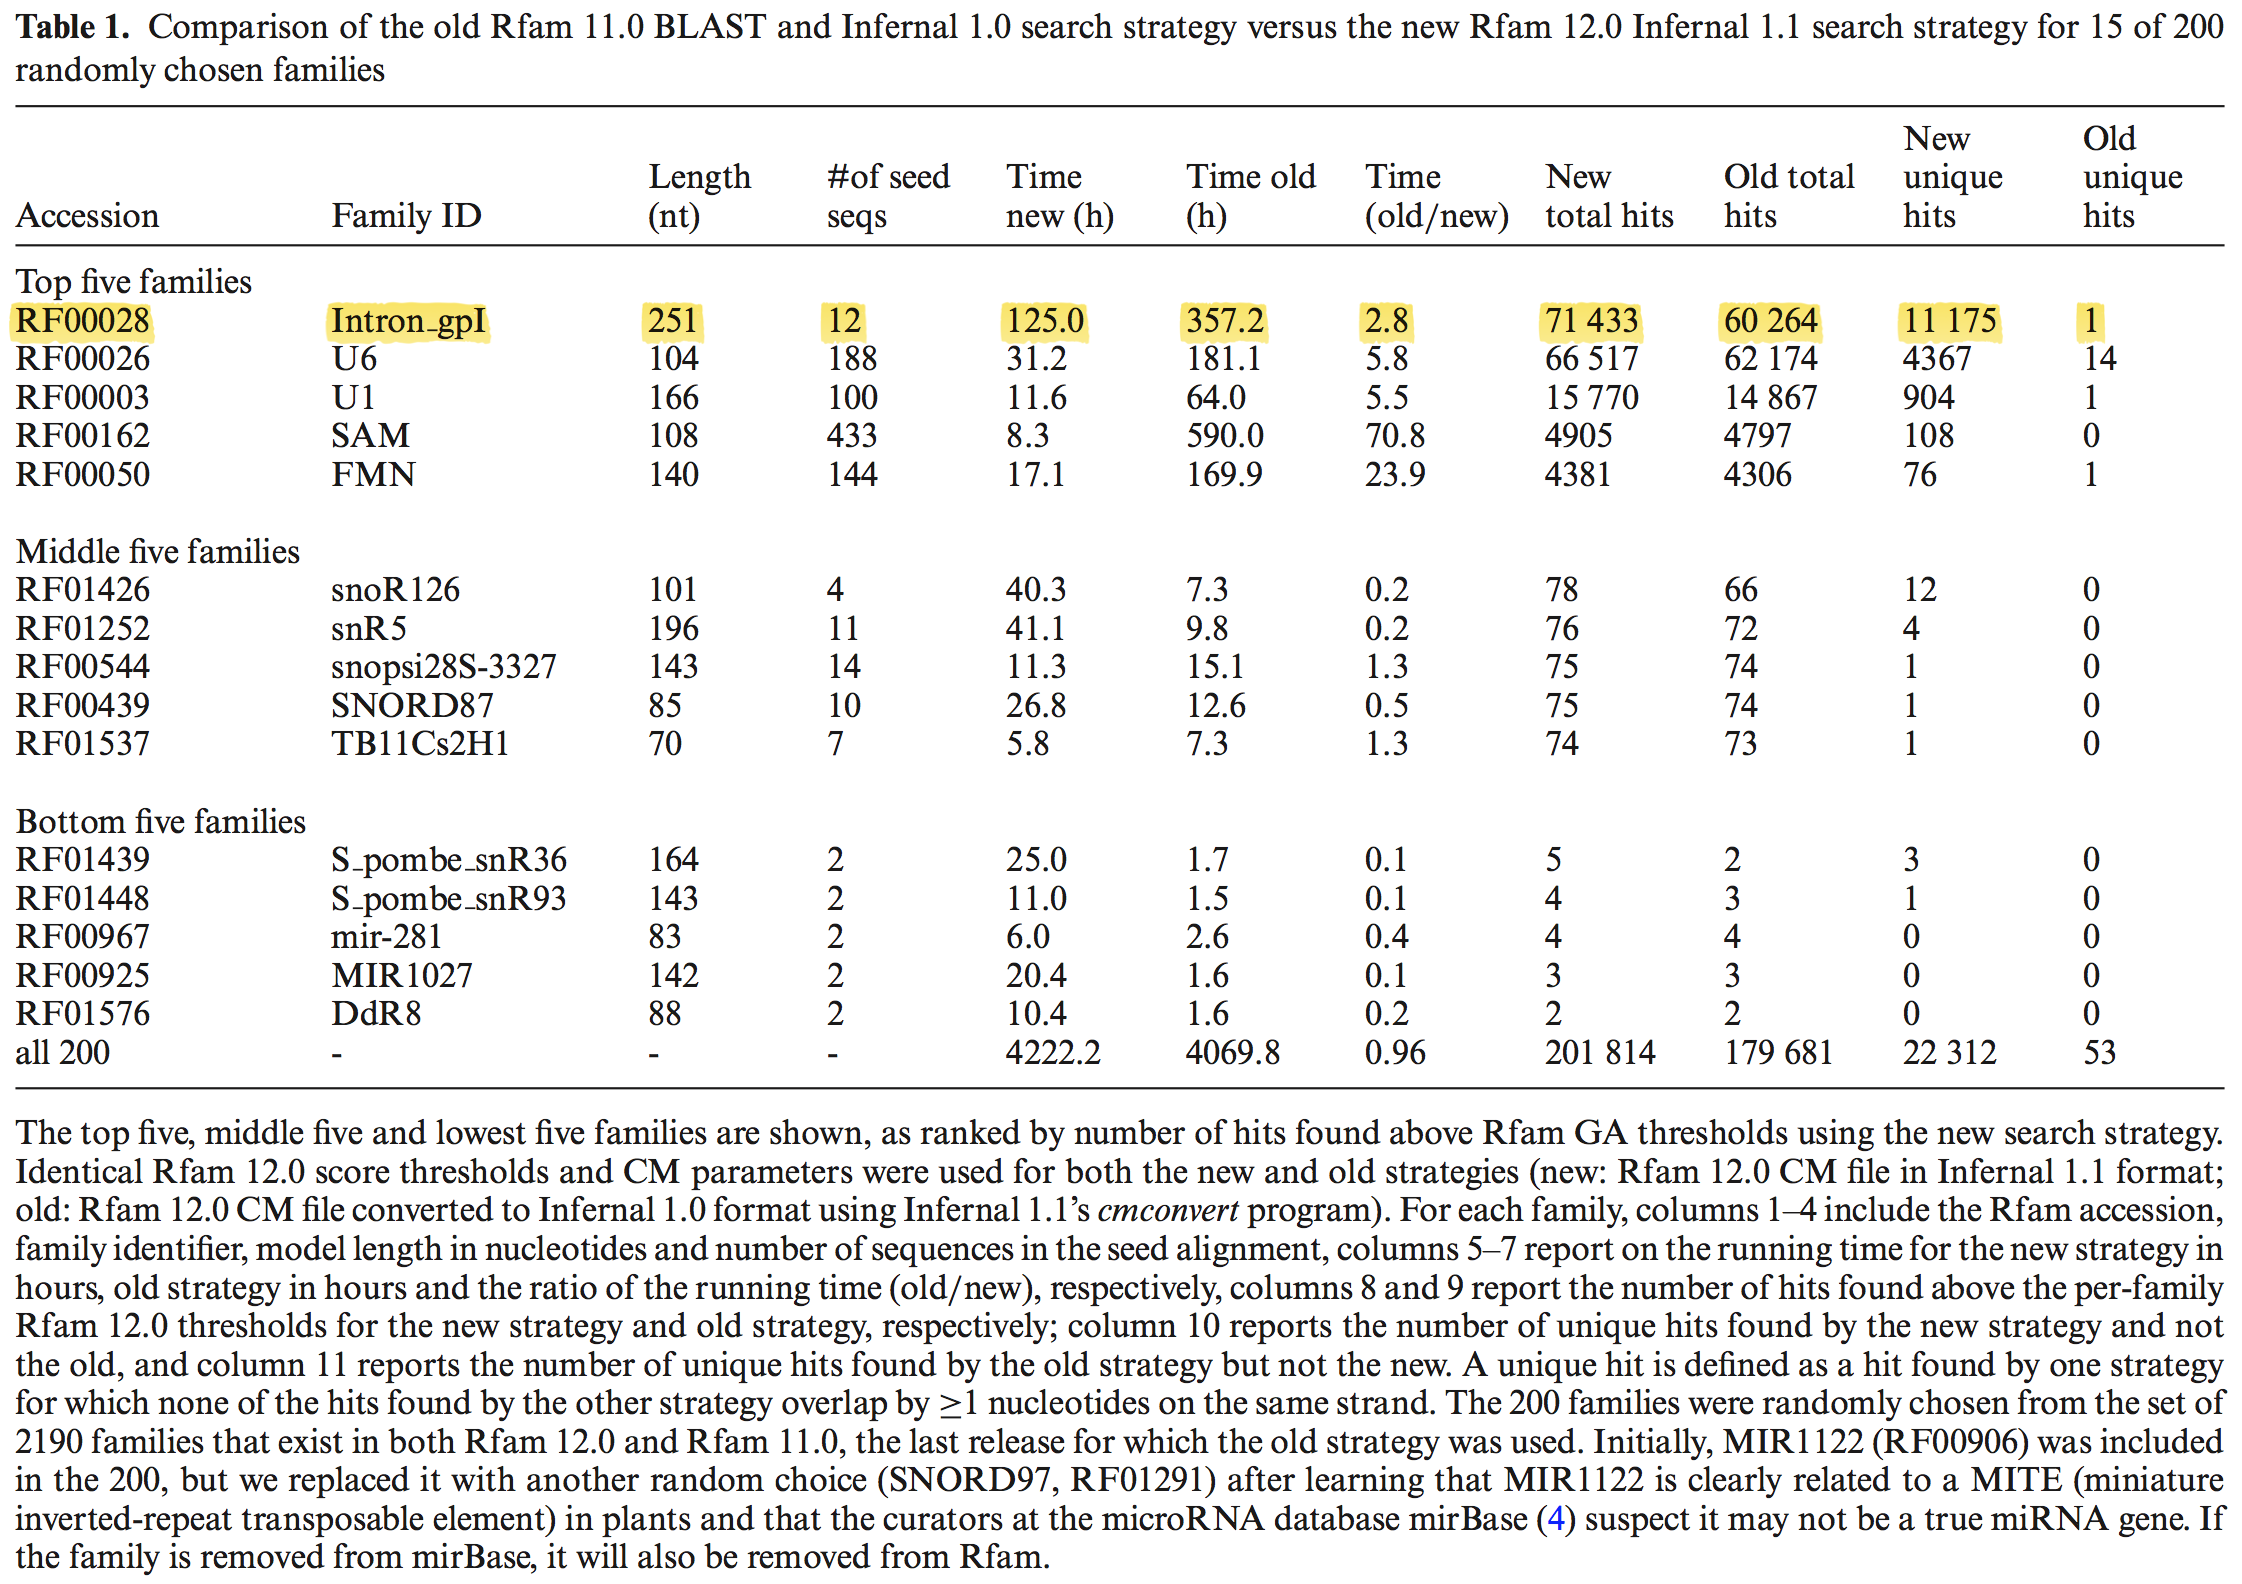
\includegraphics[width=10.5in]{figs/rfam-nar-table1-published-gp1i-yellow}}
\center{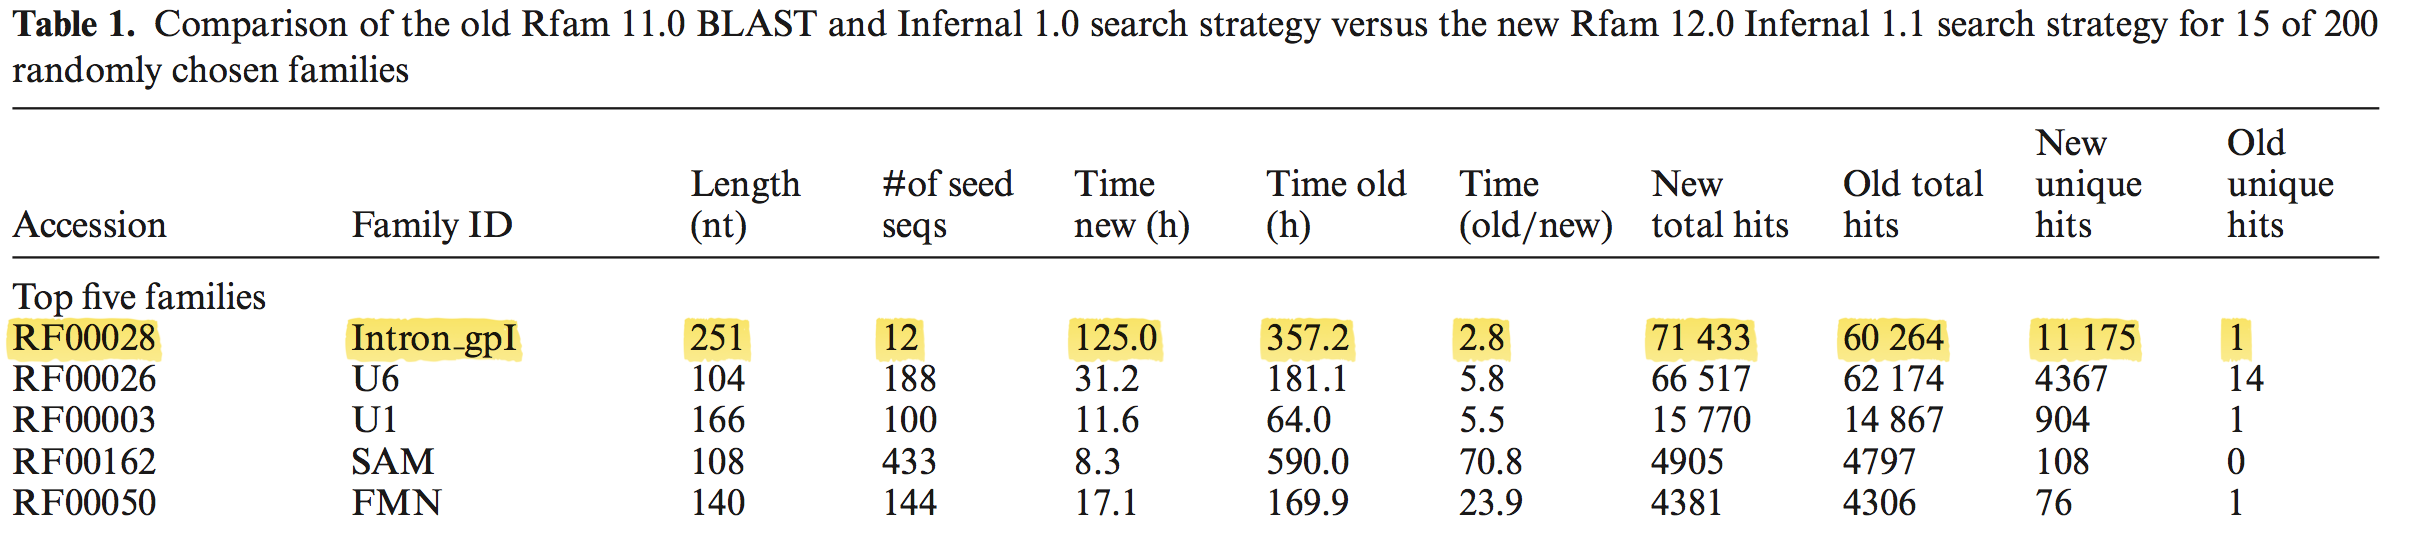
\includegraphics[width=10.5in]{figs/rfam-nar-table1-published-gp1i-yellow-top5only}}

\vfill
\end{slide}
%%%%%%%%%%%%%%%%%%%%%%%%%%%%%%%%%%%%%%%%%%%%%%%%%%%%%%%%%%%%%%%%%%%%%%%%%%
%%%%%%%%%%%%%%%%%%%%%%%%%%%%%%%%%%%%%%%%%%%%%%%%%%%%%%%%%%%%%%%%%%%%%%
\begin{slide}
\begin{center}
\textbf{Group I catalytic introns}
\end{center}
%
\small
\begin{itemize}
\item self splicing ribozymes found in lower eukaryotes, higher
  plants, bacteria and bacteriophages
%\item core secondary structure (modeled by Rfam) consists of 9 paired
%  regions
\item often have ORFs (homing endonucleases) inserted in loop regions
\item genes they are found in:
\begin {itemize}
\item bacteria and mitochondria and chloroplast of lower euks: rRNA, mRNA, and tRNAs
\item higher plants mitochondria and chloroplast: a few tRNA and mRNA genes
\item nuclear lower eukaryotic genomes: only rRNA
%\item Gram positive bacteriophages: widely distributed
%\item Gram negative bacteriophages: T4, T-even and T7-like
\end{itemize}
\end{itemize}

%\center{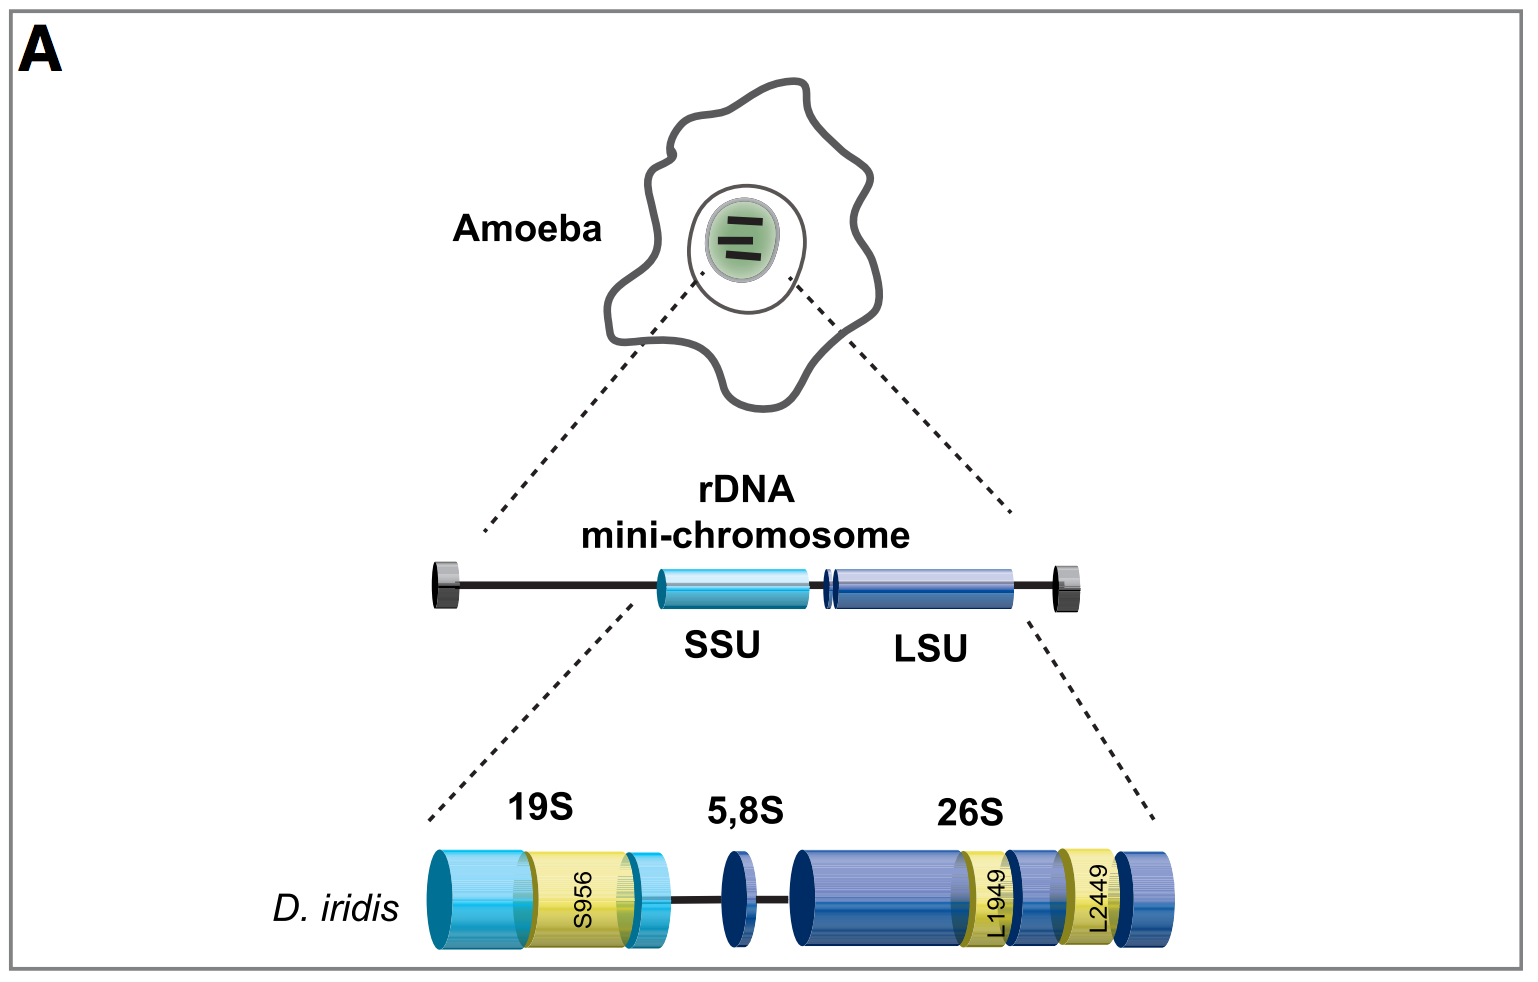
\includegraphics[height=4in]{figs/gp1-schematic-small.png}}
\center{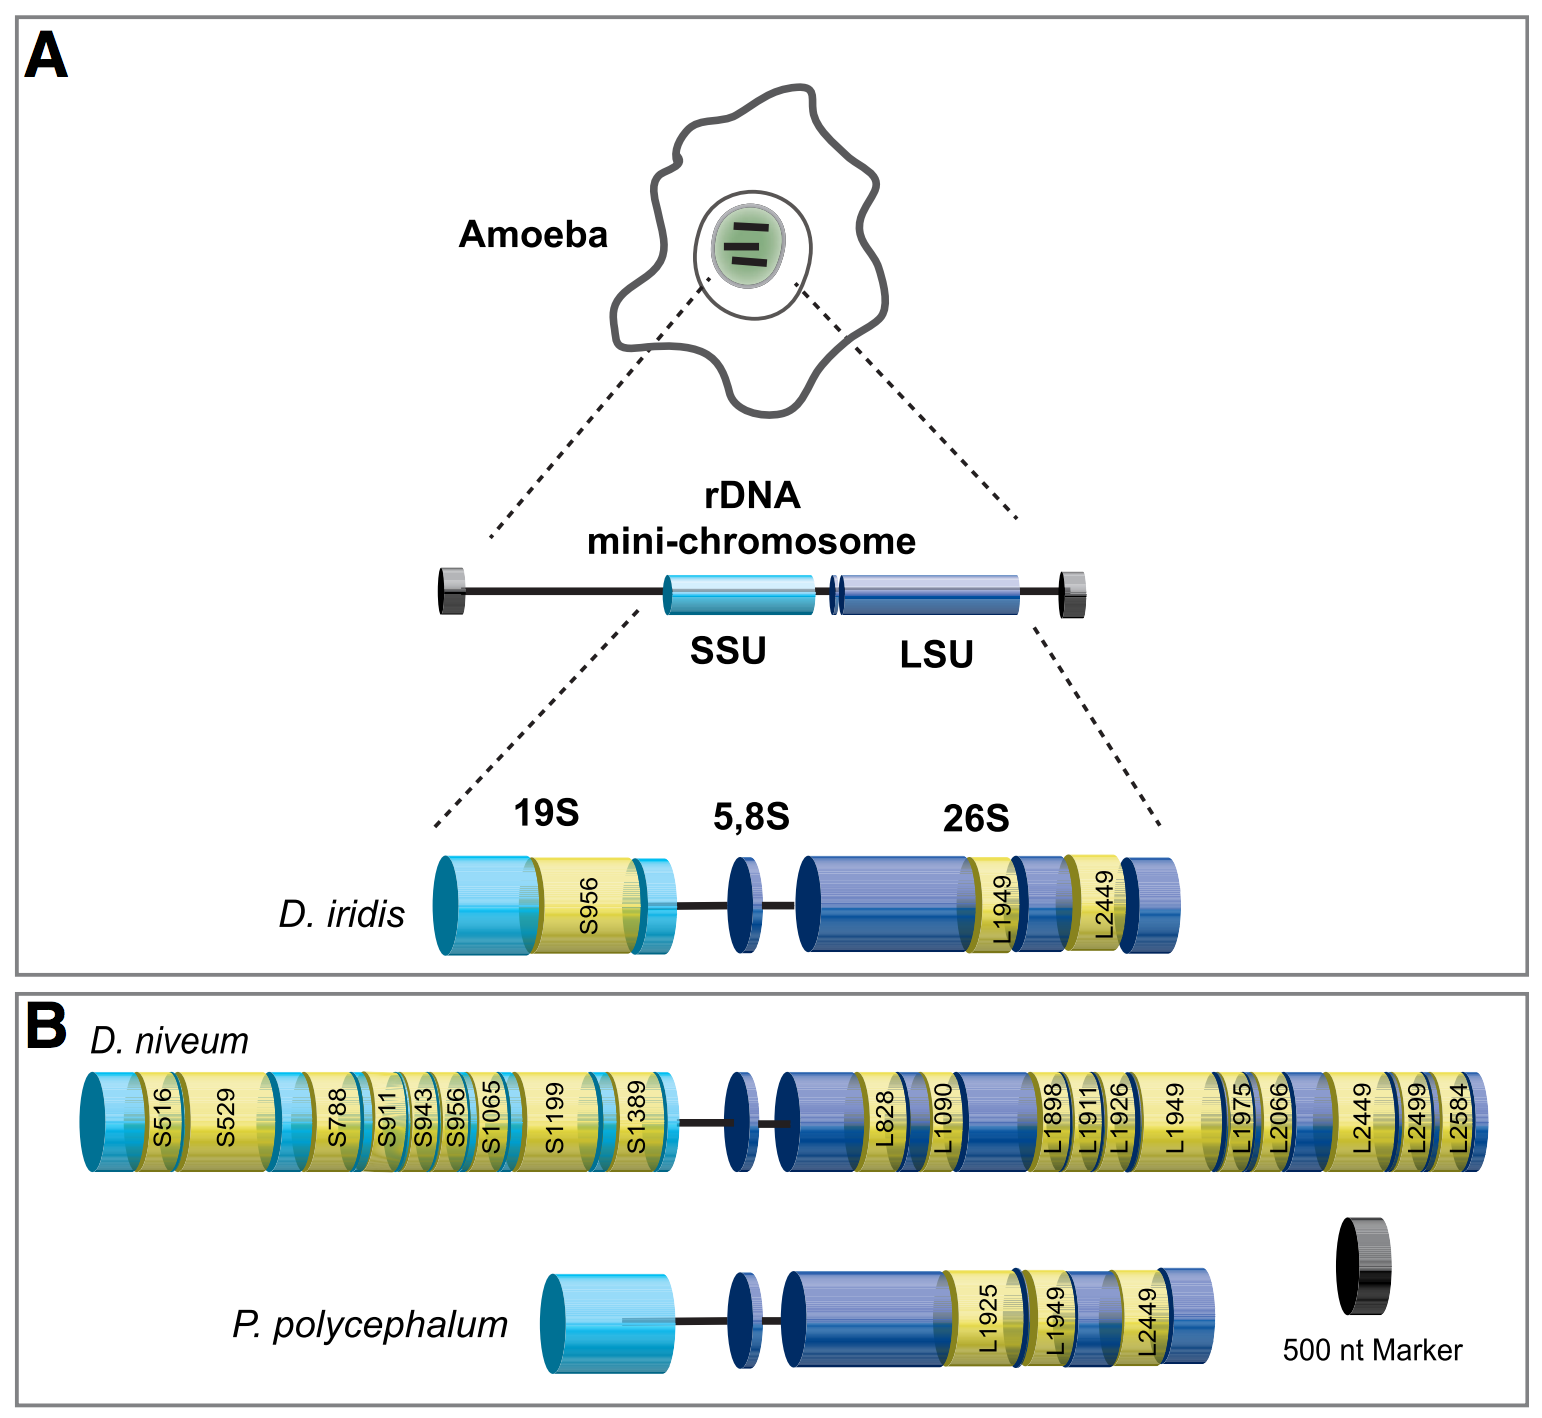
\includegraphics[height=4.5in]{figs/gp1-schematic-big.png}}


\vfill
\end{slide}
%%%%%%%%%%%%%%%%%%%%%%%%%%%%%%%%%%%%%%%%%%%%%%%%%%%%%%%%%%%%%%%%%%%%%%%%%%
\begin{slide}
\center{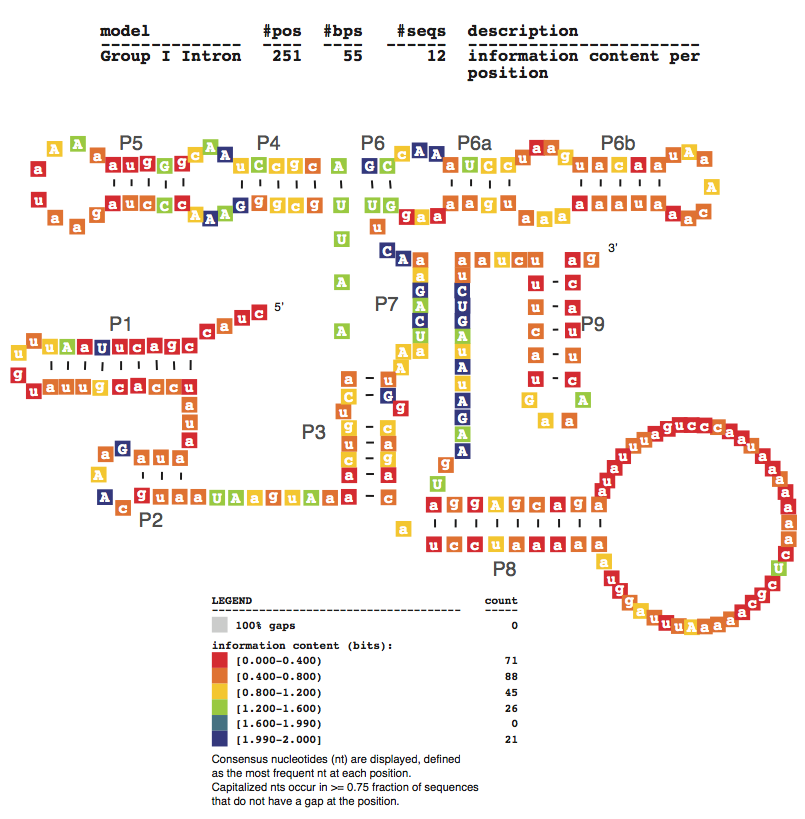
\includegraphics[height=8in]{figs/RF00028-ss-info-ss-1}}
\vfill
\end{slide}
%%%%%%%%%%%%%%%%%%%%%%%%%%%%%%%%%%%%%%%%%%%%%%%%%%%%%%%%%%%%%%%%%%%%%%%%%%
\begin{slide}
\center{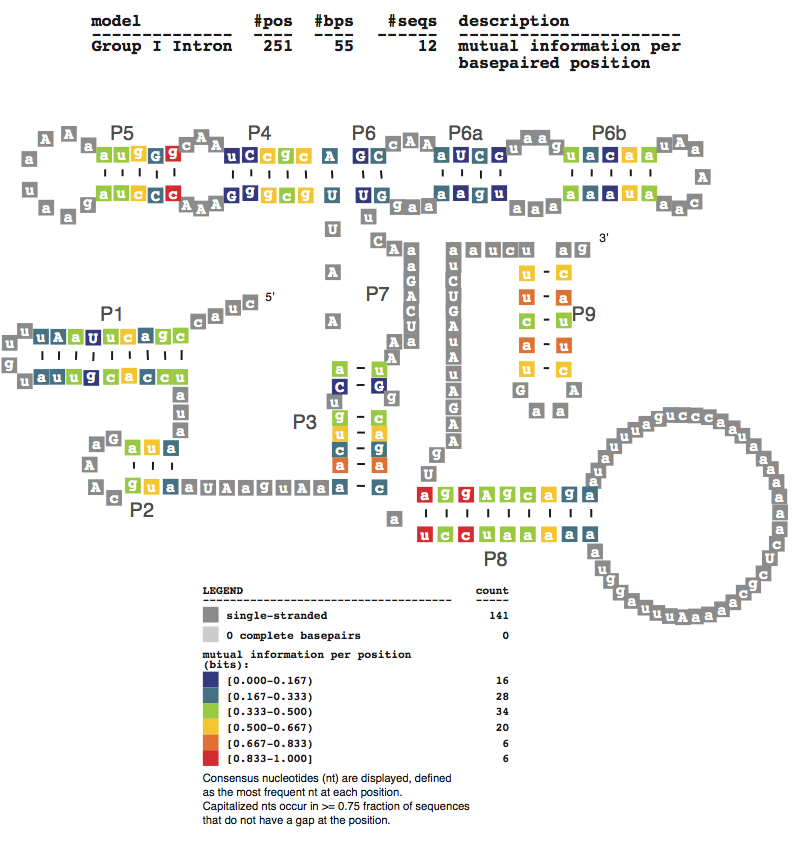
\includegraphics[height=8in]{figs/RF00028-ss-mutinfo-ss-1}}
\vfill
\end{slide}
%%%%%%%%%%%%%%%%%%%%%%%%%%%%%%%%%%%%%%%%%%%%%%%%%%%%%%%%%%%%%%%%%%%%%%%%%%
\begin{slide}
\begin{center}
\small
\textbf{GISSD\footnote{Y. Zhou et. al, NAR, 2008. 36(suppl
    1), D31-D37.}: Group I Intron Sequence and Structure Database}
\end{center}

\center{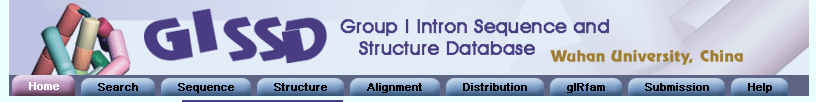
\includegraphics[width=8in]{figs/gissd-banner}}

\center{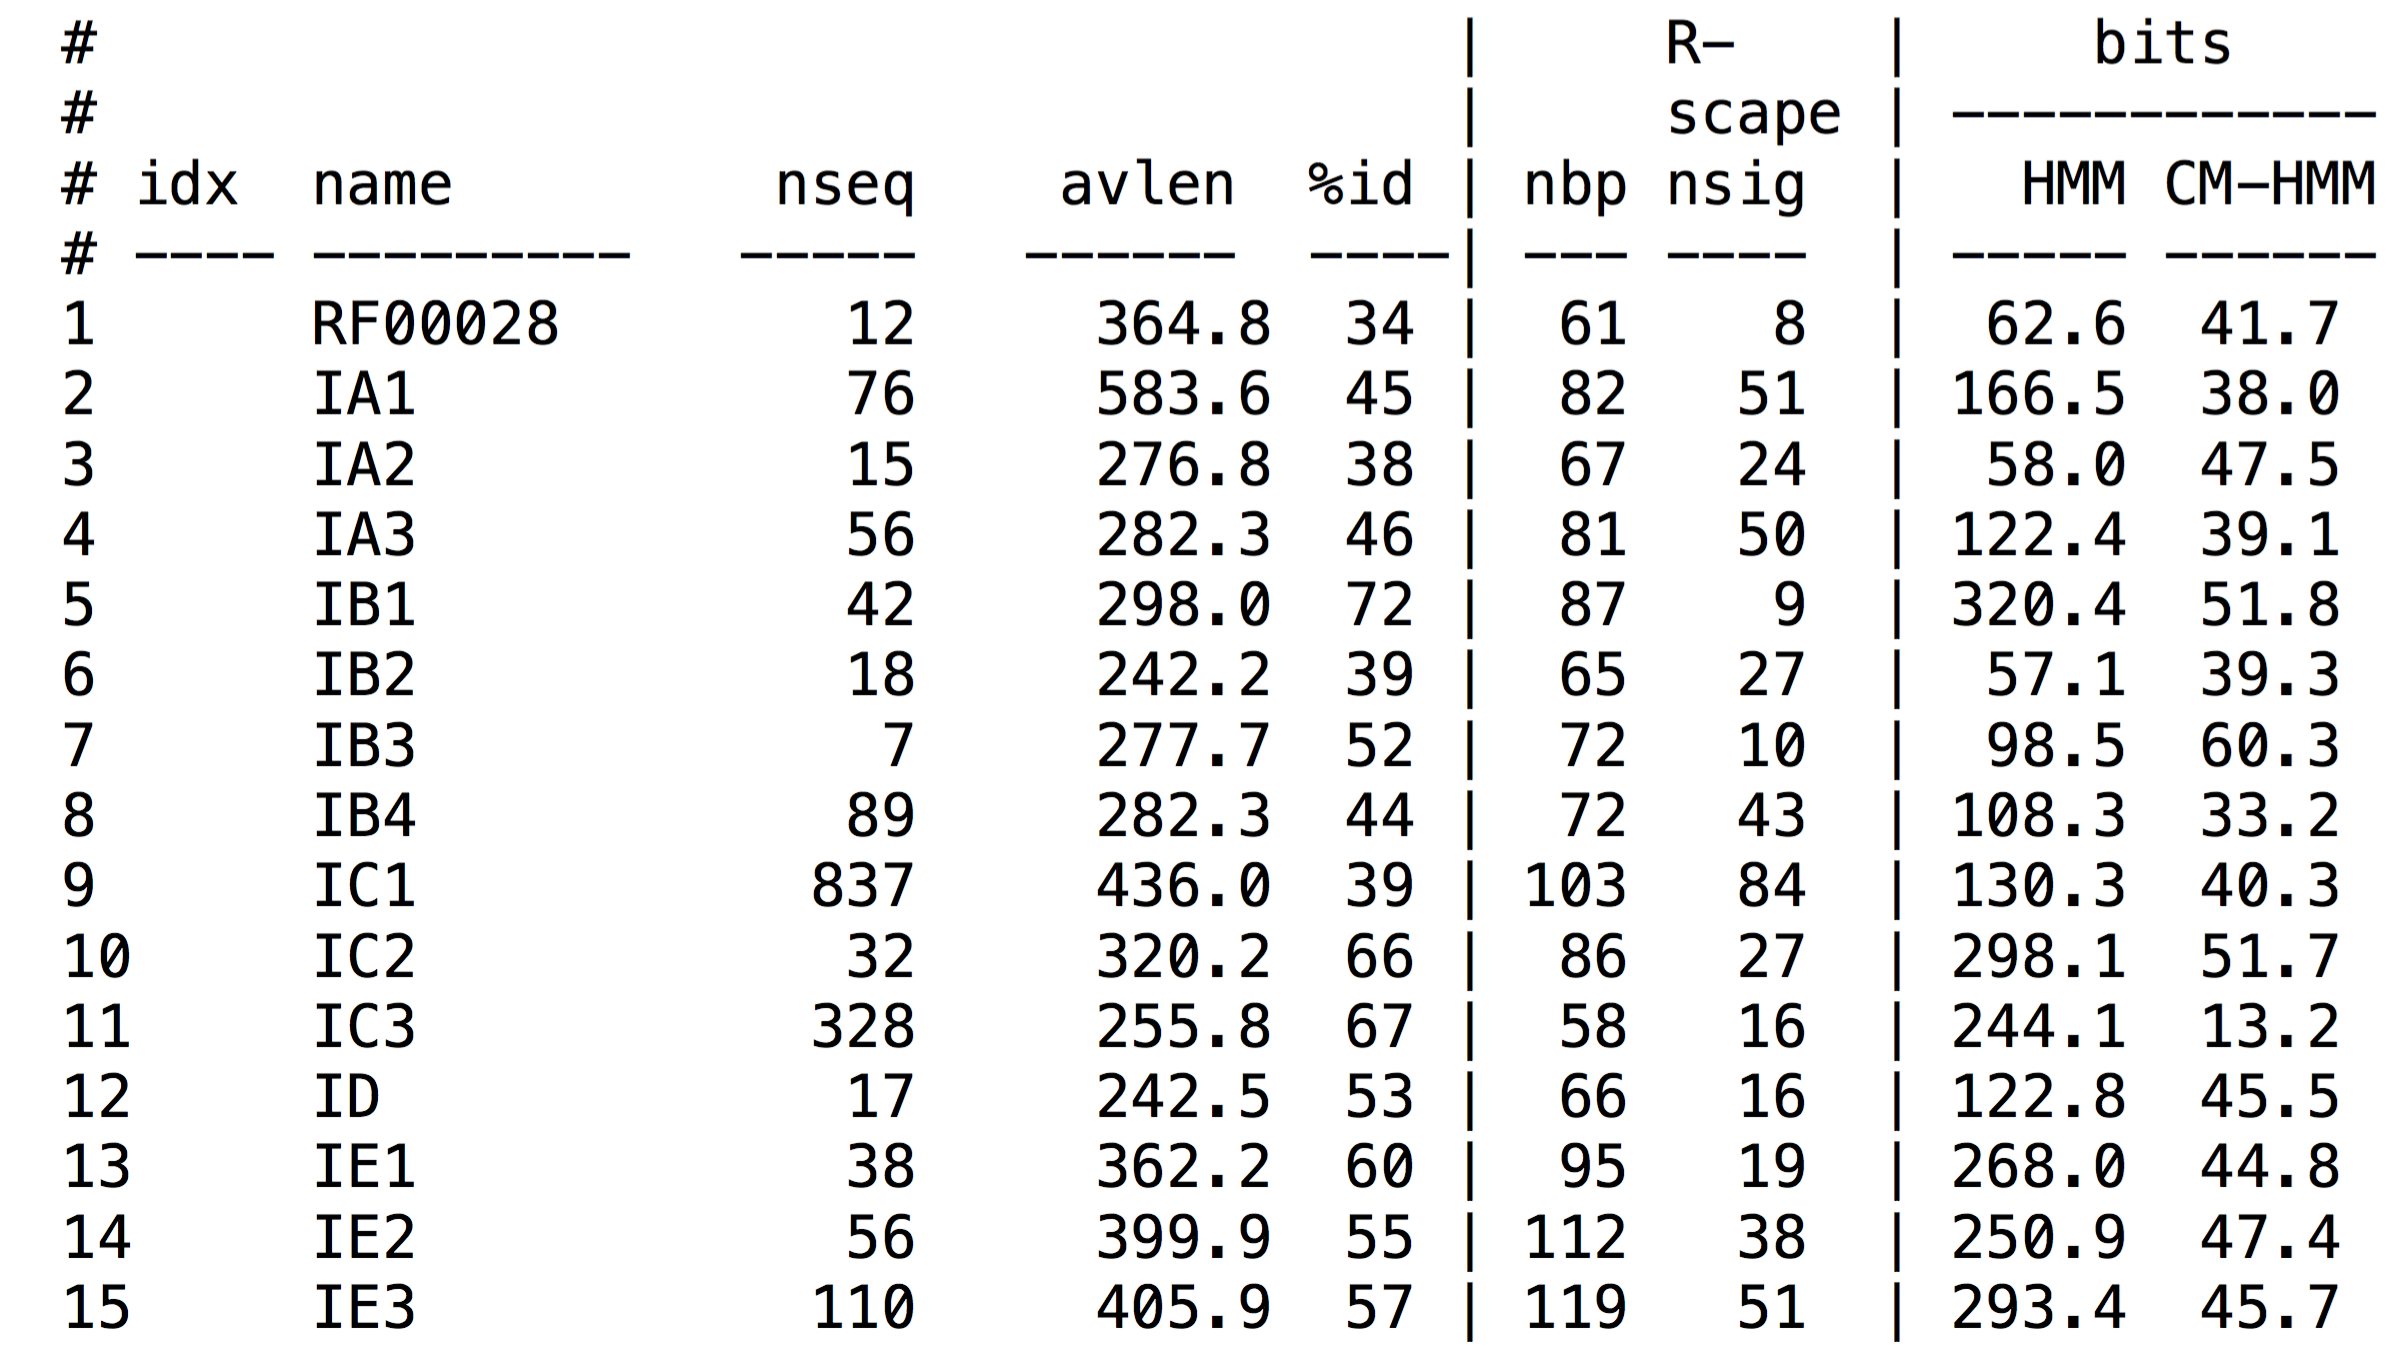
\includegraphics[width=8in]{figs/GISSD-stats-zoomed}}

\vfill
\end{slide}
%%%%%%%%%%%%%%%%%%%%%%%%%%%%%%%%%%%%%%%%%%%%%%%%%%%%%%%%%%%%%%%%%%%%%%%%%%
\begin{slide}
\begin{center}
\textbf{Searching Rfamseq with GISSD models}
\end{center}

%\small
%\begin{center}
%\begin{tabular}{l|r|rrr|r}
%\tt
%        & \# RF00028 & \# hits   & \# hits& \# hits& total     \\
%type    & seed seqs  & total     & common & unique & CPU hours \\ \hline
%IA1     & 3          &  814      & 385    & 425    & 1076 \\
%IA2     & 1          &  1722     & 823    & 899    & 50 \\
%IA3     &            &   958     & 401    & 557    & 14 \\
%IB1     &            &  3949     & 1033   & 2916   & 32 \\
%IB2     &            & 1861     & 467    & 1394   & 31 \\
%IB3     &            & 479     & 136    & 343    & 40 \\
%IB4     &  1         & 5717     & 2400   & 3317   & 39 \\
%IC1     &  3         & 8475     & 5385   & 3090   & 24 \\
%IC2     &            & 4870     & 3858   & 1012   & 22 \\
%IC3     & 4          & 72692     & 66033  & 6659   & 136 \\
%ID      &            & 572     & 0      & 572    & 29 \\
%IE1     &            & 1305     & 10     & 1295   & 12 \\
%IE2     &            & 1377     & 8      & 1369   & 12 \\
%IE3     &            & 1379     & 1      & 1378   & 13 \\
%        &            &          &        &        &    \\
%total   & 12         & 106170*   & 80940* & 25226  & 1530 \\
%        &           &           &        &    \\
%RF00028 & -         & 71421     & 71421  & -      & 125 \\
%\end{tabular}

\tt
\small
\begin{center}
\begin{tabular}{l|r|rrr}
        & \# RF00028 & \# hits   & \# hits& \# hits\\
type    & seed seqs  & total     & common & unique \\ \hline
IA1     & 3          &  814      & 385    & 425    \\
IA2     & 1          &  1722     & 823    & 899    \\
IA3     &            &   958     & 401    & 557    \\
IB1     &            &  3949     & 1033   & 2916   \\
IB2     &            & 1861     & 467    & 1394   \\
IB3     &            & 479     & 136    & 343    \\
IB4     &  1         & 5717     & 2400   & 3317   \\
IC1     &  3         & 8475     & 5385   & 3090   \\
IC2     &            & 4870     & 3858   & 1012   \\
IC3     & 4          & 72692     & 66033  & 6659   \\
ID      &            & 572     & 0      & 572    \\
IE1     &            & 1305     & 10     & 1295   \\
IE2     &            & 1377     & 8      & 1369   \\
IE3     &            & 1379     & 1      & 1378   \\
        &            &          &        &        \\
%total   & 12         & 106170*   & 80940* & 25226*  \\
total   & 12         & 106170*   & 80940* &  16842 \\
        &           &           &        \\
RF00028 & -         & 71421     & 71421  & -      \\
\end{tabular}

\begin{description}
\item[*] contains overlaps
\end{description}


\end{center}

\vfill
\end{slide}
%%%%%%%%%%%%%%%%%%%%%%%%%%%%%%%%%%%%%%%%%%%%%%%%%%%%%%%%%%%%%%%%%%%%%%%%%
\begin{slide}
\center{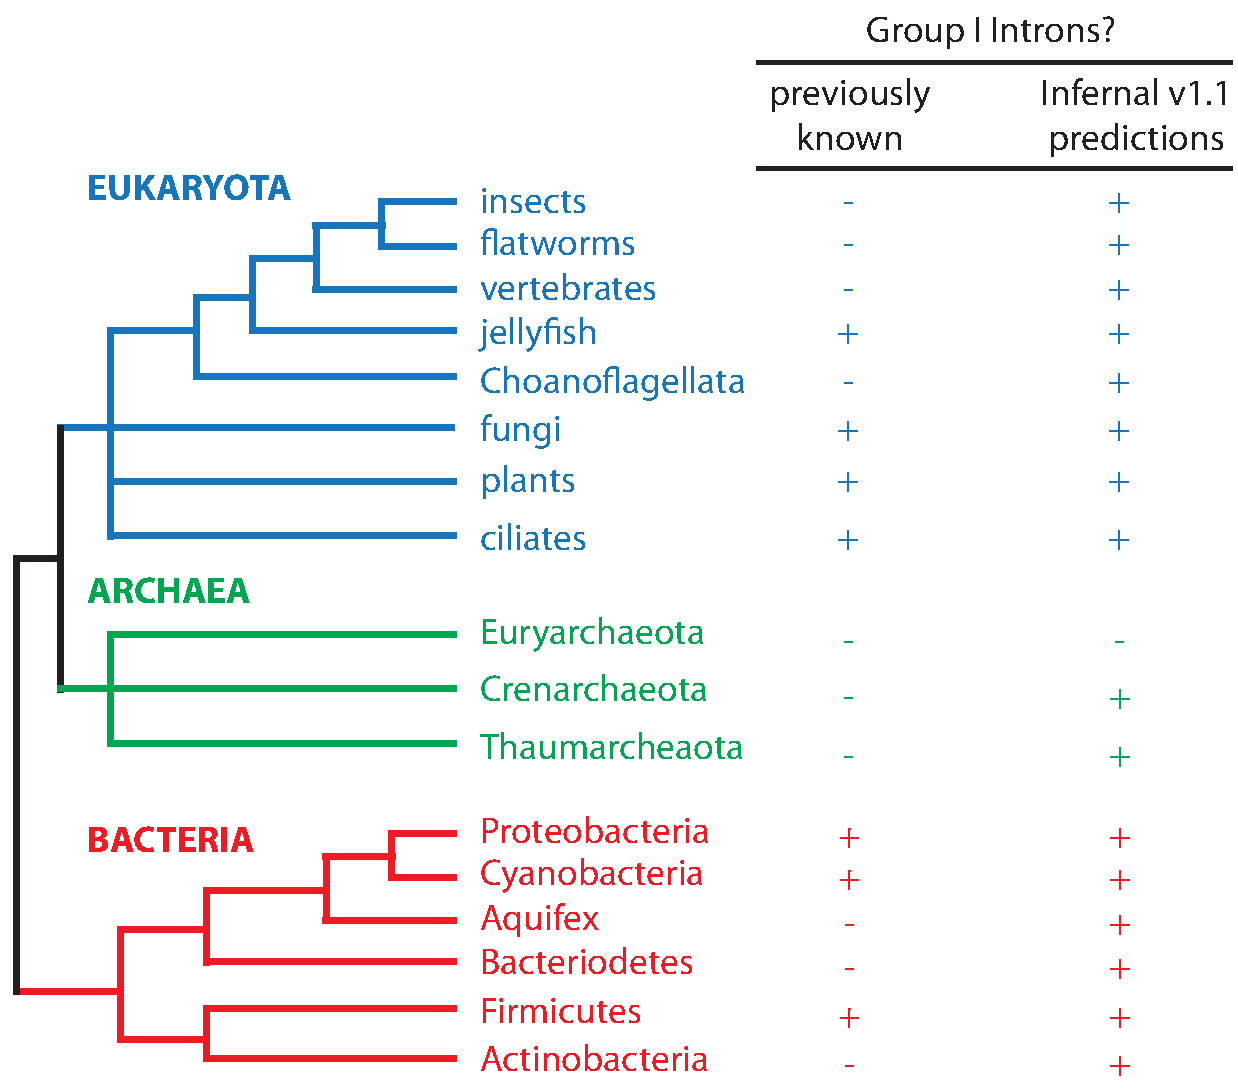
\includegraphics[height=8in]{figs/sean-slide-012215-gp1i-distro}}
\vfill
\end{slide}
%%%%%%%%%%%%%%%%%%%%%%%%%%%%%%%%%%%%%%%%%%%%%%%%%%%%%%%%%%%%%%%%%%%%%%%%%
\begin{slide}
\begin{center}
\textbf{Homology searches for group I introns in Archaea}
\end{center}
%
\small
\begin{itemize}
\item downloaded all archaeal sequences in GenBank (6.7Gb as of Sept
  2017)
\item searched archaeal sequences with all GISSD models + RF00028 with
  default cmsearch parameters and with \texttt{--anytrunc}
\item 95 non-overlapping hits with $E < 0.01$
  corresponding\footnote{as determined via manual sequence analysis by Tom Jones} to 39
  group I intron candidates (12 IA3 and 27 IB4)
\item 30/39 introns have at least one hit with $E < 10^{-10}$ 
\item 36 within LSU rRNA, 3 within SSU rRNA
\item All IA3s are in one of two LSU insertion positions:
  \begin{itemize}
  \item LSU/2593 (N=10)
  \item LSU/2500 (N=2)
  \end{itemize}
\item All IB4s are in one of two LSU insertion positions and one SSU
  position:
  \begin{itemize}
  \item LSU/1931 (N=15)
  \item LSU/1923 (N=9)
  \item SSU/1498 (N=3)
  \end{itemize}  
\end{itemize}  

\vfill
\end{slide}
%%%%%%%%%%%%%%%%%%%%%%%%%%%%%%%%%%%%%%%%%%%%%%%%%%%%%%%%%%%%%%%%%%%%%%%%%%
\begin{slide}

\center{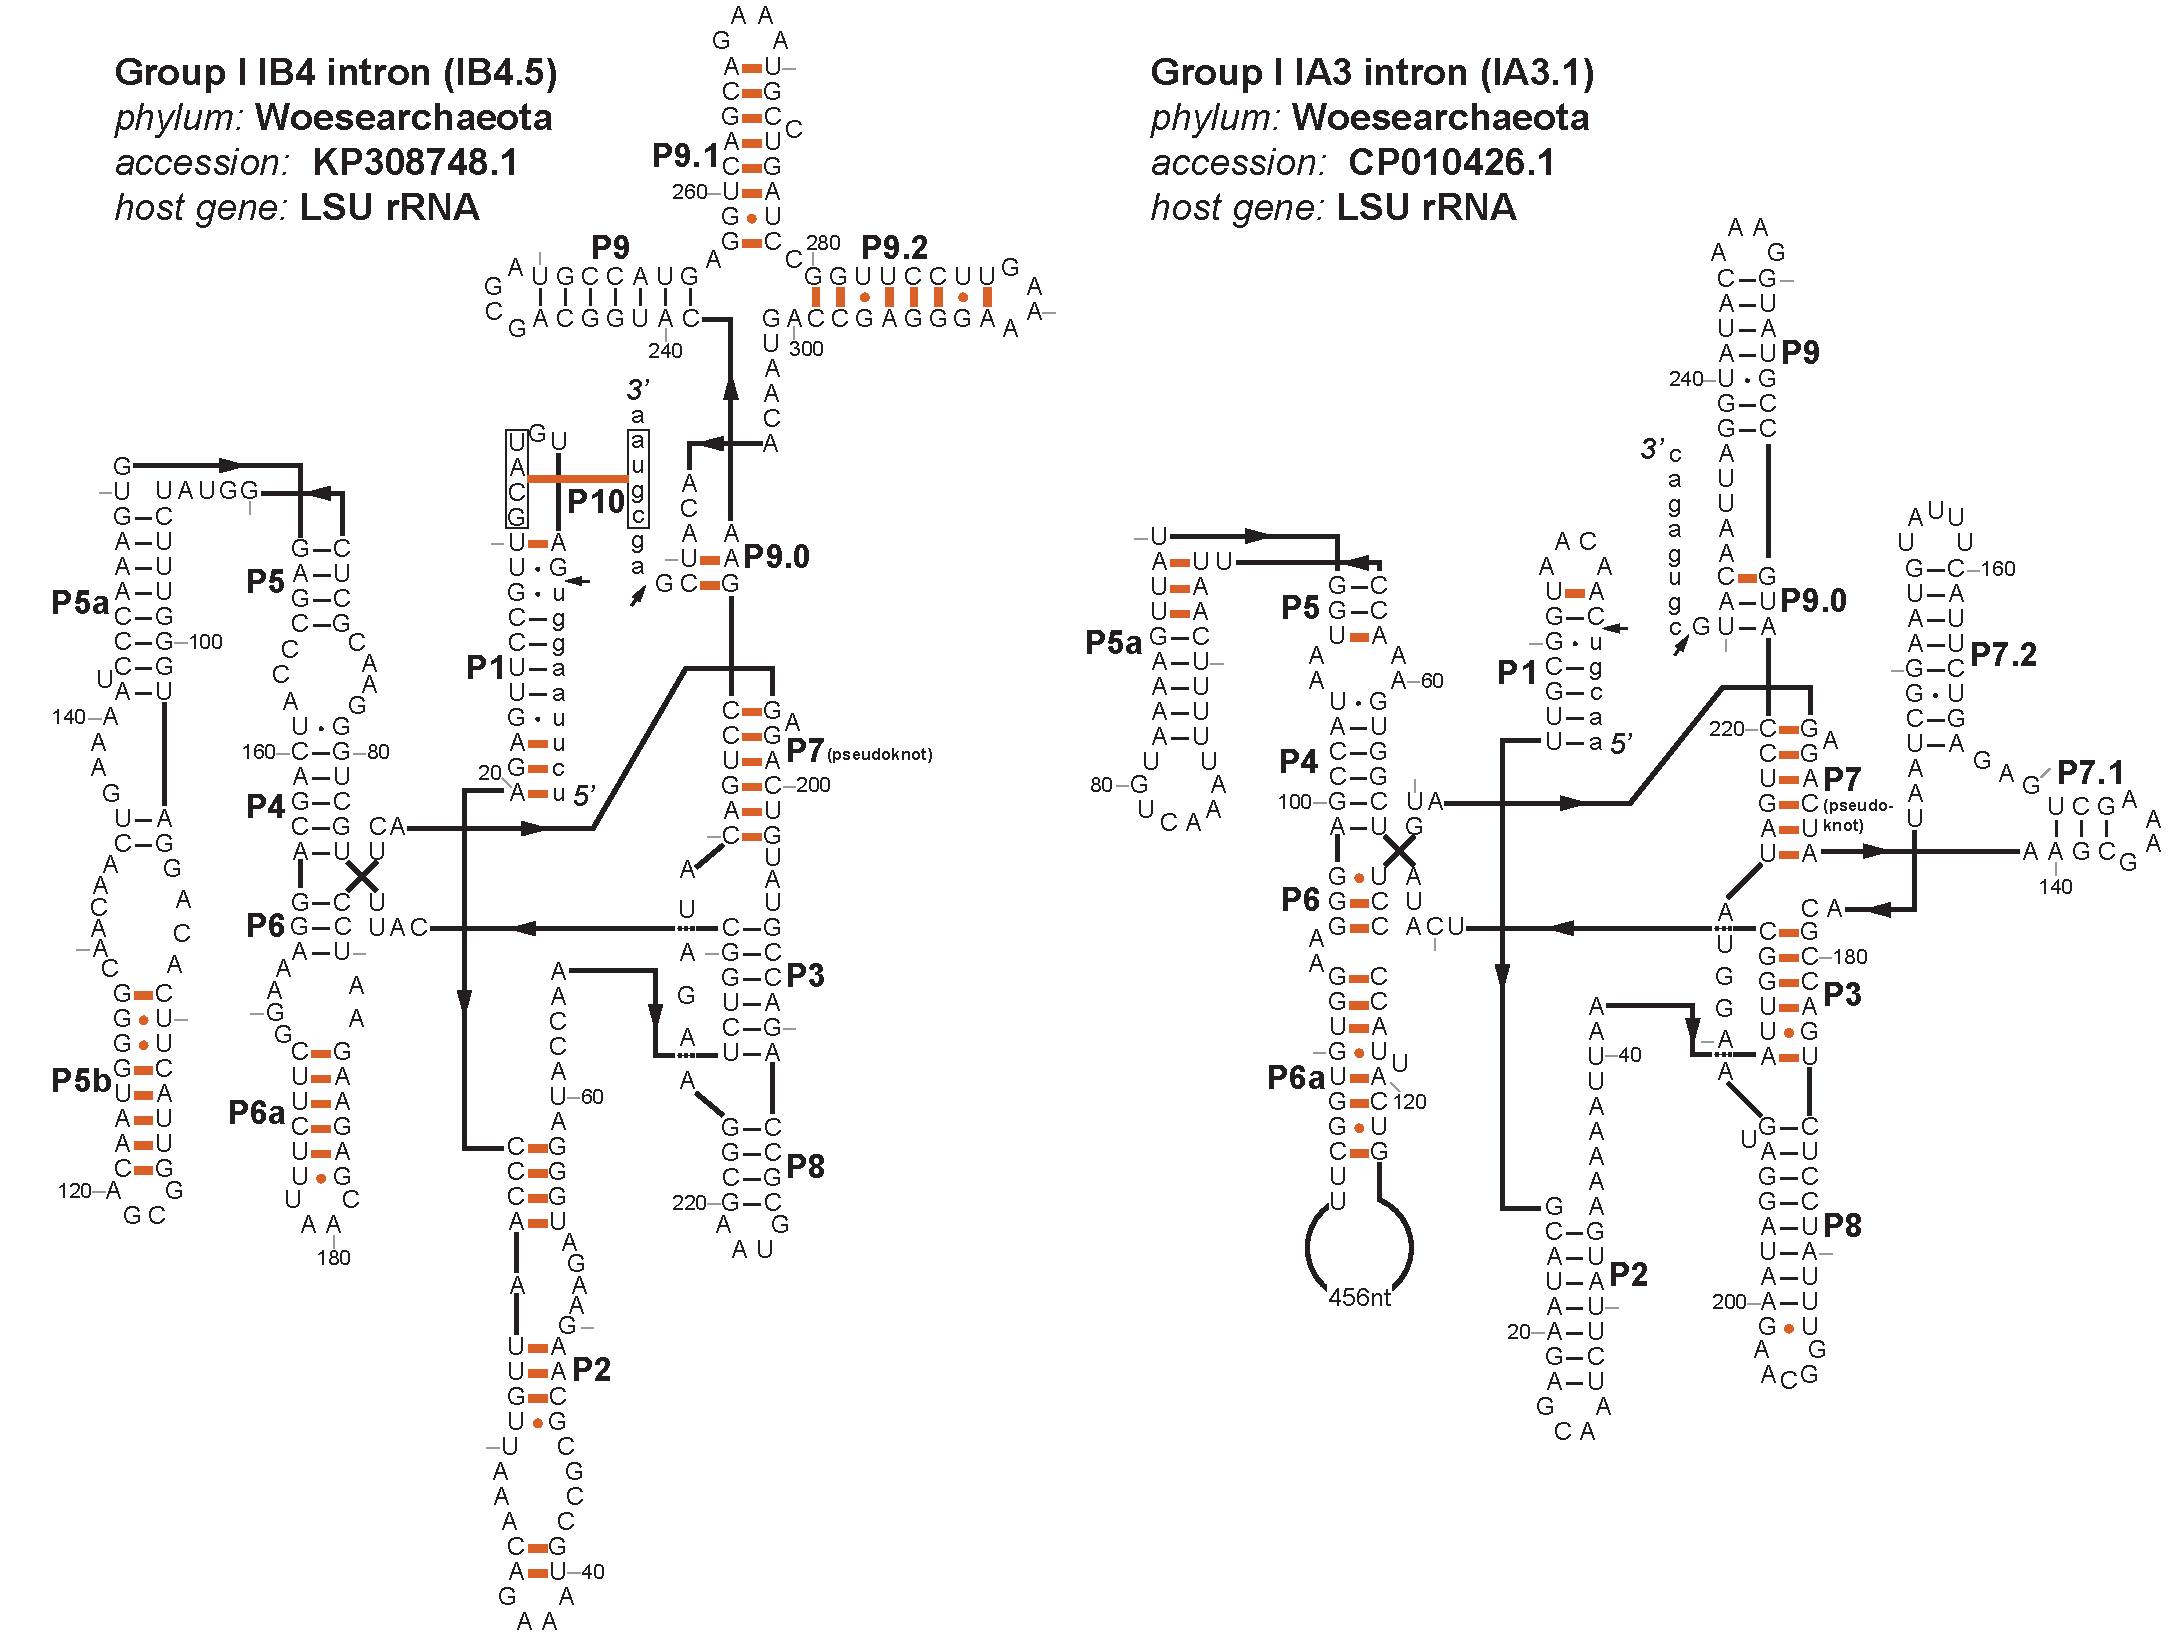
\includegraphics[width=10in]{figs/gp1-fig2-ss}}\footnote{
E. P. Nawrocki, T. A. Jones, and S. R. Eddy, NAR, 2018, gky414}

\vfill
\end{slide}
%%%%%%%%%%%%%%%%%%%%%%%%%%%%%%%%%%%%%%%%%%%%%%%%%%%%%%%%%%%%%%%%%%%%%%%%%
\begin{slide}
\begin{center}
\textbf{Could archaeal group I introns have evolved into BHB introns?}
\end{center}
\center{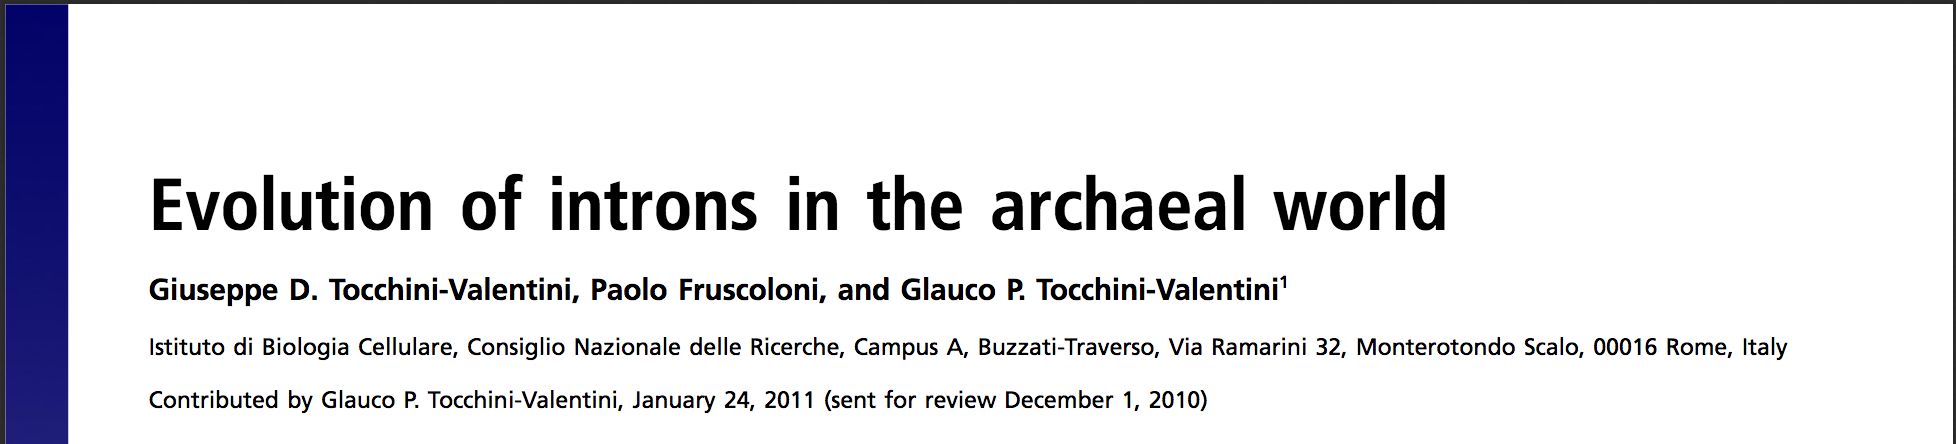
\includegraphics[width=8in]{figs/Tocchini-Valentini-title-screenshot}}\footnote{PNAS March 22, 2011. 108 (12) 4782-4787;}

\textbf{Archaeal group I introns can occur in same host gene as BHB introns}

\center{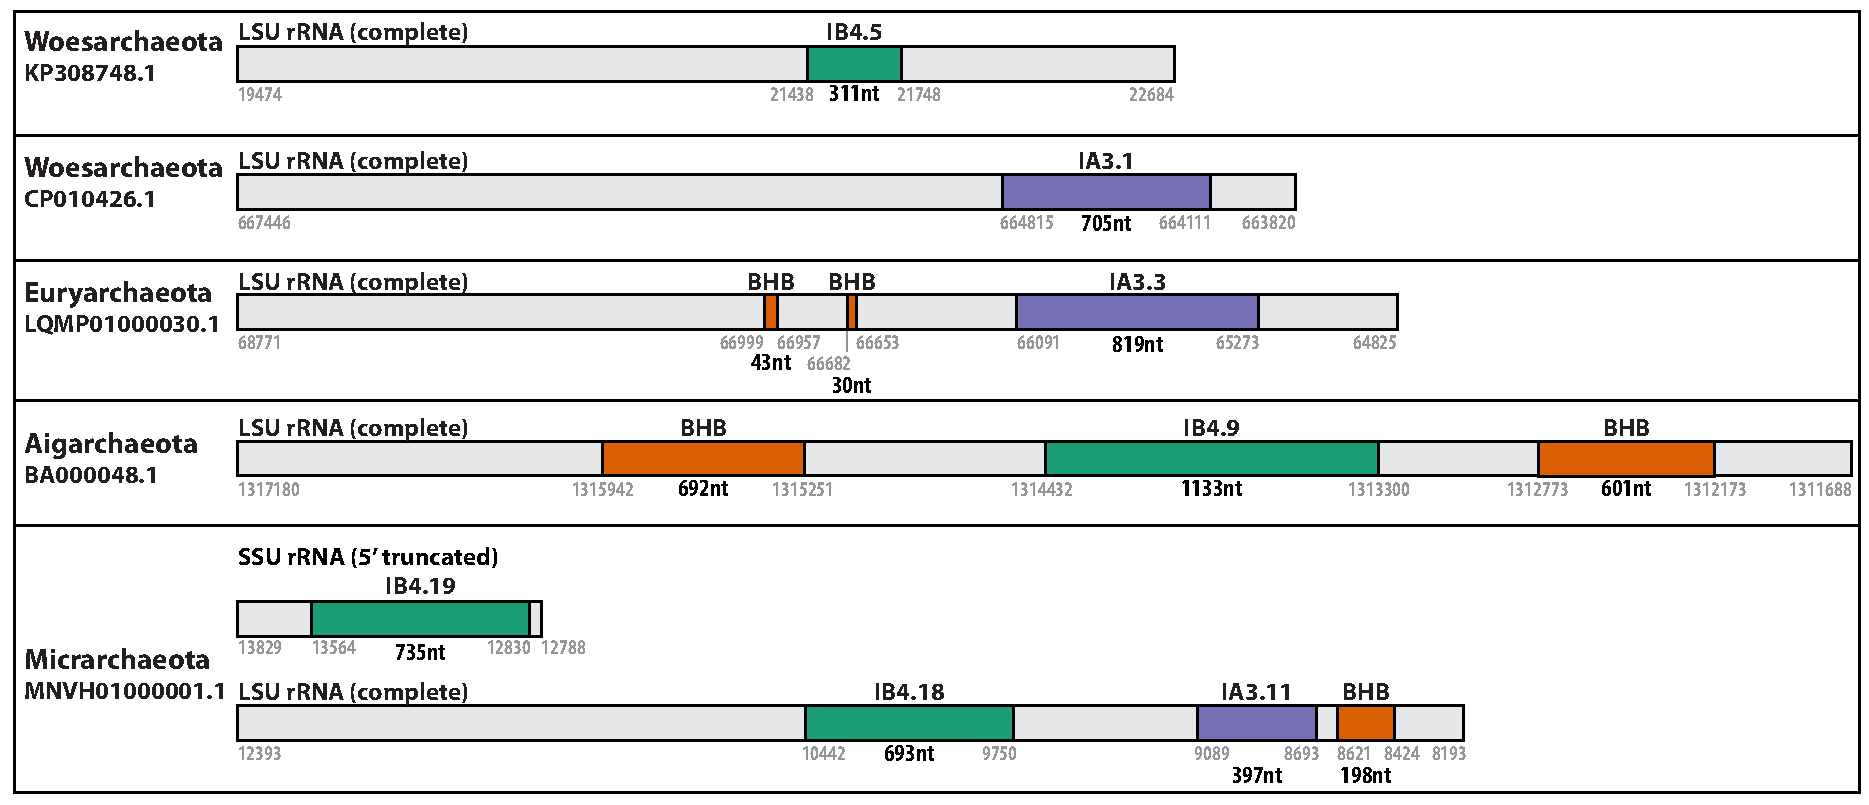
\includegraphics[width=10in]{figs/gp1-fig1-schematic}}
\vfill
\end{slide}
%%%%%%%%%%%%%%%%%%%%%%%%%%%%%%%%%%%%%%%%%%%%%%%%%%%%%%%%%%%%%%%%%%%%%%%%%
\begin{slide}
\begin{center}
\textbf{Group I introns are widespread in Archaea}
\end{center}

\center{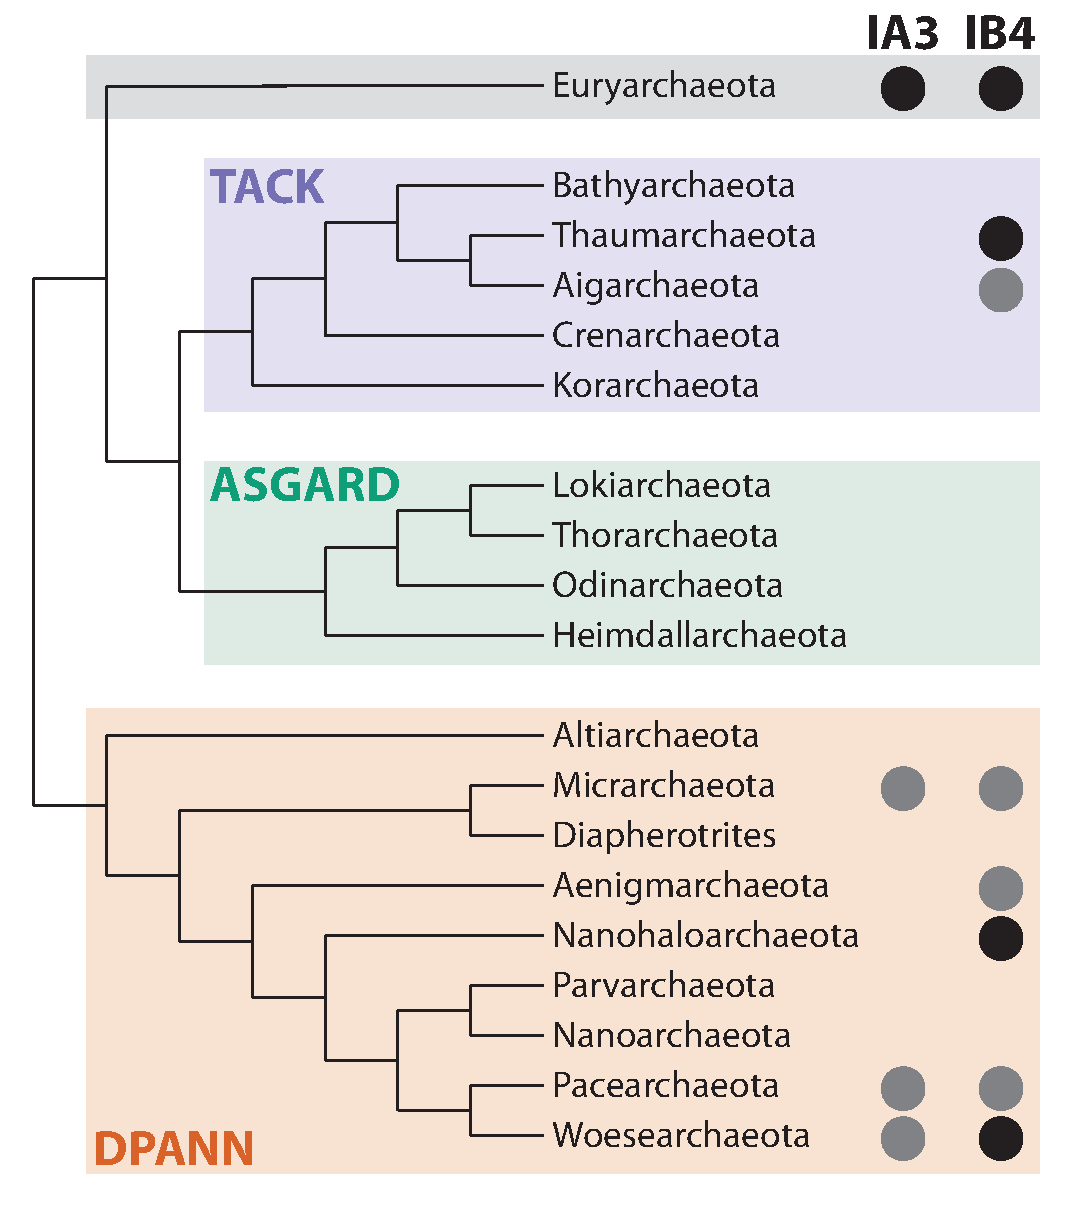
\includegraphics[height=6.5in]{figs/gp1-fig3-cladogram}}

\vfill
\end{slide}
%%%%%%%%%%%%%%%%%%%%%%%%%%%%%%%%%%%%%%%%%%%%%%%%%%%%%%%%%%%%%%%%%%%%%%%%%
\begin{slide}

\large
\begin{center}
\large{\textbf{Acknowledgements}} \\

\normalsize
\vspace{0.5in}

\begin{tabular}{l|l}
\textbf{Harvard/Janelia} & \textbf{NCBI} \\
Sean Eddy                &  Alejandro Sch\"{a}ffer \\
Tom Jones                &  David Landsman \\
Diana Kolbe              &  Jim Ostell \\
Travis Wheeler           &  David Lipman \\
Elena Rivas              &  \\
Michael Farrar           & \\
                & \\ \hline
                & \\
\textbf{GISSD}  & \textbf{David Haussler's group} \\
Yu Zhou         & Yasu Sakakibara \\
Chen Lu         &  (CM-like models in 1994) \\
Qi-Jia Wu       &  \\
Yu Wang         &  \\
Zhi-Tao Sun     &  \\
Jia-Cong Deng   &  \\
Yi Zhang        &  \\
\end{tabular}

\end{center}

\vfill
\end{slide}
%%%%%%%%%%%%%%%%%%%%%%%%%%%%%%%%%%%%%%%%%%%%%%%%%%%%%%%%%%%%%%%%%%%%%%
%%%%%%%%%%%%%%%%%%%%%%%%%%%%%%%%%%%%%%%%%%%%%%%%%%%%%%%%%%%%%%%%%%%%%%
\end{document}


\begin{slide}

\large
\begin{center}
\large{\textbf{Acknowledgements}} \\

\normalsize
\vspace{0.5in}

\textbf{Harvard/Janelia} \\
Sean Eddy \\
Diana Kolbe \\
Travis Wheeler \\
Elena Rivas \\
Tom Jones \\
Michael Farrar \\

\vspace{0.5in}
\textbf{David Haussler's group (CM-like models in 1994)} \\
Yasu Sakakibara\\

\vspace{0.5in}

\textbf{NCBI} \\
Alejandro Sch\"{a}ffer \\
David Landsman \\
Jim Ostell \\
David Lipman \\

\end{center}

\vfill
\end{slide}
%%%%%%%%%%%%%%%%%%%%%%%%%%%%%%%%%%%%%%%%%%%%%%%%%%%%%%%%%%%%%%%%%%%%%%
\end{document}
%%%%%%%%%%%%%%%%%%%%%%%%%%%%%%%%%%%%%%%%%%%%%%%%%%%%%%%%%%%%%%%%%%%%%%
%%%%%%%%%%%%%%%%%%%%%%%%%%%%%%%%%%%%%%%%%%%%%%%%%%%%%%%%%%%%%%%%%%%%%%
%%%%%%%%%%%%%%%%%%%%%%%%%%%%%%%%%%%%%%%%%%%%%%%%%%%%%%%%%%%%%%%%%%%%%%
%%%%%%%%%%%%%%%%%%%%%%%%%%%%%%%%%%%%%%%%%%%%%%%%%%%%%%%%%%%%%%%%%%%%%%
\begin{slide}
\begin{center}

\textbf{Rfam used BLAST filters from 2003 to 2012}

\end{center}

\begin{itemize}
\item Rfam includes $>$ 2000 RNA families, each represented by an
  alignment, CM and set of predicted homologs in a large database (Rfamseq).
\end{itemize}

\center{\includegraphics[width=8in]{figs/rfam-search-1}}

\vfill
\end{slide}
%%%%%%%%%%%%%%%%%%%%%%%%%%%%%%%%%%%%%%%%%%%%%%%%%%%%%%%%%%%%%%%%%%%%%%
\begin{slide}
\begin{center}

\textbf{Rfam used BLAST filters from 2003 to 2012}

\end{center}

\begin{itemize}
\item Rfam includes $>$ 2000 RNA families, each represented by an
  alignment, CM and set of predicted homologs in a large database (Rfamseq).
\end{itemize}

\center{\includegraphics[width=8in]{figs/rfam-search-2}}

\vfill
\end{slide}
%%%%%%%%%%%%%%%%%%%%%%%%%%%%%%%%%%%%%%%%%%%%%%%%%%%%%%%%%%%%%%%%%%%%%%
\begin{slide}
\begin{center}

\textbf{Rfam 12.0 (2014)\footnote{Nawrocki, Burge et. al, NAR 43:D130-D137, 2015.}, 
first release without BLAST filtering}
\end{center}

\center{\includegraphics[width=8in]{figs/rfam-search-3}}

%\begin{center}
%\small
%Search results against Rfamseq for 200 random families:
%\begin{tabular}{l|rrr}
%strategy                   & time (h) & \# hits & \# unique hits \\ \hline
%Old (BLAST + Infernal 1.0) & 4069.8   &  179681 & 53 \\
%New (Infernal 1.1)         & 4222.2   &  201814 & 22312 \\
%\end{tabular}
%\end{center}

\vfill
\end{slide}
%%%%%%%%%%%%%%%%%%%%%%%%%%%%%%%%%%%%%%%%%%%%%%%%%%%%%%%%%%%%%%%%%%%%%%
\begin{slide}
\begin{center}

\textbf{Rfam 12.0 (2014)\footnote{Nawrocki, Burge et. al, NAR 43:D130-D137, 2015.}, 
first release without BLAST filtering}

\end{center}

\begin{center}
Search results against Rfamseq for 200 random families:

\medskip

\begin{tabular}{l|r|r|r}
strategy                   & time (h) & \# hits & \# unique hits \\ \hline
& & & \\
Old (BLAST + Infernal 1.0) & 4069.8   &  179,681 & 53 \\
& & & \\
New (Infernal 1.1)         & 4222.2   &  201,814 & 22,312 \\
\end{tabular}
\end{center}

\vfill
\end{slide}
%%%%%%%%%%%%%%%%%%%%%%%%%%%%%%%%%%%%%%%%%%%%%%%%%%%%%%%%%%%%%%%%%%%%%%
%\begin{slide}
%\begin{center}
%\small
%\end{center}
%
%\center{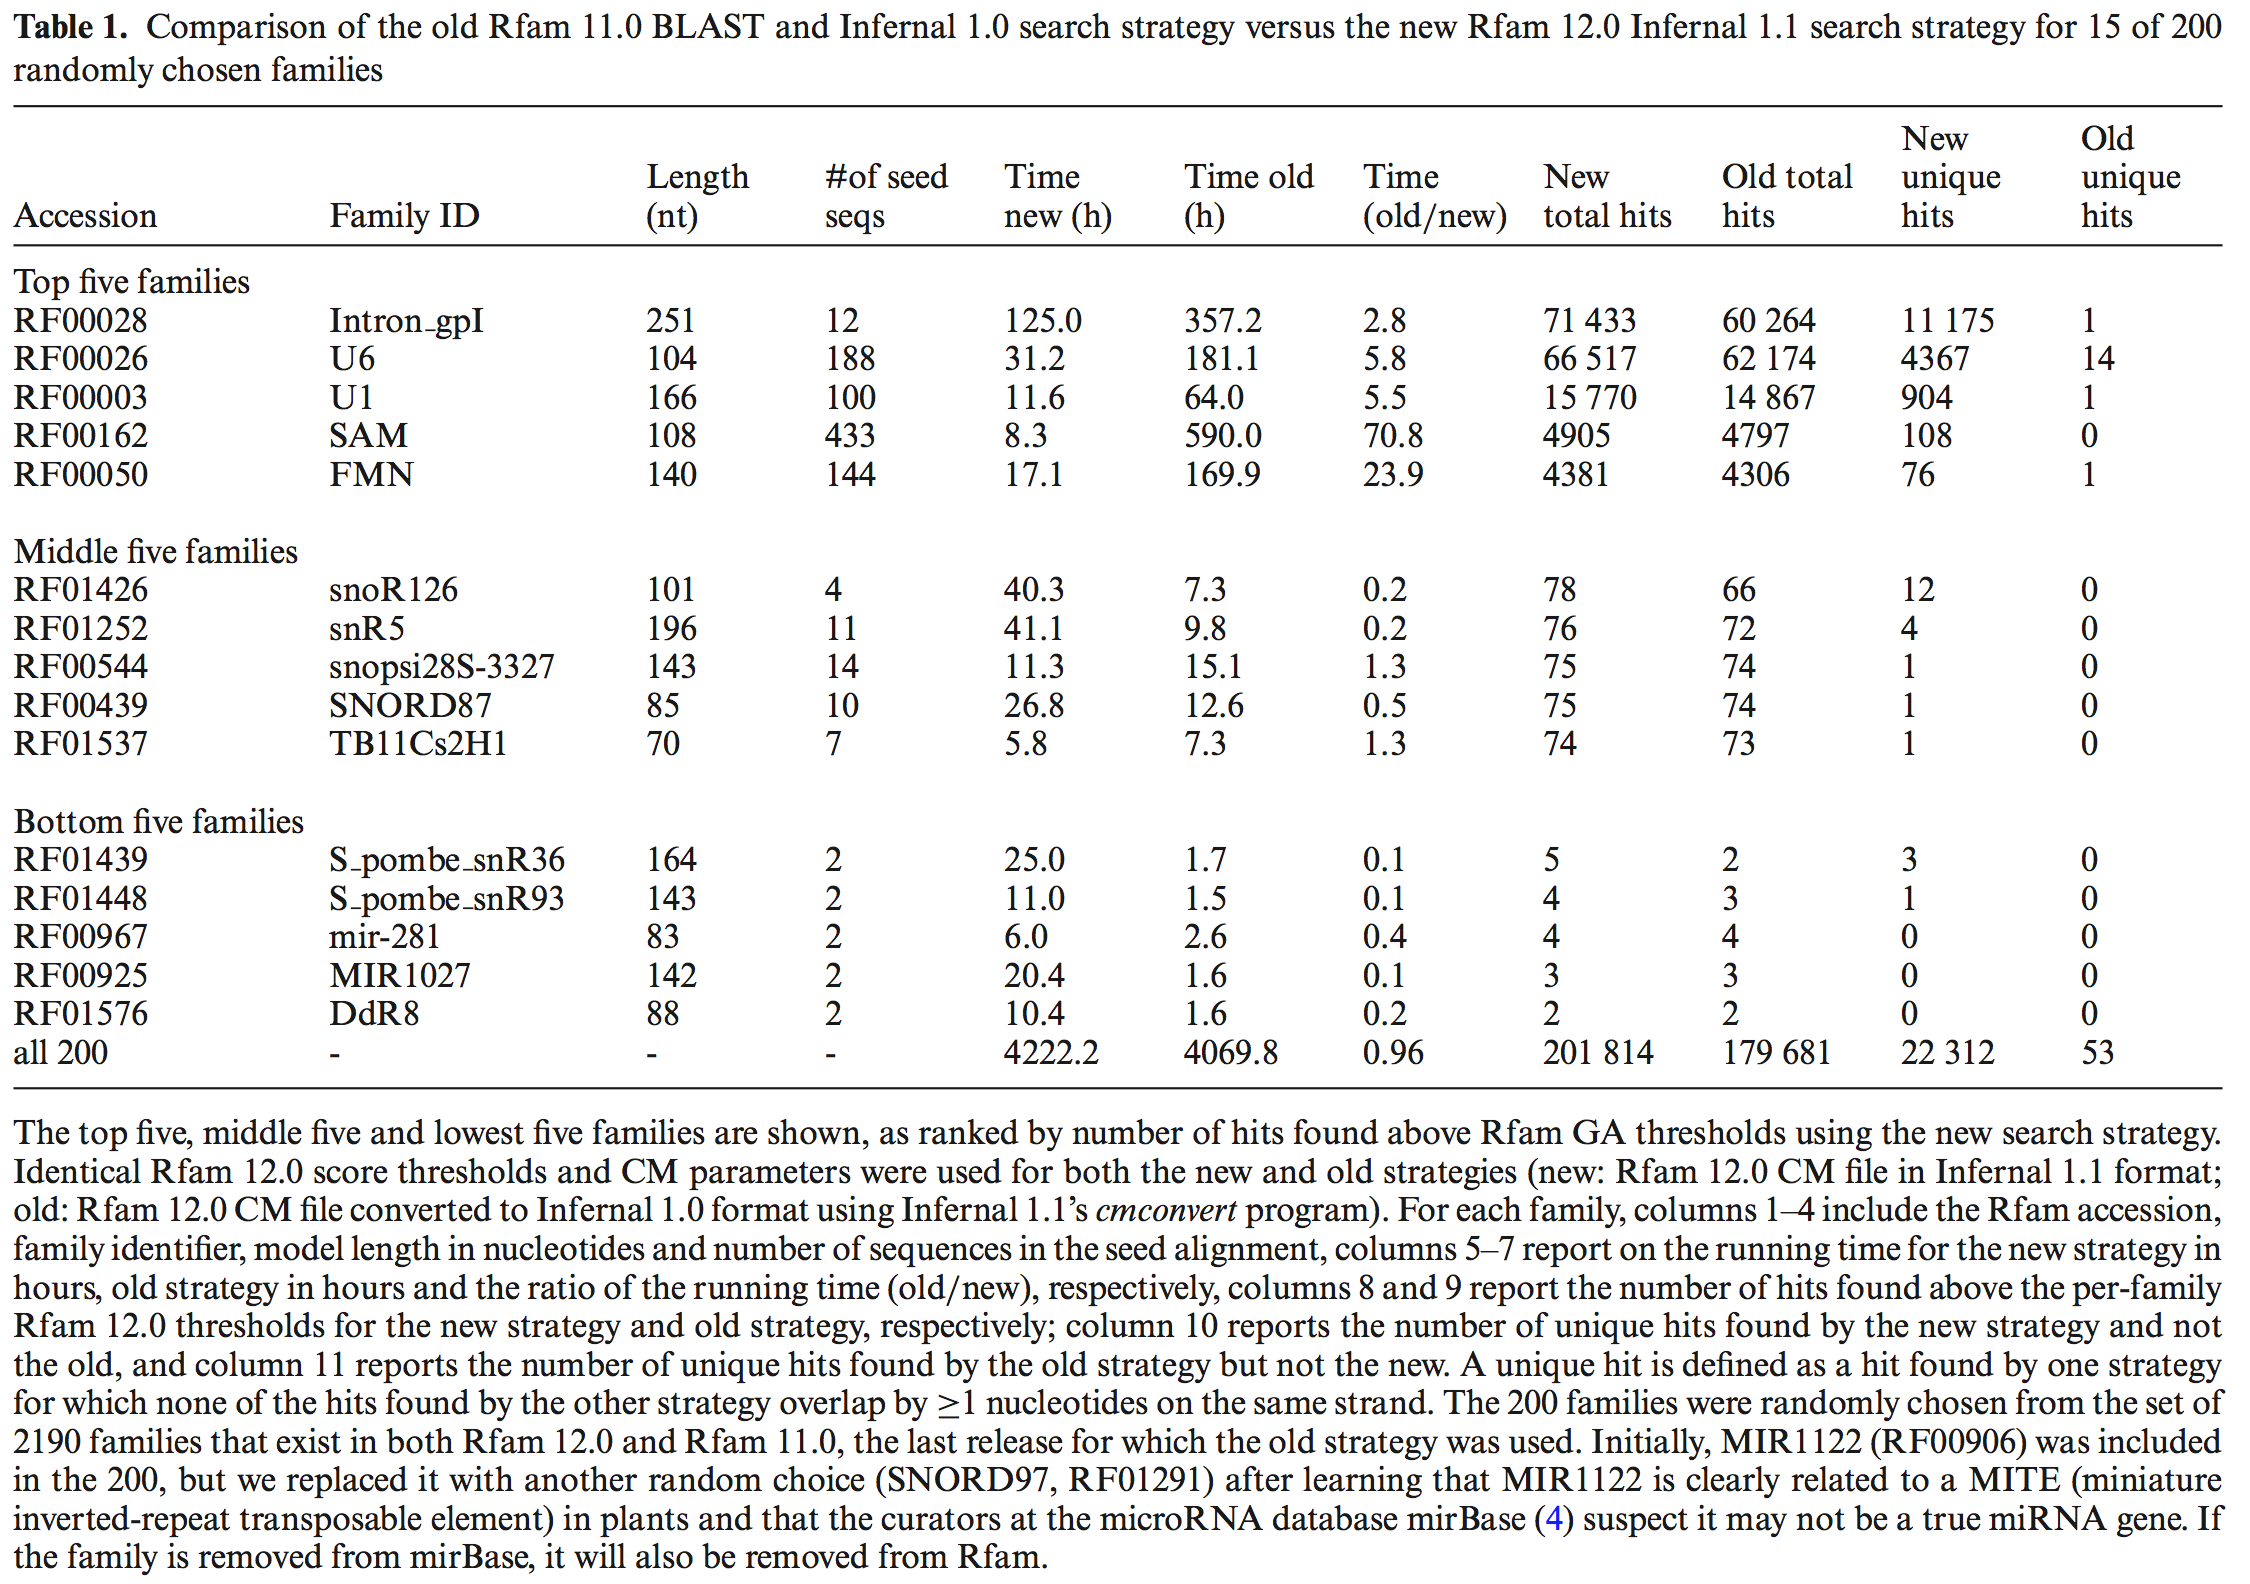
\includegraphics[width=10.5in]{figs/rfam-nar-table1-published}}
%
%\vfill
%\end{slide}
%%%%%%%%%%%%%%%%%%%%%%%%%%%%%%%%%%%%%%%%%%%%%%%%%%%%%%%%%%%%%%%%%%%%%%
\begin{slide}
\begin{center}
%\small
\textbf{It is now easier to use Rfam/Infernal to annotate your own datasets}
\end{center}

\center{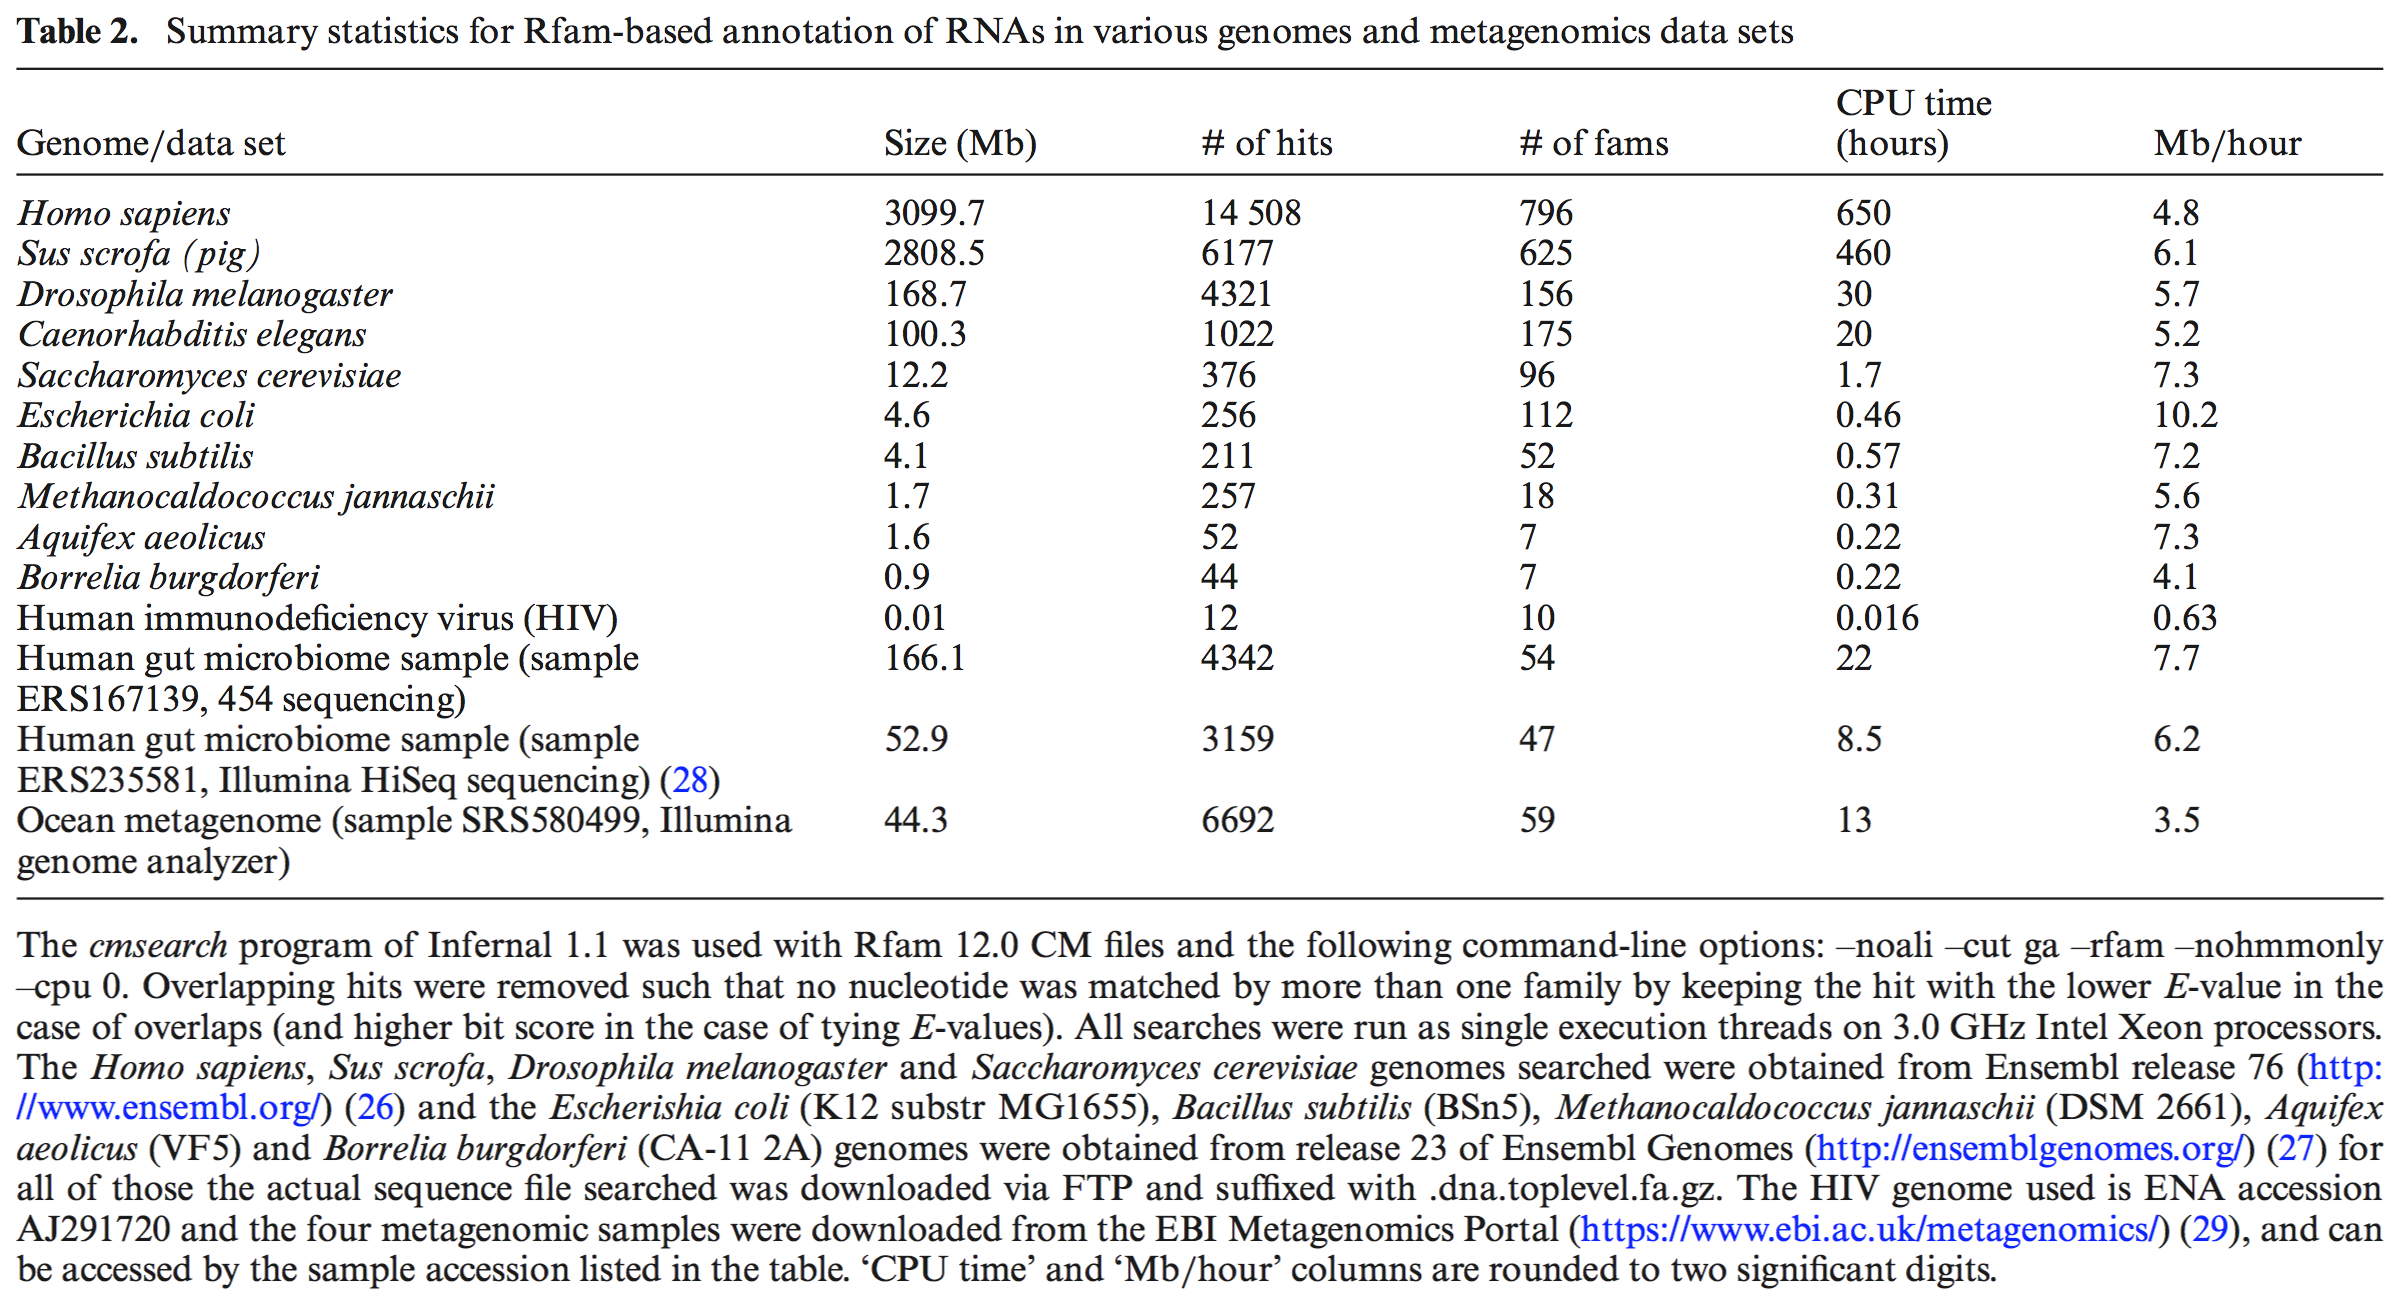
\includegraphics[width=10.5in]{figs/rfam-nar-table2-published}}

\vfill
\end{slide}
%%%%%%%%%%%%%%%%%%%%%%%%%%%%%%%%%%%%%%%%%%%%%%%%%%%%%%%%%%%%%%%%%%%%%%%%%%
\begin{slide}
\begin{center}
\textbf{Infernal 1.1 finds 11,000 new group I intron candidates}
\end{center}

%\center{\includegraphics[width=10.5in]{figs/rfam-nar-table1-published-gp1i-yellow}}
\center{\includegraphics[width=10.5in]{figs/rfam-nar-table1-published-gp1i-yellow-top5only}}

\vfill
\end{slide}
%%%%%%%%%%%%%%%%%%%%%%%%%%%%%%%%%%%%%%%%%%%%%%%%%%%%%%%%%%%%%%%%%%%%%%
\begin{slide}
\begin{center}
\textbf{Group I catalytic Introns}
\end{center}
%
\small
\begin{itemize}
\item self splicing ribozymes found in lower eukaryotes, higher
  plants, bacteria and bacteriophages
%\item core secondary structure (modeled by Rfam) consists of 9 paired
%  regions
\item often have ORFs (homing endonucleases) inserted in loop regions
\item genes they are found in:
\begin {itemize}
\item bacteria and mitochondria and chloroplast of lower euks: rRNA, mRNA, and tRNAs
\item higher plants mitochondria and chloroplast: a few tRNA and mRNA genes
\item nuclear lower eukaryotic genomes: only rRNA
%\item Gram positive bacteriophages: widely distributed
%\item Gram negative bacteriophages: T4, T-even and T7-like
\end{itemize}
\end{itemize}

%\center{\includegraphics[height=4in]{figs/gp1-schematic-small.png}}
\center{\includegraphics[height=4.5in]{figs/gp1-schematic-big.png}}


\vfill
\end{slide}
%%%%%%%%%%%%%%%%%%%%%%%%%%%%%%%%%%%%%%%%%%%%%%%%%%%%%%%%%%%%%%%%%%%%%%%%%%
\begin{slide}
\center{\includegraphics[height=8in]{figs/RF00028-ss-info-ss-1}}
\vfill
\end{slide}
%%%%%%%%%%%%%%%%%%%%%%%%%%%%%%%%%%%%%%%%%%%%%%%%%%%%%%%%%%%%%%%%%%%%%%%%%%
\begin{slide}
\center{\includegraphics[height=8in]{figs/RF00028-ss-mutinfo-ss-1}}
\vfill
\end{slide}
%%%%%%%%%%%%%%%%%%%%%%%%%%%%%%%%%%%%%%%%%%%%%%%%%%%%%%%%%%%%%%%%%%%%%%%%%%
\begin{slide}
\begin{center}
\small
\textbf{GISSD\footnote{Y. Zhou et. al, NAR, 2008. 36(suppl
    1), D31-D37.}: Group I Intron Sequence and Structure Database}
\end{center}

\center{\includegraphics[width=10in]{figs/gissd-banner}}

\center{\includegraphics[width=10in]{figs/gissd-alistat-ss-1}}

\vfill
\end{slide}
%%%%%%%%%%%%%%%%%%%%%%%%%%%%%%%%%%%%%%%%%%%%%%%%%%%%%%%%%%%%%%%%%%%%%%%%%%
\begin{slide}
\begin{center}
\textbf{Searching Rfamseq with GISSD models}
\end{center}

%\small
%\begin{center}
%\begin{tabular}{l|r|rrr|r}
%\tt
%        & \# RF00028 & \# hits   & \# hits& \# hits& total     \\
%type    & seed seqs  & total     & common & unique & CPU hours \\ \hline
%IA1     & 3          &  814      & 385    & 425    & 1076 \\
%IA2     & 1          &  1722     & 823    & 899    & 50 \\
%IA3     &            &   958     & 401    & 557    & 14 \\
%IB1     &            &  3949     & 1033   & 2916   & 32 \\
%IB2     &            & 1861     & 467    & 1394   & 31 \\
%IB3     &            & 479     & 136    & 343    & 40 \\
%IB4     &  1         & 5717     & 2400   & 3317   & 39 \\
%IC1     &  3         & 8475     & 5385   & 3090   & 24 \\
%IC2     &            & 4870     & 3858   & 1012   & 22 \\
%IC3     & 4          & 72692     & 66033  & 6659   & 136 \\
%ID      &            & 572     & 0      & 572    & 29 \\
%IE1     &            & 1305     & 10     & 1295   & 12 \\
%IE2     &            & 1377     & 8      & 1369   & 12 \\
%IE3     &            & 1379     & 1      & 1378   & 13 \\
%        &            &          &        &        &    \\
%total   & 12         & 106170*   & 80940* & 25226  & 1530 \\
%        &           &           &        &    \\
%RF00028 & -         & 71421     & 71421  & -      & 125 \\
%\end{tabular}


\small
\begin{center}
\begin{tabular}{l|r|rrr}
\tt
        & \# RF00028 & \# hits   & \# hits& \# hits\\
type    & seed seqs  & total     & common & unique \\ \hline
IA1     & 3          &  814      & 385    & 425    \\
IA2     & 1          &  1722     & 823    & 899    \\
IA3     &            &   958     & 401    & 557    \\
IB1     &            &  3949     & 1033   & 2916   \\
IB2     &            & 1861     & 467    & 1394   \\
IB3     &            & 479     & 136    & 343    \\
IB4     &  1         & 5717     & 2400   & 3317   \\
IC1     &  3         & 8475     & 5385   & 3090   \\
IC2     &            & 4870     & 3858   & 1012   \\
IC3     & 4          & 72692     & 66033  & 6659   \\
ID      &            & 572     & 0      & 572    \\
IE1     &            & 1305     & 10     & 1295   \\
IE2     &            & 1377     & 8      & 1369   \\
IE3     &            & 1379     & 1      & 1378   \\
        &            &          &        &        \\
%total   & 12         & 106170*   & 80940* & 25226*  \\
total   & 12         & 106170*   & 80940* &  16842 \\
        &           &           &        \\
RF00028 & -         & 71421     & 71421  & -      \\
\end{tabular}

\begin{description}
\item[*] contains overlaps
\end{description}


\end{center}

\vfill
\end{slide}
%%%%%%%%%%%%%%%%%%%%%%%%%%%%%%%%%%%%%%%%%%%%%%%%%%%%%%%%%%%%%%%%%%%%%%%%%
\begin{slide}
\center{\includegraphics[height=8in]{figs/sean-slide-012215-gp1i-distro}}
\vfill
\end{slide}
%%%%%%%%%%%%%%%%%%%%%%%%%%%%%%%%%%%%%%%%%%%%%%%%%%%%%%%%%%%%%%%%%%%%%%%%%
\begin{slide}
\begin{center}
\textbf{Annotation of thaumarchaeota candidate}
\end{center}

\center{\includegraphics[width=10in]{figs/anon-arc-2-gene-diagram}}

\vfill
\end{slide}
%%%%%%%%%%%%%%%%%%%%%%%%%%%%%%%%%%%%%%%%%%%%%%%%%%%%%%%%%%%%%%%%%%%%%%%%%
\begin{slide}
\begin{center}
\textbf{Thaumarchaeota group I structure}
\end{center}

\center{\includegraphics[height=6.5in]{figs/thaumarchaea-AP011865-1-classic-coke}}

\vfill
\end{slide}
%%%%%%%%%%%%%%%%%%%%%%%%%%%%%%%%%%%%%%%%%%%%%%%%%%%%%%%%%%%%%%%%%%%%%%%%%
\begin{slide}

\large
\begin{center}
\large{\textbf{Acknowledgements}} \\

\vspace{0.5in}

\normalsize
%\begin{tabular}{llllll}
%Sean Eddy           & & & & & Michael Brent \\ 
%Elena Rivas         & & & & & Jeremy Buhler \\
%Tom Jones           & & & & & Justin Fay \\
%Diana Kolbe         & & & & & Jeff Gordon \\
%Seolkyoung Jung     & & & & & Rob Mitra \\
%Sergi Castellano    & & & & & Gary Stormo \\
%Fred Davis          & & & & & \\
%Lee Henry           & & & & & \\
%Michael Farrar      & & & & & \\
%Travis Wheeler      & & & & & \\
\begin{tabular}{l|l}
\textbf{Janelia} & \textbf{EBI (Rfam)} \\ \hline
{\bf Sean Eddy}     & {\bf Alex Bateman} \\
Elena Rivas         & {\bf Rob Finn} \\
Travis Wheeler      & {\bf Sarah Burge} \\ 
{\bf Tom Jones}     & {\bf Evan Floden} \\
Diana Kolbe         & John Tate \\
Seolkyoung Jung     & Jen Daub \\
Rob Finn            & \\
Jody Clements       & \\
Fred Davis          & \\
Lee Henry           & \\
Michael Farrar      & \\
\end{tabular}

%\includegraphics[height=3in]{figs/jfrc-banner1}

\end{center}

\vfill
\end{slide}
%%%%%%%%%%%%%%%%%%%%%%%%%%%%%%%%%%%%%%%%%%%%%%%%%%%%%%%%%%%%%%%%%%%%%%
%%%%%%%%%%%%%%%%%%%%%%%%%%%%%%%%%%%%%%%%%%%%%%%%%%%%%%%%%%%%%%%
\begin{slide}
\begin{center}
\textbf{Is the added complexity worth it? \\
  RMARK: a challenging \underline{internal} RNA homology search
  benchmark}

\includegraphics[width=10in]{figs/rmark-tree-1}
\end{center}

\vfill
\end{slide}
%%%%%%%%%%%%%%%%%%%%%%%%%%%%%%%%%%%%%%%%%%%%%%%%%%%%%%%%%%%%%%%%%%%%%%
\begin{slide}
\begin{center}
\textbf{Is the added complexity worth it? \\
  RMARK: a challenging \underline{internal} RNA homology search
  benchmark}

\includegraphics[width=10in]{figs/rmark-tree-2}
\end{center}

\vfill
\end{slide}
%%%%%%%%%%%%%%%%%%%%%%%%%%%%%%%%%%%%%%%%%%%%%%%%%%%%%%%%%%%%%%%%%%%%%%
\end{document}
